\documentclass[a4paper,12pt]{article}
\usepackage[utf8]{inputenc}
\usepackage{polyglossia}
\setmainlanguage{spanish}
\usepackage{pythonhighlight}
\usepackage{multirow}
\usepackage{booktabs}
\usepackage{enumitem}
\usepackage{breakcites}
\usepackage{amsmath}
\usepackage{amsfonts}
\usepackage{tabularx}
\usepackage{pdfpages} 
\usepackage{changepage}
\usepackage{graphicx}
\usepackage{amsmath}
\usepackage{svg}
\usepackage[bookmarks = true, colorlinks=true, linkcolor = black, citecolor = black, menucolor = black, urlcolor = black]{hyperref}
\usepackage{lmodern}
\usepackage{listings}
\usepackage{adjustbox}
\usepackage{float}
\renewcommand{\baselinestretch}{1} % Interlineado. 1 es estandar
\usepackage[T1]{fontenc}
\usepackage[square,sort,comma,numbers]{natbib}
\usepackage{mathtools}
\usepackage{fancyhdr}
\fancyhead[R]{2021}\fancyhead[L]{UNC - FCEFyN} \fancyfoot[C]{\thepage}
\pagestyle{fancy}
\usepackage[numbered]{bookmark} % Para que figure las secciones en el PDF
\graphicspath{ {img/} }
\usepackage[normalem]{ulem}
\useunder{\uline}{\ul}{}
\DeclareMathOperator*{\argmax}{arg\,max}
\DeclareMathOperator*{\argmin}{arg\,min}
\author{Gerardo A. COLLANTE \\ Matrícula: 39.022.782 \\ Email: \href{mailto:gerardo.collante@unc.edu.ar}{gerardo.collante@unc.edu.ar} \\ Cel: 54 (03574) 650490}

\begin{document}

\makeatletter
\begin{titlepage}
				
	{\scshape\LARGE Universidad Nacional de Córdoba \par}
	%\vspace{1cm}
	{\Large Facultad de Ciencias Exactas, Físicas y Naturales \par}
	\vspace{0.5cm}
	\centering
	
\includegraphics[width=0.5\textwidth]{unc.png}
	\par\vspace{0.5cm}
	\vspace{0.5cm}
	{\scshape\Large Proyecto Final Integrador\par}
	\vspace{1cm}
	{\large\bfseries ``Predicción de cantidad de defectos graves en vehículos utilitarios en planta automotriz'' \par}
	
	\vspace{0.25cm}
		
	\href{https://github.com/GeraCollante/tesis-icomp-machinelearning}{\color{blue}Enlace al repositorio}
		
	\vspace{0.7cm}
	%{\Large\bfseries Gerardo A. COLLANTE\par}
				
	\normalsize\@author\space
				
	%\vfill
	\vspace{0.7cm}
	\textbf{Supervisor}\par
	Dr. Ing.~Orlando \textsc{Micolini}
			
	\vfill
			
	% Bottom of the page
	{\large \today\par}
\end{titlepage}

\newpage
\thispagestyle{empty}
\section*{Agradecimientos}
\topskip0pt
\vspace*{\fill}

\begin{flushright}
	\textit{En primer lugar quiero agradecer profundamente a todas las personas que formaron parte de este viaje que culmina. Cada una de ellas aportó su granito de arena para que hoy me sea posible hacer realidad el objetivo más importante de mi vida. Especialmente a mis papás Daniel y Gloria, que ofreciendo su tiempo y esfuerzo me concedieron la dicha de poder formarme como profesional.}
\end{flushright}

\begin{flushright}
	\textit{También quiero agradecer a mi supervisor Dr. Ing. Orlando Micolini por impartir conocimiento, brindar consejos y transmitir su experiencia a lo largo de todo el proceso del proyecto integrador.}
\end{flushright}

\begin{flushright}
	\textit{Finalmente, el reconocimiento a la Universidad Nacional de Córdoba y la Facultad de Ciencias Exactas, Físicas y Naturales por estos invaluables años de saber y formación. La universidad pública me proveyó los recursos para que en el presente día me encuentre en condiciones de finalizar mi carrera de grado y graduarme como ingeniero, en virtud de ello mi gratitud eterna.}
\end{flushright}

\vspace*{\fill}

\clearpage

\tableofcontents

\clearpage

\section{Introducción}

\subsection{Motivación}
Las motivaciones para el desarrollo de este proyecto pueden separarse en dos. Por un lado aquellas relacionadas al producto en sí, destacamos la posibilidad de brindar una solución en un entorno industrial y por consiguiente de alto impacto tanto a nivel técnico como económico. Además será de gran valor a nuestro perfil profesional el hecho de crear software de calidad dentro de un ambiente laboral.

Por el otro lado, una vasta cantidad de campos científicos están obteniendo avances sustanciales debido al uso de algoritmos de inteligencia artificial. Más allá del marketing que envuelve a la materia, es indudable que su implementación está impactando de forma directa en diversos sectores sin limitarse exclusivamente a la tecnologías de la información. En consecuencia la posibilidad de adquirir las competencias necesarias para desempeñarme como ingeniero en algún área de la inteligencia artificial fue un incentivo adicional a la hora de iniciar este proyecto.

\subsection{Descripción general}

El presente trabajo se desarrolla en una fábrica automotriz en el marco laboral de pasante en el departamento de Calidad Fabricación.

Uno de los enfoques de la industria automovilística para mejorar la calidad de sus productos consiste en disminuir la cantidad de fallas por vehículo. Para lograr este objetivo se recopilan los defectos de cada vehículo para realizar diversos análisis y así aplicar estrategias para reducir el impacto de los mismos en la producción. No obstante estos procesos cuya meta es reducir la cantidad de defectos presentan serias dificultades lo que impide obtener el máximo provecho de estos datos. Se consensuó con la compañía realizar un análisis con la finalidad de obtener valor transformando estos datos en información, lo que permitirá tomar acciones anticipadas para mitigar los defectos o su tiempo de reparación.

Debido a las tareas realizadas en la jornada laboral, se poseía conocimiento de la naturaleza de los datos. Por tanto se planteó el diseño de un sistema de inteligencia artificial cuyo fin es obtener en tiempo real la cantidad de defectos graves. Los beneficios que surgen de esta propuesta son tangibles en ahorros para la compañía ya que permite mejorar la planificación en diversos procesos.

Diseñar este tipo de sistema nos permite agrupar los procesos que lo componen en 3 áreas (figura~\ref{fig:flowchartml.}):
\begin{itemize}[noitemsep, topsep=2pt]
	\item Ingeniería de datos.
	\item Ciencia de datos.
	\item Ingeniería de \textit{Machine-Learning} ó \textit{ML-Ops}.
\end{itemize}

Cada una de estas áreas abarca diversos procesos, los cuáles se irán desarrollando en diferentes secciones del documento (indicados por los superíndices en la figura~\ref{fig:flowchartml.}):
\begin{itemize}[noitemsep]
	\item \textbf{Limpieza de datos}\textsuperscript{(1)}: sección~\ref{DataCleaning}
	\item \textbf{Preprocesamiento de datos}\textsuperscript{(2)}: sección~\ref{DataPreprocessing}.
	\item \textbf{Análisis y visualización}\textsuperscript{(3)}: sección~\ref{AnalysisVisualization}.
	\item \textbf{Imputación de datos}\textsuperscript{(4)}: sección~\ref{DataImputation}.
	\item \textbf{Formateo de datos}\textsuperscript{(5)}: sección~\ref{DataFormatting}.
	\item \textbf{Entrenamiento del modelo}\textsuperscript{(6)}: sección~\ref{TrainingModel}.
	\item \textbf{Despliegue del modelo}\textsuperscript{(7)}: sección~\ref{ModelDeployment}.
\end{itemize}

\begin{figure}[H]
	\begin{center}				
		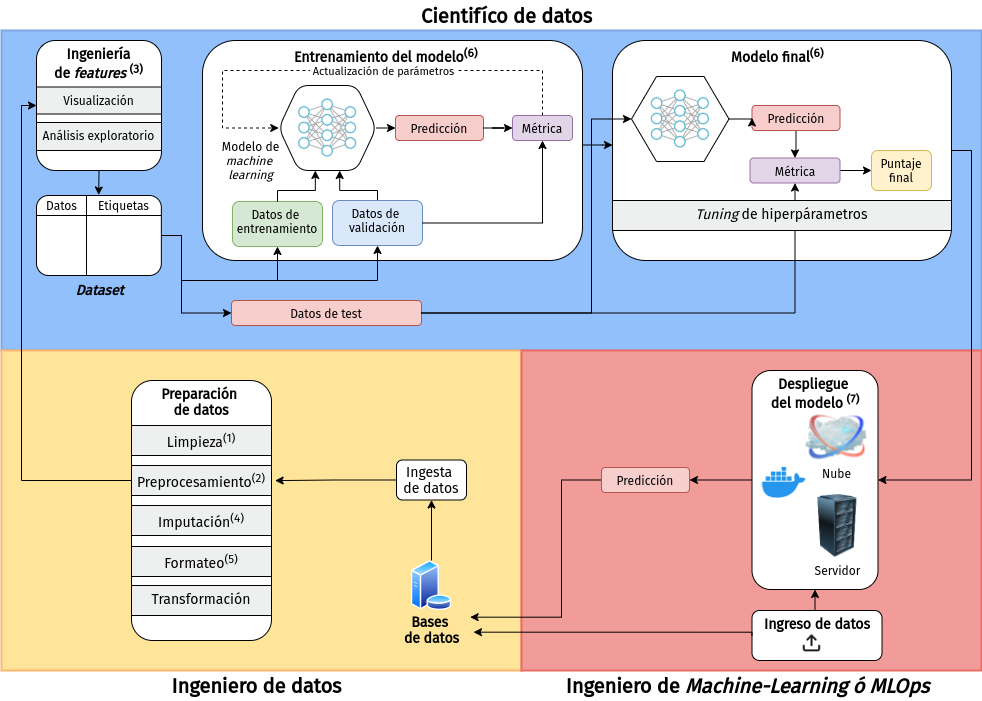
\includegraphics[width=1\textwidth]{ml-cycle.png}
		\caption{Arquitectura de un sistema de inteligencia artificial.}
		\label{fig:flowchartml.}
	\end{center}
\end{figure}

%No obstante para exponer el desarrollo de cada una de estas etapas es imprescindible elaborar un marco teórico que nos brinde contexto y herramientas para afrontar el problema a resolver.

\clearpage

\subsection{Objetivos}
\subsubsection{Objetivos principales}
Aplicar un modelo de \textit{Machine Learning} cuyo fin será el pronóstico de la cantidad de defectos graves de las unidades en la línea de producción de una planta automotriz.

\subsubsection{Objetivos secundarios}

\begin{itemize}
	\item Evaluar los diversos algoritmos disponibles de \textit{Machine Learning}, explorando todas las posibilidades en aras de identificar el modelo que mejor se adapte al problema a afrontar.
	      	      	      	
%	\item Analizar los principios fundamentales de las redes neuronales \textit{feedforward}, convolucionales y recurrentes, así como sus elementos, algoritmos y arquitecturas que posibilitan su funcionalidad. Explorar y reconocer fortalezas y debilidades de cada uno según el tipo de problema a afrontar.
	      	      	      	
	\item Establecer y evaluar la mejor configuración de parámetros para una determinada arquitectura de red con el fin de optimizar su desempeño.
	      	      	      	
%	\item Identificar, describir y clasificar las series temporales para evaluar su aplicación en la solución.
	      	      	      	
	\item Analizar la entropía de la serie de datos para determinar si es posible establecer una correlación.
	      	      	      	
	\item Examinar el problema a afrontar en su contexto, para así determinar los requerimientos del mismo. Posteriormente haciendo uso de las herramientas para manipulación de datos obtener un formato acorde de la serie temporal para alimentar los modelos.
	      	      	      	
\end{itemize}

\clearpage

\subsection{Requerimientos}
En ingeniería, los requerimientos se utilizan como datos de entrada en la etapa del diseño del producto. Establecen qué debe hacer el sistema, aunque no especifican la manera en que debe hacerlo. \citep{sommerville2015software}

Existen dos tipos de requerimientos:
\begin{itemize}[noitemsep, topsep=2pt]
	\item \textbf{Funcionales}: son enunciados acerca de servicios que el sistema debe brindar, su reacción a entradas particulares y comportamiento en situaciones particulares.
	\item \textbf{No funcionales}: no se refieren directamente a la funcionalidad del sistema sino a las propiedades que emergen de ella como la fiabilidad, la capacidad de almacenamiento, disponibilidad, etc. Suelen aplicarse al sistema como un todo, más que a características específicas del sistema.
\end{itemize}

\vspace{0.3cm}

Para especificar estos requerimientos se ejecutaron las siguientes etapas:
\begin{itemize}[topsep=2pt]
	\item \textbf{Entrevista}:  Se realizó una entrevista con el responsable del departamento Calidad Fabricación en la cuál se planteó la posibilidad de crear este sistema dado el potencial de los datos recabados por la usina. Esta propuesta fue aceptada y se elevó a los superiores para su aprobación debido a materia de confidencialidad.
	\item \textbf{Investigación del estado del arte}: Se profundizó en el conocimiento sobre las herramientas del campo de la ciencia de datos y \textit{machine-learning}. Esto incluyó el perfeccionamiento del uso de las librerías e investigación sobre algoritmos y modelos de inteligencia artificial, lo que permitió obtener una mejor perspectiva sobre el sistema a desarrollar al conocer las posibilidades y limitaciones del área.
	\item \textbf{Entrevista cerrada}: Se repitió la primer etapa pero teniendo en cuenta la información recabada en la etapa anterior. Se transmitió el conocimiento adquirido al responsable para alinear los objetivos propuestos, añadiendo nuevas consideraciones y descartando funcionalidades inviables.
\end{itemize}

\subsubsection{Requerimientos funcionales}
Los requerimientos del sistema han sido obtenidos en base al estudio teórico de los sistemas disponibles para lograr nuestro objetivo. Los mismos son presentados en el Cuadro~\ref{tab:functional-requirements}.

\begin{table}[H]
	\centering
	\begin{tabular}{p{0.07\linewidth} p{0.87\linewidth}}
		\hline
		\multicolumn{1}{c}{\textbf{ID}} & \multicolumn{1}{c}{\textbf{Descripción}}                                                                 \\ \hline
		RF1                             & El sistema deber tomar los datos desde las bases de datos de la compañía.                               \\
		RF2                             & El \textit{pipeline} de datos debe procesar los datos para entregarlos al modelo en un formato acorde.    \\
		RF3                             & El \textit{pipeline} de datos debe tolerar fallos en la entrada de datos soportando formatos imprevistos. \\
		RF4                             & El modelo debe guardar todas sus inferencias en la base de datos para revisión de rendimiento.           \\
		RF5                             & El modelo debe recibir y entregar un flujo continuo de datos en tiempo real.                              \\
		RF6                             & El sistema debe permitir un reporte que se crea dentro del \textit{pipeline}.                             \\
		RF7                             & El sistema debe proveer una API para ser consumida desde una página web.                                 \\ \hline
	\end{tabular}
	\caption{Requerimientos funcionales.}
	\label{tab:functional-requirements}
\end{table}

\subsubsection{Requerimientos no funcionales}
Estos fueron especificados en conjunto con el director del Proyecto Integrador y acordados en la entrevista final con el responsable de la fábrica.

\begin{table}[H]
	\centering
	\begin{tabular}{p{0.07\linewidth} p{0.87\linewidth}}
		\hline
		\multicolumn{1}{c}{\textbf{ID}} & \multicolumn{1}{c}{\textbf{Descripción}}                                                                                         \\ \hline
		RNF1                            & Optimizar el tiempo de respuesta del \textit{pipeline} para evitar cuello de botella.                                             \\
		RNF2                            & Diseñar pruebas para corroborar fiabilidad del sistema.                                                                          \\
		RNF3                            & El sistema será desarrollado enteramente en un lenguaje que facilite la integración entre los diversos componentes del sistema. \\
		RNF4                            & El modelo deberá lograr un rendimiento satisfactorio mínimo (65\%$\leq$precisión).                                             \\
		RNF5                            & El sistema debe ser accesible para cualquier usuario en la fábrica que lo necesite.                                              \\
		RNF6                            & El sistema utilizará un \textit{framework} de \textit{machine-learning} con respaldo de la comunidad para obtener soporte.       \\
		RNF7                            & El sistema debe proveer una API para ser consumida desde una página web.                                                         \\ \hline
	\end{tabular}
	\caption{Requerimientos no funcionales.}
	\label{tab:non-functional-requirements}
\end{table}

\subsection{Riesgos}
Un riesgo se define como un evento o condición incierta que en caso de ocurrir tendrá consecuencia sobre al menos uno de los requerimientos del proyecto.
\subsubsection{Tipos de riesgos} \label{sec:risk-types}
Se pueden identificar varios tipos de riesgos en un sistema como el que se intenta desarrollar.
\begin{itemize}[noitemsep, topsep=2pt]
	\item \textbf{Riesgos de proyecto} (P): amenazan la planificación del proyecto, principalmente los aspectos relacionados al tiempo.
	\item \textbf{Riesgos técnicos} (T): repercuten directamente en la calidad del producto.
	\item \textbf{Riesgos de negocio} (N): comprometen la viabilidad del proyecto.
\end{itemize}

\subsection{Gestión de riesgos}
Es un enfoque estructurado para \textit{manejar} la incertidumbre ante amenazas a través de una secuencia de actividades que tienen como objetivo reducir los efectos negativos de los riesgos ya sea evadiendolos si es posible o aceptando las consecuencias en el peor de los casos. 

Las etapas que lo componen son las siguientes:
\begin{enumerate}[noitemsep, topsep=2pt]
	\item \textbf{Identificación de riesgos}.
	\item \textbf{Análisis de riesgos}.
	\item \textbf{Selección de riesgos}.
	\item \textbf{Elaboración de planes de riesgos}.
\end{enumerate}

\subsubsection{Identificación de los riesgos}
Se realizó en base al conocimiento existente sobre los datos y el modelo a desarrollar. Los riesgos fueron clasificados según lo visto en la sección~\ref{sec:risk-types}.

\begin{table}[H]
	\centering
	\begin{tabular}{p{0.3\linewidth} p{0.63\linewidth}}
		\hline
		\multicolumn{1}{c}{\textbf{Riesgo}}            &   
		\multicolumn{1}{c}{\textbf{Descripción}} \\ \hline
		Aumento del tiempo de desarrollo del proyecto. &   
		Que el producto a realizar sea de mayor magnitud a la estimada, llevando a mayores tiempos de desarrollo. \\
		Planificación optimista.                      &   
		Se planifica el proyecto en base a criterios de situaciones óptimas o ideales en las que no se presentan problemas graves. \\ \hline
	\end{tabular}
	\caption{Identificación de riesgos de proyecto.}
	\label{tab:project-risks}
\end{table}

\begin{table}[H]
	\centering
	\begin{tabular}{p{0.3\linewidth} p{0.63\linewidth}}
		\hline
		\multicolumn{1}{c}{\textbf{Riesgo}}                             &   
		\multicolumn{1}{c}{\textbf{Descripción}} \\ \hline
		Desestimación de inversión.                                   &   
		La compañía una vez que el desarrollo del producto se encuentre en etapa avanzada hará un análisis de costes y beneficios para decidir la culminación total del proyecto. \\
		Falta de personal técnico para conformar equipo de desarrollo. &   
		La compañía debe evaluar el despliegue técnico que necesita el modelo ya que la naturaleza de este es transversal a varios sistemas de la fábrica y su implementación requiere de un equipo de desarrollo especializado. \\ \hline
	\end{tabular}
	\caption{Identificación de riesgos de negocio.}
	\label{tab:business-risks}
\end{table}

\begin{table}[H]
	\centering
	\begin{tabular}{p{0.3\linewidth} p{0.63\linewidth}}
		\hline
		\multicolumn{1}{c}{\textbf{Riesgo}}                                                                                  &   
		\multicolumn{1}{c}{\textbf{Descripción}} \\ \hline
		Arquitectura de sistemas de la organización no apta para el despliegue del modelo.                                  &   
		Muchos de los sistemas utilizados en la organización datan de largo tiempo e inclusive no reciben mantenimiento activo. Por tanto es necesario revisar la factibilidad de la integración del producto con estos sistemas y la obtención de los datos necesarios. \\
		Servidor con \textit{hardware} insuficiente para ejecutar el modelo.                                                 &   
		La compañía deberá evaluar la adquisición o alquiler de \textit{hardware} especifico y necesario para el entrenamiento e inferencia del modelo. \\
		Incapacidad de acceso en tiempo real a las bases de datos. &   
		Se deben actualizar las bases de datos actuales (actualmente bajo el modelo SAP) para proveer los datos al modelo en tiempo real para su inferencia. \\
		Pérdida del modelo entrenado por situación imprevista                                                              &   
		En ciertas ocasiones los modelos son entrenados por largos intervalos de tiempo para luego obtener los reportes y sus pesos. Sin embargo a veces surgen situaciones imprevistas que corrompen el código con el tiempo de ejecución avanzado provocando la pérdida de estos datos. \\ \hline
	\end{tabular}
	\caption{Identificación de riesgos técnicos.}
	\label{tab:technical-risks}
\end{table}

\clearpage

\subsubsection{Análisis de riesgos}
No es posible tratar todos los riesgos existentes por tanto se procederá a cuantificar los mismos para compararlos y priorizar aquellos que se consideren con mayor relevancia para su tratamiento. 

La posibilidad de ocurrencia se medirá de forma continua entre 0 y 1, donde 0 significa que es prácticamente imposible que ocurra y 1 es muy probable. Por otro lado, el impacto se medirá en una escala discreta entre 1 y 4 cuyos niveles representan:
\begin{enumerate}[noitemsep, topsep=2pt]
	\item Insignificante.
	\item Tolerable.
	\item Importante.
	\item Muy grave.
\end{enumerate}

La exposición $(E)$ es el producto entre la probabilidad $(P)$ y el impacto del riesgo $(R)$, representando con este valor la gravedad del mismo.

$$ E = PI $$

\begin{table}[H]
	\centering
	\begin{tabular}{p{0.67\linewidth} c c c c}
		\hline
		\multicolumn{1}{c}{\textbf{Riesgos}} &
		\multicolumn{1}{c}{\textbf{Tipo}} &
		\multicolumn{1}{c}{\textbf{P}} &
		\multicolumn{1}{c}{\textbf{I}} &
		\multicolumn{1}{c}{\textbf{E}} \\ \hline
		Aumento de la complejidad del proyecto.                         & P & 0,4 & 2 & 0,8 \\
		Planificación optimista.                                       & P & 0,5 & 3 & 1,5 \\
		Desestimación de inversión.                                   & N & 0,8 & 3 & 2,4 \\
		Falta de personal técnico para conformar equipo de desarrollo. & N & 0,6 & 3 & 1,8 \\
		Arquitectura de sistemas de la organización no apta para el despliegue del modelo. &
		T &
		0,9 &
		3 &
		\textbf{2,7} \\
		Servidor con hardware insuficiente para ejecutar el modelo.     & T & 0,7 & 3 & 2,1 \\
		Se debe acceder a las bases de datos a través de un protocolo que permite la transferencia de datos en tiempo real. &
		T &
		0,7 &
		4 &
		\textbf{2,8} \\
		Pérdida del modelo entrenado por situación imprevista         & T & 0,6 & 2 & 1,2 \\ \hline
	\end{tabular}
	\caption{Riesgos.}
	\label{tab:risk-table}
\end{table}

\clearpage

\subsubsection{Selección de riesgos}
Para esta tarea se decidió utilizar el principio de Pareto \citep{pareto}, el cual establece que de forma general, el 20\% del esfuerzo produce el 80\% de los resultados. O dicho de otra manera: el 80\% de las consecuencias provienen del 20\% de las causas, así  le daremos prioridad al conjunto de riesgos de mayor exposición para mitigar sus efectos. El 20\% de los 8 riesgos mostrados en el cuadro~\ref{tab:risk-table} es 1.6, el cual redondearemos a 2.

\subsubsection{Elaboración de planes de riesgos}
Para esta tarea realizaremos dos tipos de planes.
\begin{itemize}[noitemsep]
	\item \textbf{Plan de mitigación}: su objetivo es reducir la probabilidad de ocurrencia del riesgo o el impacto que el mismo puede provocar.
	\item \textbf{Plan de contingencia}: está comprendido por acciones que se deberán realizar solamente si el riesgo se presenta.	
\end{itemize}

Los dos riesgos principales son de tipo técnico, esto en gran parte se debe a la escasa actualización de los sistemas de la empresa. Esto provoca un gran déficit tecnológico que vulnera las oportunidades de soluciones informáticas en diversas áreas de la fábrica. No obstante, en el cuadro~\ref{tab:risks-plans} definimos planes de mitigación y contingencia para cada uno de estos riesgos.

\begin{table}[H]
\centering
\begin{tabular}{p{0.2\linewidth} p{0.35\linewidth} p{0.35\linewidth}}
\hline
\multicolumn{1}{c}{\textbf{Riesgo}} &
  \multicolumn{1}{c}{\textbf{Plan de mitigación}} &
  \multicolumn{1}{c}{\textbf{Plan de contingencia}} \\ \hline
Arquitectura de sistemas de la organización no apta para el despliegue del modelo. &
  Contactarse desde una etapa temprana con el departamento de informática de la empresa para determinar el estado actual de los sistemas. En caso que sea realizable la implementación podemos trabajar desde etapas tempranas teniendo en cuenta los sistemas, de este modo se ahorran tiempos al momento de la integración. &
  Realizar un reporte detallado de costos y beneficios del proyecto para que los directivos analicen de forma más organizada la información para tomar la decisión. Esto incluiría diversos beneficios como la actualización de varios sistemas de la fábrica que no reciben soporte ya y por tanto tienen un rendimiento reducido además de presentar vulnerabilidades. \\
Incapacidad de acceso en tiempo real a las bases de datos. &
  Comunicarse con el departamento de informática con el objetivo de obtener soporte oficial de la empresa creadora del sistema de base de datos. La idea es explorar la posibilidad de crear un protocolo que permita conectar nuestro sistema con la base de datos en tiempo real. &
  Proponer la migración o duplicación de los datos necesarios a una base de datos relacional que permita realizar consultas en tiempo real. \\ \hline
\end{tabular}
\caption{Elaboración de planes de riesgo.}
\label{tab:risks-plans}
\end{table}

\clearpage

\section{Inteligencia Artificial}

\begin{quote}
	La \textit{Inteligencia Artificial (Artificial Intelligence)} se define como el estudio de los "agentes inteligentes", i.e. cualquier dispositivo que perciba su entorno y tome medidas que maximicen sus posibilidades de lograr con éxito sus objetivos.
	  
	\hfill \citet{poole1998}
\end{quote}

Esta definición nos da la idea de que la IA es un sistema reactivo, que reacciona a cambios externos y actúa en consecuencia.

\subsection{Aprendizaje automático} \label{machinelearning}

\begin{quote}
	El \textit{aprendizaje automático (Machine Learning)} es el estudio científico de algoritmos y modelos estadísticos que los sistemas informáticos utilizan para realizar una tarea específica sin utilizar instrucciones explícitas, sino que se basan en patrones e inferencia. Es visto como un subcampo de inteligencia artificial. Los algoritmos de aprendizaje automático crean un modelo matemático basado en datos de muestra, conocidos como "datos de entrenamiento", para hacer predicciones o decisiones sin ser programado explícitamente para realizar la tarea.
	  
	\hfill \citet{bishop2006pattern}
\end{quote}

Es importante destacar la independencia del aprendizaje automático al momento de tomar decisiones a partir de los datos proporcionados sin intervención externa, es decir que no hay una especificación de reglas que dictan cómo deben ser tomadas estas decisiones. A su vez, los modelos obtenidos a partir de los algoritmos de \textit{Machine Learning} deben tener la capacidad de predecir a partir de nuevos datos, nunca antes procesados por el modelo, a esto se lo conoce como \textbf{generalización}. 

En el anexo del proyecto integrador se ha realizado un profundo análisis de los métodos y algoritmos más utilizados en el campo de la Inteligencia Artificial.
%
%\subsection{Preprocesamiento} \label{preprocessing}
%Este punto es vital para cualquier proyecto que utiliza algoritmos de \textit{Machine Learning}, debido a que los datos incluidos en los conjuntos conocidos como \textit{datasets}, no suelen presentarse en condiciones para obtener el óptimo rendimiento de los algoritmos de aprendizaje. Estos datos suelen estar desbalanceados, con faltantes o ruidosos, entre otras cuestiones. 
%
%Una vez obtenido el \textit{dataset} de entrada es primordial investigar, limpiar y transformar los datos con diversas técnicas. Una vez que los datos estén en condiciones procedemos al entrenamiento de nuestro modelo, con el propósito de lograr un desempeño óptimo.
%
%Para lograr este objetivo se aplican técnicas tales como normalización, reescalado, reducción de dimensionalidad, discretización, tratamiento de anomalías y \textit{outliers}.
		
		\section{Procesamiento de datos}
						
		\subsection{Origen de los datos}
		Los datos recabados provienen de la línea de fabricación de vehículos utilitarios en una fábrica de automotores, en la cual se utiliza un sistema de diversas auditorias para identificar defectos.
						
		\subsubsection{Organización de la usina}
		La fábrica está compuesta de departamentos, talleres y unidades de trabajo en ese orden jerárquico. A continuación listaremos los departamentos:
						
		\begin{itemize}[noitemsep, topsep=2pt]
			\item Calidad (\texttt{CALI})
			\item Embutición (\texttt{EMBU})
			\item Ingeniería (\texttt{DLI})
			\item Logística (\texttt{SQF})
			\item Montaje (\texttt{MONT})
			\item Pintura (\texttt{PINT})
			\item Soldadura (\texttt{SOLD})
			\item División de abastecimiento de piezas (\texttt{DIVD})
		\end{itemize}
						
		La línea de fabricación consta de 4 departamentos que intervienen directamente en el ensamblaje del vehículo:
						
		\texttt{EMBU -> SOLD -> PINT -> MONT}
						
		Los demás departamentos son una parte vital de la producción pero intervienen indirectamente, y \texttt{CALI} se encarga de verificar los defectos con mayor recurrencia de los departamentos. La figura~\ref{fig:dptodiagram} nos esclarece esta idea.
						
		\begin{figure}[H]
			\begin{center}				
				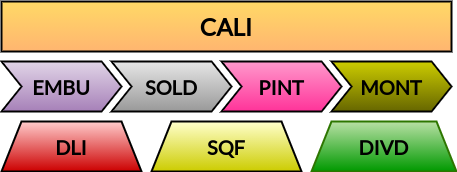
\includegraphics[width=0.6\textwidth]{usina.png}
				\caption{Diagrama de departamentos de la fábrica.}
				\label{fig:dptodiagram}
			\end{center}
		\end{figure}
						
		Cabe destacar a su vez que cada departamento posee talleres, que a su vez poseen unidades de trabajo obteniendo una estructura jerárquica de tipo árbol.
						
		\subsubsection{Nomenclatura de defectos}
						
		Un defecto (\texttt{DEF}) en su esencia se compone de un elemento (\texttt{ELE}), un incidente (\texttt{INC}) y opcionalmente una localización (\texttt{LOC}).
						
		\texttt{DEF = ELE + INC + LOC}
						
		Tanto \texttt{ELE} como \texttt{INC} están definido inequívocamente por un código de 4 caracteres mientras que \texttt{LOC} puede variar, lo que lleva a que un defecto posea al menos 8 caracteres.
						
		\subsubsection{Gravedad}
		Además los defectos se categorizan según la gravedad (\texttt{GVD}) del mismo en:
		\begin{itemize}[noitemsep, topsep=2pt]
			\item \texttt{V1}: graves.
			\item \texttt{V2}: leves.
			\item \texttt{V3}: imperceptibles (para nuestro análisis serán descartados).
		\end{itemize}
						
		\subsubsection{Tipo}
		A su vez los defectos están categorizados por familia o tipo de defectos:
						
		\begin{itemize}[noitemsep, topsep=2pt]
			\item \texttt{APR}: aprietes.
			\item \texttt{ASP}: aspecto.
			\item \texttt{DGRC}: degradaciones.
			\item \texttt{ELEC}: eléctrico.
			\item \texttt{ESTQ}: estanqueidad.
			\item \texttt{FCIO}: funcionamiento.
			\item \texttt{FLDS}: fluidos.
			\item \texttt{FTES}: faltantes.
			\item \texttt{GMTR}: geometría.
			\item \texttt{MOP}: modo operatorio.
			\item \texttt{NCON}: no conforme.
			\item \texttt{RDOS}: ruidos.
		\end{itemize}
						
		\subsubsection{Puntos de reconocimiento de defectos} \label{ptocptj}
		Los defectos son detectados en diversos puntos de captaje que pueden definir (o no) a que departamento o taller pertenece el defecto con un doble objetivo. En primer lugar para que los vehículos que ya poseen el defecto detectado sean derivados a puntos de retoque para ser reparados. Y en segundo para analizar y ejecutar diversas estrategias con el fin atacar el problema raíz para así erradicar el defecto.
						
		\clearpage				
						
		Los defectos detectados provienen de las siguientes fuentes de datos:
		\begin{itemize}[noitemsep, topsep=2pt]
			\item \textbf{Defectos por unidad} (\texttt{DPU}): los defectos encontrados en los puntos de reconocimiento a lo largo de toda la línea de producción.
			\item \textbf{Carrocería pintura-soldadura} (\texttt{CAPS}): se realiza una auditoria al final de la línea de pintura sobre una muestra de carrocerías.
			\item \textbf{Plan estático-dinámico} (\texttt{PESD}): una vez finalizado el proceso de fabricación del vehículo, se le realizan pruebas de estanqueidad, prueba de manejo, entre otros con objeto de encontrar defectos que en línea no sería posible.
			\item \texttt{SAVES}: Auditoria de 5 minutos de una muestra aleatoria de vehículos en línea final.
		\end{itemize}
						
		Sin embargo solo obtenemos datos a partir de los puntos de captaje de \texttt{SOLD} dado que en \texttt{EMBU} las partes aún no poseen un identificador único del vehículo.
						
		\subsection{Ingeniería de datos}
		Es vital realizar el procesamiento de los datos para alimentar el modelo con los datos en un formato acorde, lo que se conoce en la industria como \textbf{ingeniería de datos}.
						
		Para ello se ha divido la tarea en las etapas o \textit{stages} que se muestran en la figura \ref{fig:dataproc}.
						
		\begin{figure}[H]
			\begin{center}				
				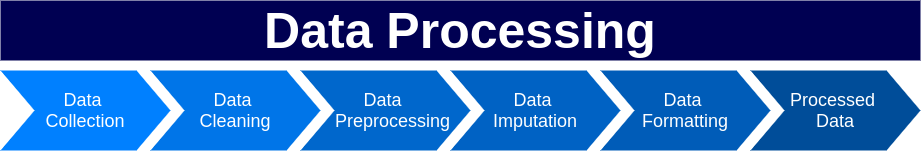
\includegraphics[width=1\textwidth]{dataproc.png}
				\caption{Procesamiento de datos segmentado en etapas.}
				\label{fig:dataproc}
			\end{center}
		\end{figure}
						
		En el campo de ciencia de datos la comunidad ha consensuado de facto que el estándar es utilizar como entorno de trabajo \texttt{Jupyter-Notebook}, que soporta \texttt{Python} como lenguaje de programación. Existen otros lenguajes reconocidos como \texttt{R} pero poseen mayor difusión en comunidades académicas.
						
		Las librerías que serán parte del proyecto son las siguientes: 
		\begin{itemize}[noitemsep, topsep=2pt]
			\item \texttt{Pandas}: manejo de tablas y datos.
			\item \texttt{Numpy}: operaciones matriciales.
			\item \texttt{Matplotlib}, \texttt{Seaborn}: visualización de datos.
		\end{itemize}
						
		\subsubsection{Recolección de datos}
						
		Etapa de búsqueda y recolección de los datos que alimentarán el modelo. En nuestro caso se dividió en recolectar en la organización los datos de defectos, que fueron obtenidos desde 4 auditorias diferentes que fueron presentadas en \ref{ptocptj}.
						
		\subsubsection{\href{https://github.com/GeraCollante/tesis-icomp-machinelearning/blob/main/DataCleaning.ipynb}{\color{blue}Limpieza de datos}} \label{DataCleaning}
		Consiste en inspeccionar los datos obtenidos en búsqueda de posibles errores o datos que quizás es posible obtener pero por diversas razones se han perdido y debemos intentar recuperar.
						
		Ambos casos sucedieron, por tanto se procedió a recuperar los datos cuando fue posible, y en los que no se procedió al descarte debido a que no eran útiles para la tarea.
						
		\subsubsection{\href{https://github.com/GeraCollante/tesis-icomp-machinelearning/blob/main/DataPreproccesing.ipynb}{\color{blue}Preprocesamiento de datos}} \label{DataPreprocessing}
		En este punto es donde debemos prestar atención a los detalles al inspeccionar nuestro \textit{dataset}.
						
		En primer lugar se realizó una homogeneización de los datos, \textit{i.e.} quizás el mismo dato se puede estar refiriendo a lo mismo pero tienen \textit{tags} diferentes, por tanto es necesario revisar los datos columna por columna. Esto sucedió debido a que provenir los datos de diversas fuentes cada una tenía una forma de nombrarlos. 
						
		Posteriormente fue necesaria la detección de incongruencias, advirtiendo inconvenientes tales como departamentos inexistentes. Además todos los defectos que no hayan sido catalogados en el campo \texttt{GVD} pasaron a ser \texttt{V2}.
						
		Debido a la estructura jerárquica de la usina, si tenemos definido la UET a la que pertenece el defecto, escalando hacía arriba podemos obtener el taller y el departamento correspondiente. Esta operación se realizó para todo el \textit{dataset}.
						
		Una vez realizadas estas operaciones \textit{dataset} se encuentra en condiciones para su análisis.
						
		\subsubsection{\href{https://github.com/GeraCollante/tesis-icomp-machinelearning/blob/main/DataPlottingAndAnalysis.ipynb}{\color{blue}Análisis y visualización de datos}}\label{AnalysisVisualization}
		Para obtener una perspectiva más amplia del problema a tratar es conveniente analizar los datos disponibles. El \textit{dataset} se compone de $229934$ filas que cada una representa un defecto y 17 columnas.
						
		\clearpage				
						
		Algunas estadísticas \textit{grosso modo}, que podemos obtener:
						
		\begin{itemize}[noitemsep, topsep=2pt]
			\item 10780 vehículos fueron fabricados durante 2020.
			\item 5224 defectos diferentes fueron registrados en el sistema.
			\item Se registran en promedio 19,6 defectos por vehículo.
		\end{itemize}
						
		Si verificamos el origen de los datos nos percataremos que casi la totalidad de ellos provienen de \texttt{DPU}, disputándose el pequeño margen restante \texttt{PESD}, \texttt{CAPS} y \texttt{SAVES}.
						
		\begin{figure}[H]
			\begin{center}				
				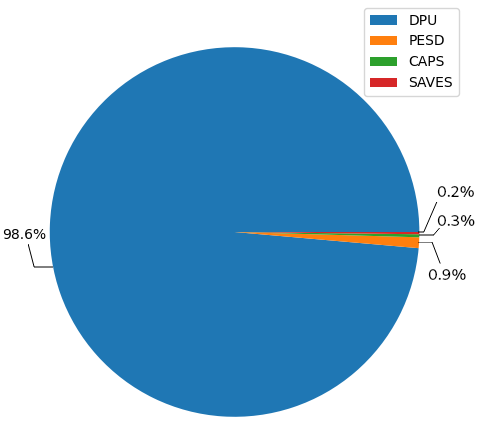
\includegraphics[width=0.45\textwidth]{audidist.png}
				\caption{Distribución de los defectos según \texttt{AUDI}.}
				\label{fig:distaudi}
			\end{center}
		\end{figure}
						
		No obstante, no se debe perder el propósito el cual es el pronostico de la cantidad de defectos graves que ocurrirán en función a todos los defectos registrados con anterioridad. En la fig.~\ref{fig:distgvddpto} observamos que la gran mayoría de defectos registrados son \texttt{V2} lo que podría ser útil para nuestro modelo.
						
		\begin{figure}[H]
			\begin{center}				
				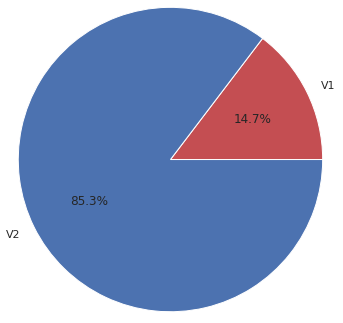
\includegraphics[width=0.40\textwidth]{tesis_51.png}
				\caption{Distribución de los defectos según gravedad.}
				\label{fig:distgvd}
			\end{center}
		\end{figure}
						
		La fig.~\ref{fig:distgvddpto} nos muestra que los defectos principalmente ocurren en 3: \texttt{PINT}, \texttt{SOLD} y \texttt{MONT}, un poco más atrás en la participación está \texttt{SQF}.
						
		\begin{figure}[H]
			\begin{center}				
				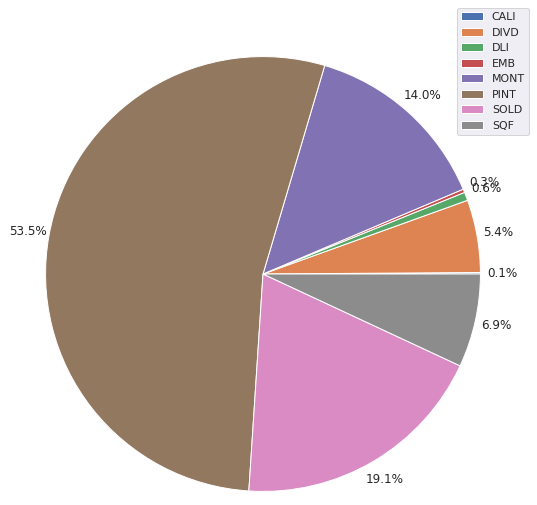
\includegraphics[width=0.56\textwidth]{tesis_53.png}
				\caption{Distribución de los defectos por \texttt{DPTO}.}
				\label{fig:distgvddpto}
			\end{center}
		\end{figure}
						
		La fig.~\ref{fig:distgvdtype} resume que casi 7 decimos de los defectos totales son de tipo \texttt{ASP}, seguido muy por detrás por \texttt{DGRC} y en tercer lugar los de \texttt{MOP}.
						
		\begin{figure}[H]
			\begin{center}				
				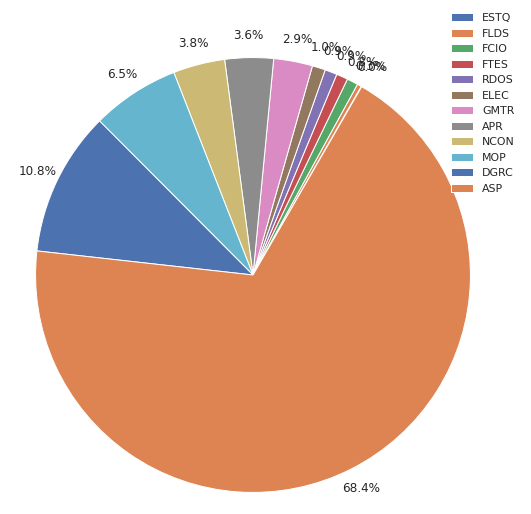
\includegraphics[width=0.56\textwidth]{tesis_55.png}
				\caption{Distribución de los defectos por \texttt{TIPO}.}
				\label{fig:distgvdtype}
			\end{center}
		\end{figure}
						
		Mediante un mapa de calor (fig.~\ref{fig:heatmapdptotype}) se cruzaron las características \texttt{TIPO} y \texttt{DPTO}. Advertimos una cierta correlación entre algunos tipos de defectos y los departamentos, a tal punto que en algunos departamentos ni siquiera existen determinados tipos de defectos. Sería beneficioso que el modelo pueda aprender esta característica para maximizar sus posibilidades.
						
		\begin{figure}[H]
			\begin{center}
				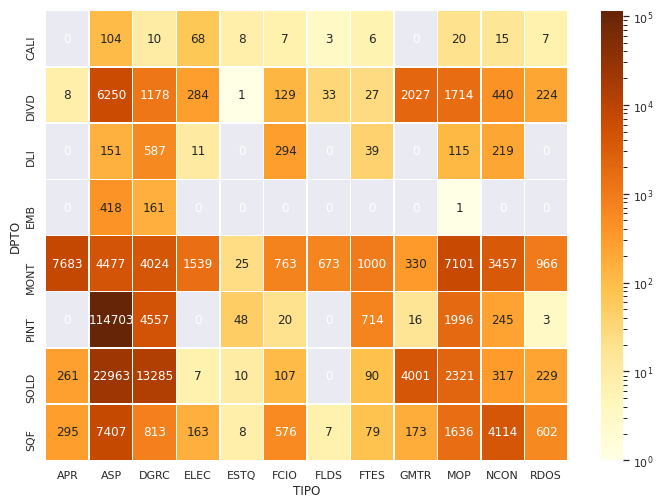
\includegraphics[width=1\textwidth]{tesis_56.png}
				\caption{Cantidad de defectos cruzando \texttt{DPTO} y \texttt{TIPO}.}
				\label{fig:heatmapdptotype}
			\end{center}
		\end{figure}
						
		Pese a esto no se debe creer que aunque una combinación tenga una gran cantidad de defectos, la mayoría de estos serán \texttt{V1}. La fig.~\ref{fig:heatmapfractionv1} nos muestra la densidad de \texttt{V1} sobre el total de defectos, permitiéndonos establecer que determinadas combinaciones de \texttt{TIPO} y \texttt{DPTO} son más probables que sean \texttt{V1} (incluso algunas poseen valores considerablemente más altos que las demás).
						
		\begin{figure}[H]
			\begin{center}
				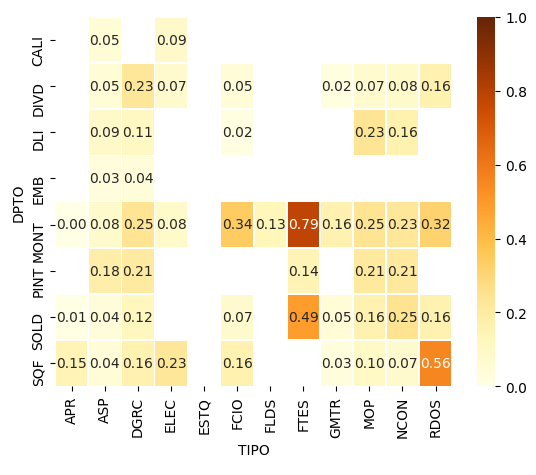
\includegraphics[width=0.8\textwidth]{tesis_58.png}
				\caption{Fracción de \texttt{V1} por cantidad de defectos.}
				\label{fig:heatmapfractionv1}
			\end{center}
		\end{figure}
						
		El análisis visual más revelador es el de la figura~\ref{fig:defectsperday}. El 19 de marzo de 2020 se decretó la cuarentena debido a la pandemia provocada por el virus \textit{SARS-CoV-2}, por tanto no se fabricaron vehículos. Los defectos registrados durante esa fecha y el reinicio de la producción en junio se deben a la recuperación de vehículos por retoques. Por esto para que el flujo de los datos hacía el modelo sea continuo solo se tomará desde junio a diciembre (6 meses).
						
		\begin{figure}[H]
			\begin{center}
				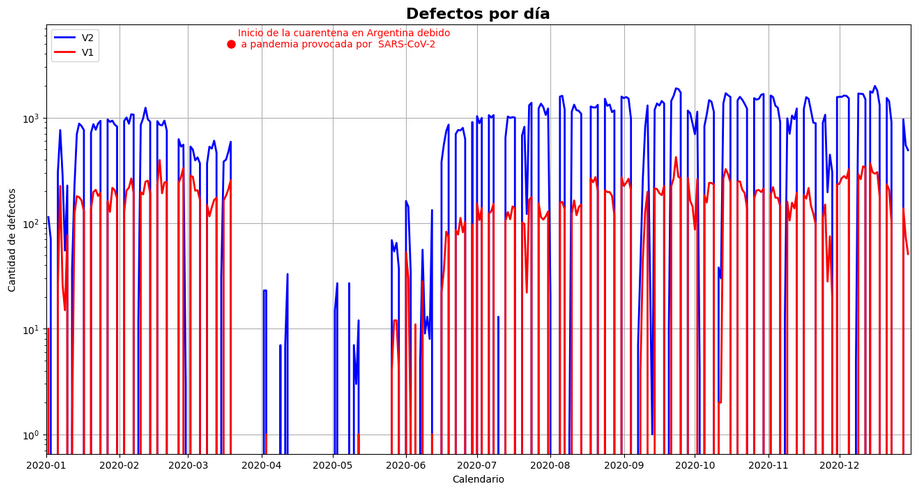
\includegraphics[width=1\textwidth]{tesis_64.png}
				\caption{Defectos diarios agrupados por \texttt{GVD}.}
				\label{fig:defectsperday}
			\end{center}
		\end{figure}
						
		Aún así, no podemos notar un patrón especifico debido al ruido, por consiguiente incrementamos la ventana de tiempo a una semana (fig.~\ref{fig:defectsperweek}). Afortunadamente para nuestro modelo (aunque la escala del eje de ordenadas es logarítmico) la cantidad de defectos \texttt{V2} sigue la curva de \texttt{V1} de forma muy similar. Esto es positivo ya que podemos intuir que existe una correlación entre los mismos del cúal nuestro modelo podrá obtener provecho.
						
		\begin{figure}[H]
			\begin{center}
				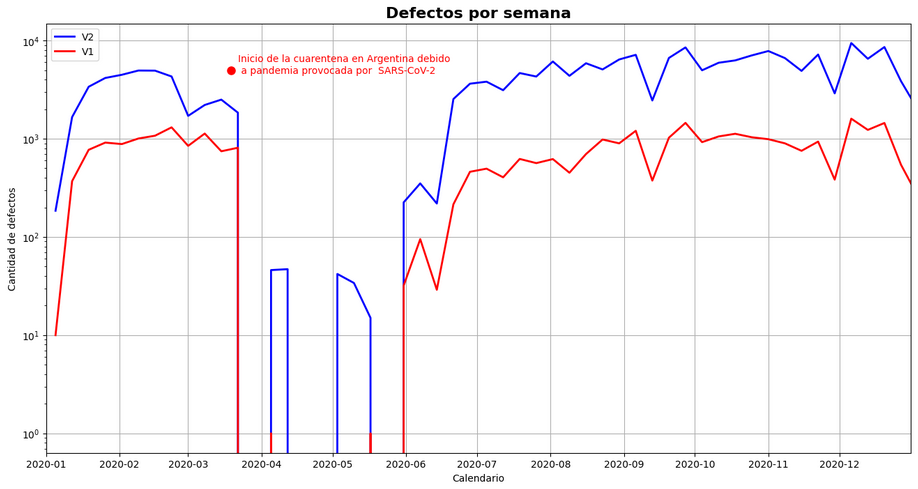
\includegraphics[width=1\textwidth]{tesis_63.png}
				\caption{Defectos semanales agrupados por \texttt{GVD}.}
				\label{fig:defectsperweek}
			\end{center}
		\end{figure}
						
		Si al gráfico anterior lo desglosamos por auditoria y gravedad (fig.~\ref{fig:defectsperaudigvdweek}) veremos que en las demás auditorias que no sean \texttt{DPU} no hay patrones claros definidos, una de las causas es la baja densidad de datos disponibles.
						
		\begin{figure}[H]
			\begin{center}
				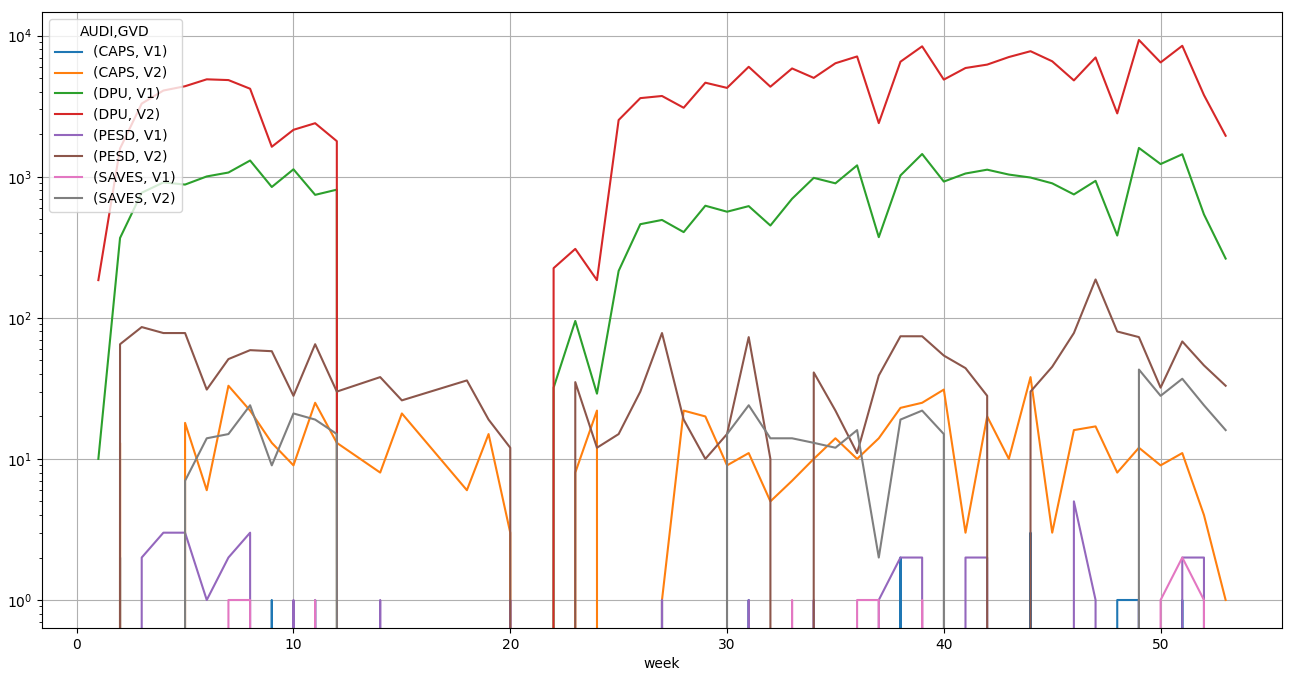
\includegraphics[width=1\textwidth]{audigvd.png}
				\caption{Defectos semanales agrupados por \texttt{AUDI}/\texttt{GVD}.}
				\label{fig:defectsperaudigvdweek}
			\end{center}
		\end{figure}
						
		\subsubsection{\href{https://github.com/GeraCollante/tesis-icomp-machinelearning/blob/main/DataImputation.ipynb}{\color{blue}Imputación de datos}}\label{DataImputation}
						 
		En estadística, la imputación es el proceso de reemplazar los datos faltantes (\textit{missing values}) con valores sustituidos. En nuestro \textit{dataset} tenemos 2 \textit{features} con faltantes, una es \texttt{UET} (lo que conlleva a faltantes de \texttt{DPTO} y \texttt{TALL}) y la otra es \texttt{TIPO}.
						
		Como se observa en la fig.~\ref{fig:missingvalue}, los datos faltantes no son demasiados, más precisamente $1052$ de \texttt{UET} y $1228$ de \texttt{TIPO}. Debido a la gran cantidad de datos disponibles podemos rellenar estos valores con algún algoritmo de \textit{Machine Learning} visto con anterioridad.
						
		\begin{figure}[H]
			\begin{center}
				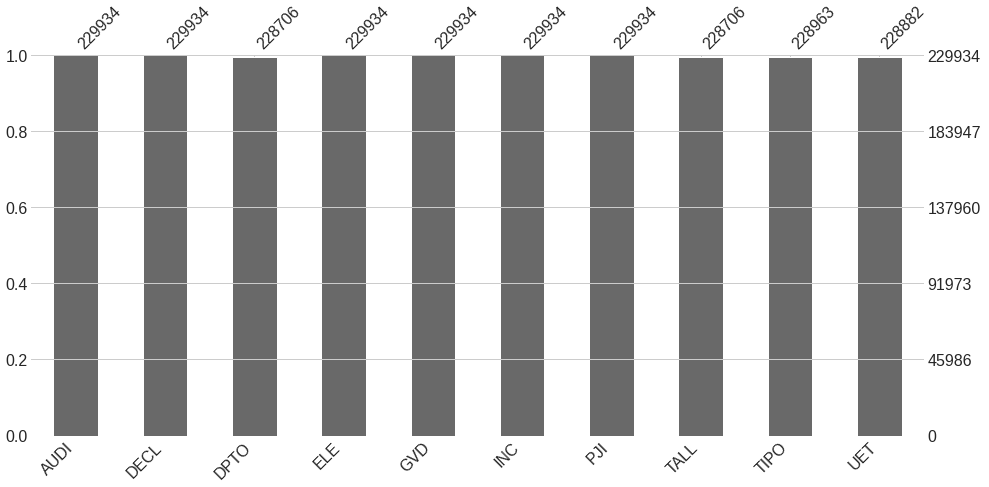
\includegraphics[width=1\textwidth]{tesis_66.png}
				\caption{Datos faltantes por \textit{feature}.}
				\label{fig:missingvalue}
			\end{center}
		\end{figure}
						
		\textbf{Matriz de correlación}
						
		En un \textit{dataset} con muchos atributos, el conjunto de valores de correlación entre pares de sus atributos forma una matriz que se denomina matriz de correlación.
						
		Existen varios métodos para calcular un valor de correlación. El más popular es el coeficiente de correlación de \textit{Pearson}. Sin embargo, debe notarse que mide solo la relación lineal entre dos variables. En otras palabras, es posible que no pueda revelar una relación no lineal. El valor de la correlación de \textit{Pearson} varía de $-1$ a $+1$, donde $\pm1$ describe una correlación positiva/negativa perfecta y $0$ significa que no hay correlación. \citep{corrmatrix}
						
		\clearpage				
						
		La matriz de correlación es una matriz simétrica con todos los elementos diagonales iguales a $+1$. Nos gustaría enfatizar que una matriz de correlación solo brinda información sobre la correlación y NO es una herramienta plenamente confiable para estudiar la causalidad. 
						
		\begin{figure}[H]
			\begin{center}
				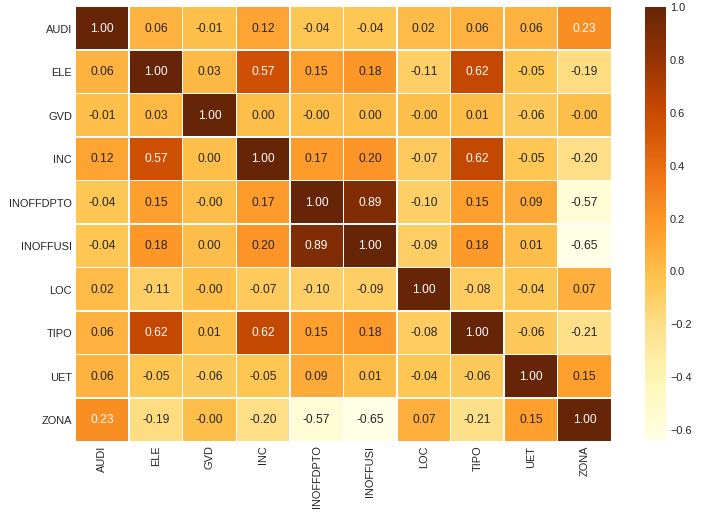
\includegraphics[width=1\textwidth]{corrmatrix.png}
				\caption{Matriz de correlación de nuestro \textit{dataset}.}
				\label{fig:corrmatrix}
			\end{center}
		\end{figure}
						
		En la fig.~\ref{fig:corrmatrix} pondremos atención sobre las dos \textit{features} que nos propusimos predecir.
						
		\begin{itemize}[noitemsep, topsep=2pt]
			\item \texttt{TIPO}: en este caso notamos que las features \texttt{ELE} y \texttt{INC}, tienen una relación notable con \texttt{TIPO}, por tanto esas serán utilizadas y el resto descartadas.
			\item \texttt{UET}: aquí las relaciones están mucho más difusas, por tanto usaremos \textit{features} que estén en las filas a las cuales queremos predecir su \texttt{UET}. Por tanto se seleccionó \texttt{ELE}, \texttt{INC}, \texttt{LOC}, \texttt{GVD} y \texttt{TIPO}.
		\end{itemize}
				
		\clearpage
						
		\textbf{\textit{Scikit-learn}}
						
		Dado que el proceso de imputación no es crítico, se optó por utilizar la librería \textit{sk-learn} (en lugar de redes neuronales) que nos provee de algoritmos ya implementados. Además nos permite a través de \textit{pipelines} realizar un preprocesamiento de los datos para posteriormente entrenar al modelo.
						
		Luego de revisar los valores faltantes se decidió utilizar como estimador diversos tipos de clasificadores para así seleccionar el de mejor rendimiento, para posteriormente rellenar los valores.
						
		Los siguientes clasificadores fueron seleccionados:
						
		\begin{itemize}[noitemsep, topsep=2pt]
			\item \textit{KNeighborsClassifier} \texttt{(KNC)}
			\item \textit{SGDClassifier} \texttt{(SGDC)}
			\item \textit{RidgeClassifier} \texttt{(RC)}
			\item \textit{LogisticRegression} \texttt{(LR)}
			\item \textit{XGBClassifier} \texttt{(XGBC)}
			\item \textit{DecisionTreeClassifier} \texttt{(DTC)}
			\item \textit{RandomForestClassifier} \texttt{(RFC)}
			\item \textit{BaggingClassifier} \texttt{(BC)}
		\end{itemize}
						
		\hfill
						
		\textbf{Estimación de la precisión del modelo}
						
		Para estimar la precisión de los modelos seleccionados se utilizó \textit{K-fold Cross-Validation} (\texttt{KFCV}) \citep{kfolds}.
						
		Una iteración de \texttt{KFCV} se realiza de la siguiente manera: 
						
		\begin{enumerate}[noitemsep, topsep=2pt]
			\item Se genera una permutación aleatoria del conjunto de muestra y se divide en $K$ subconjuntos (pliegues o \textit{folds}) de aproximadamente el mismo tamaño.
			\item De esos $K$ subconjuntos, un solo subconjunto se retiene como datos de validación para probar el modelo (este subconjunto se llama \textit{testset}), y los restantes $K-1$ subconjuntos juntos se utilizan como datos de entrenamiento (\textit{trainset}).
			\item Luego, se entrena un modelo en el \textit{trainset} y se evalúa su precisión en el \textit{testset}. 
			\item El entrenamiento y la evaluación del modelo se repiten $K$ veces, y cada uno de los $K$ subconjuntos se utiliza exactamente una vez como \textit{trainset}.
		\end{enumerate}
						
		En la fig.~\ref{fig:kfolds} se ejemplifica parte del proceso.
						
		\begin{figure}[H]
			\begin{center}
				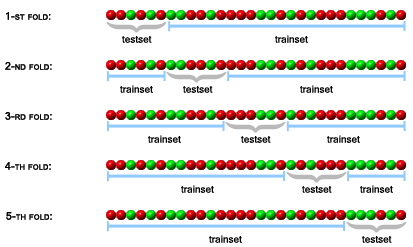
\includegraphics[width=1\textwidth]{tesis_67.png}
				\caption{Ejemplo de validación cruzada de 5 veces con 30 muestras.}
				\label{fig:kfolds}
			\end{center}
		\end{figure}
						
		La estimación de precisión resultante depende de la permutación aleatoria que se generó al comienzo del proceso, ya que afecta la forma en que se particiona el conjunto de muestras. 
						
		Por ello para obtener una estimación más exacta de la precisión, tiene sentido repetir la validación cruzada varias veces y tomar el promedio final después de cada iteración como estimación de precisión resultante.
						
		En nuestro caso debido a que todas las \textit{features} son de tipo categoría usamos la codificación \texttt{one-hot encoder}, como observamos en la fig.~\ref{fig:sklearn}.
						
		\begin{figure}[H]
			\begin{center}
				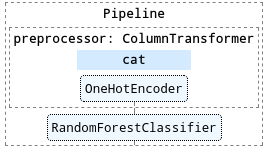
\includegraphics[width=0.45\textwidth]{tesis_74.png}
				\caption{\textit{Pipeline} de \textit{sklearn} para imputar datos.}
				\label{fig:sklearn}
			\end{center}
		\end{figure}
						
		\hfill
						
		\textbf{Selección de algoritmo}
						
		Al momento seleccionar un algoritmo para inferir los valores faltantes debemos tener en cuenta 3 criterios:
		\begin{itemize}
			\item \textbf{Tiempo de entrenamiento}: si nuestro \textit{dataset} crece y el poder de cómputo disponible es el mismo, es posible que este valor para un determinado algoritmo sea alto y por consiguiente inutilizable.
			\item \textbf{Tiempo de inferencia}: (también llamado latencia de predicción) es un valor importante ya que como mencionamos en la sección, nuestro modelo necesita un \textit{pipeline} de datos que lo alimente continuamente. Por tanto si el tiempo de inferencia es grande puede provocar un cuello de botella y eventualmente que el \textit{pipeline} se rompa.
			\item \textbf{Rendimiento}: es un valor importante, ya que en la medida que la inferencia de datos sea precisa nuestro modelo funcionará mejor.
		\end{itemize}
						
		\textbf{Predicción de \texttt{UET}}
						
		Teniendo en cuenta la matriz de correlación de la fig.~\ref{fig:corrmatrix} tomamos en consideración 5 \textit{features}, pero haremos un inspección más minuciosa de las mismas. Utilizando un \textit{miniset} (\textit{i.e.} una fracción de nuestro \textit{dataset}) se fueron probando diferentes \textit{features} para nuestro modelo (debido a que las pruebas requieren menor tiempo de cálculo y se supone que la muestra representa al menos la mayor parte del \textit{dataset}). Tener en cuenta que para que este enfoque funcione es necesario setear el \texttt{random-state} de las funciones con una \textit{seed} que es un número entero, el propósito de esto es quitar el componente de azar de los modelos y poder realizar las pruebas sobre los mismos datos.
						
		Los mejores rendimientos se obtenían con \texttt{ELE}, \texttt{INC} y \texttt{LOC}, ergo se descartó \texttt{GVD} y \texttt{TIPO}.
						
		\textbf{Cómputo de métricas para cada algoritmo}
		\begin{table}[H]
			\centering
			\begin{tabular}{lccc}
				\hline
				\multicolumn{1}{c}{\textbf{Algoritmo}} &
				\multicolumn{1}{c}{\textbf{Rendimiento $[\%]$}} &
				\multicolumn{1}{c}{\textbf{Inferencia $[ms]$}} &
				\multicolumn{1}{c}{\textbf{Entrenamiento $[s]$}} \\ 
				\hline
				\texttt{KNC}  & 73,59          & 31,75         & \textbf{0,59} \\
				\texttt{SGDC} & 72,56          & 6,82          & 14,99         \\
				\texttt{RC}   & 68,49          & 6,77          & 34,57         \\
				\texttt{LR}   & 74,20          & 6,64          & 89,74         \\
				\texttt{XGBC} & 72,23          & 9,82          & 305,77        \\
				\texttt{DTC}  & 77,22          & \textbf{6,23} & 4,60          \\
				\texttt{RFC}  & \textbf{77,66} & 20,91         & 262,14        \\
				\texttt{BC}   & 77,24          & 9,76          & 44,56         \\ 
				\hline
			\end{tabular}
			\caption{Parámetros de algoritmos para predicción de \texttt{TIPO}}
			\label{tab:tipo-parameters-algo}
		\end{table}
						
		\textbf{Rendimiento}
						
		En la fig.~\ref{fig:perfo_tipo_by_algo} notamos como \texttt{RFC}, \texttt{BC} y \texttt{DTC} son superiores a los demás algoritmos.
						
		\begin{figure}[H]
			\begin{center}
				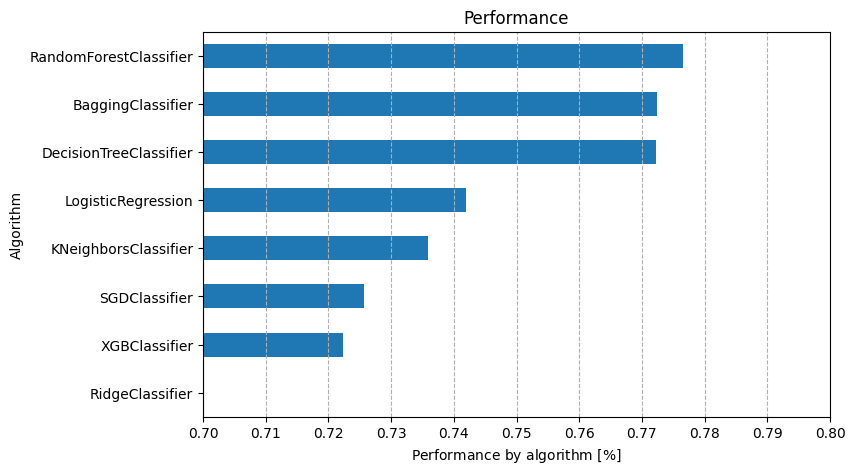
\includegraphics[width=0.9\textwidth]{perfo_tipo_by_algo.png}
				\caption{Rendimiento por algoritmo.}
				\label{fig:perfo_tipo_by_algo}
			\end{center}
		\end{figure}
						
		\textbf{Tiempo de entrenamiento}
						
		Hay resultados muy dispares entre los algoritmos, algunos como \texttt{DTC} son muy veloces mientras que otros como \texttt{RFC} o \texttt{XGBC} necesitan demasiado tiempo.
						
		\begin{figure}[H]
			\begin{center}
				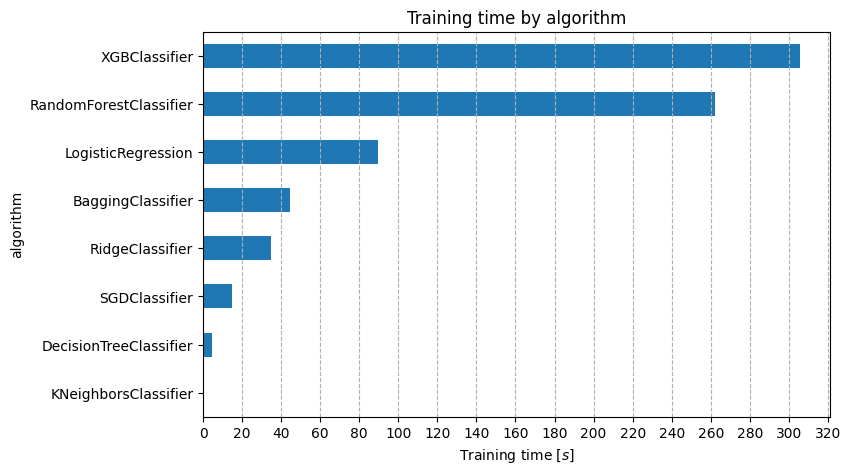
\includegraphics[width=0.9\textwidth]{training_time_tipo.png}
				\caption{Tiempo de entrenamiento por algoritmo.}
				\label{fig:training_time_tipo}
			\end{center}
		\end{figure}
						
		\textbf{Tiempo de inferencia}
						
		Se realizó inferencia atómica (\textit{i.e.} muestra por muestra, en vez de por loteo) sobre 10000 muestras recopilando los tiempos de cada algoritmo. Anacelicemos el gráfico de cajas expuesto en la fig.~\ref{fig:inference_time_tipo}. La gran mayoría de los algoritmos muestra tiempos cercanos a $5ms$, no obstante se pueden observar algunos \textit{outliers} que llegan a $20ms$. \texttt{KNC} tiene tiempos muy altos de inferencia sumado a una gran dispersión debido a que el cálculo de la distancia euclidiana puede llevar a mucho tiempo de cómputo. \texttt{RFC} por su parte tarda en promedio 5 veces más que los demás algoritmos, lo cual es una desventaja al momento de la decisión final.
						
		\begin{figure}[H]
			\begin{center}
				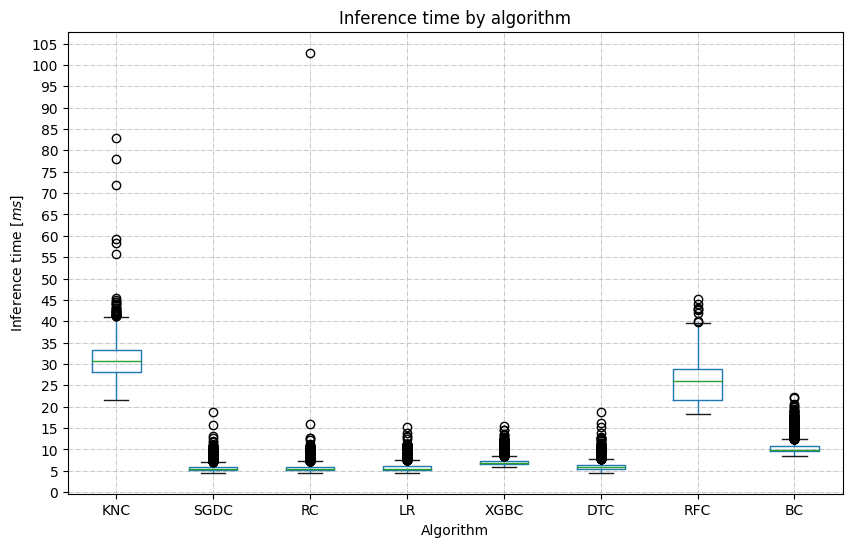
\includegraphics[width=0.9\textwidth]{inference_time_tipo.png}
				\caption{Tiempo de inferencia por algoritmo.}
				\label{fig:inference_time_tipo}
			\end{center}
		\end{figure}
						
		\textbf{Comparación visual de métricas}
						
		El gráfico de dispersión presentado en la fig.~\ref{fig:inference_training_perfo_tipo} es útil para seleccionar el mejor algoritmo ya que en el eje de abscisas está el rendimiento, en el eje de coordenadas el tiempo de inferencia y el tamaño del círculo se corresponde con el tiempo de entrenamiento. Por tanto el mejor algoritmo será el punto de menor tamaño que se encuentre más cercano a la esquina inferior derecha. 
						
		En consecuencia seleccionamos \texttt{DTC} para la imputación de datos de \texttt{TIPO}, ya que a pesar de tener menor rendimiento que \texttt{RFC} tiene mejores tiempos de inferencia y entrenamiento.
						
		\begin{figure}[H]
			\begin{center}
				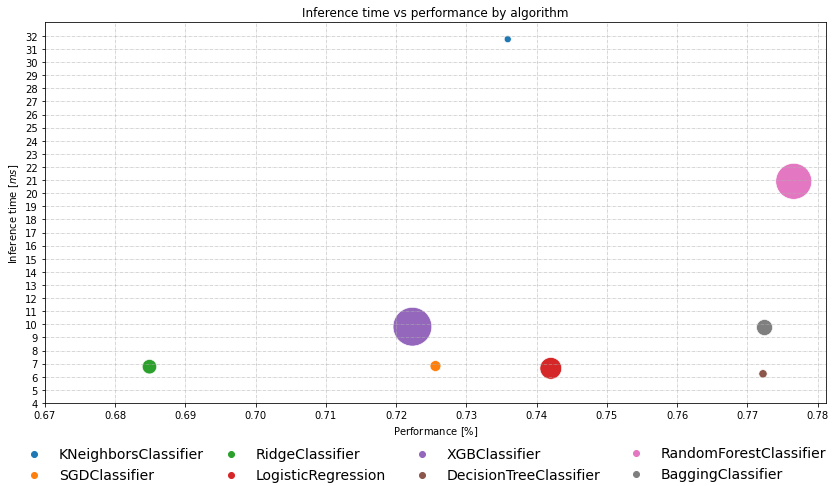
\includegraphics[width=1\textwidth]{inference_training_perfo_tipo.png}
				\caption{Gráfico de dispersión de métricas por algoritmo.}
				\label{fig:inference_training_perfo_tipo}
			\end{center}
		\end{figure}
						
		\textbf{Predicción de \texttt{UET}}
						
		Se realizará el mismo análisis aplicado a \texttt{TIPO}.
						
		\textbf{Cómputo de métricas para cada algoritmo}
						
		\begin{table}[H]
			\centering
			\begin{tabular}{lccc}
				\hline
				\multicolumn{1}{c}{\textbf{Algoritmo}} &
				\multicolumn{1}{c}{\textbf{Rendimiento $[\%]$}} &
				\multicolumn{1}{c}{\textbf{Inferencia $[ms]$}} &
				\multicolumn{1}{c}{\textbf{Entrenamiento $[s]$}} \\ 
				\hline
				\texttt{KNC}  & 97,37          & 28,26         & \textbf{0,74} \\
				\texttt{SGDC} & 98,95          & \textbf{5,38} & 3,63          \\
				\texttt{RC}   & 98,21          & 5,39          & 7,11          \\
				\texttt{LR}   & 99,06          & 5,40          & 29,22         \\
				\texttt{XGBC} & \textbf{99,61} & 6,44          & 55,65         \\
				\texttt{DTC}  & 99,02          & 5,58          & 4,04          \\
				\texttt{RFC}  & 98,99          & 19,20         & 64,65         \\
				\texttt{BC}   & 99,15          & 9,54          & 32,03         \\ 
				\hline
			\end{tabular}
			\caption{Parámetros de algoritmos para predicción de \texttt{TIPO}. Destacados los valores óptimos por columna.}
			\label{tab:tipo-parameters-algo}
		\end{table}		
						
		\clearpage				
						
		\textbf{Rendimiento}
						
		Existe un salto notable entre los rendimientos obtenidos para la predicción de \texttt{TIPO} con respecto a la de \texttt{UET}. 
				
		Sugerimos que una razón de esto se debe a la estructura de árbol que posee \texttt{UET} (recordemos que un departamento está compuesto por varios talleres que a su vez poseen múltiples \texttt{UET}s, lo que lleva a una cantidad única de etiquetas superior a la de \texttt{TIPO}). La mayoría de los algoritmos tienen desempeños similares, siendo el óptimo \texttt{BC}.
						
		\begin{figure}[H]
			\begin{center}
				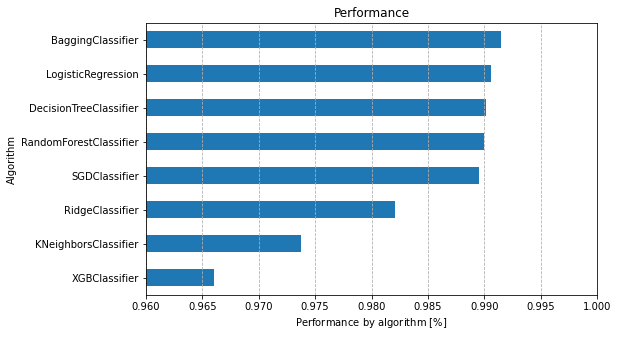
\includegraphics[width=0.9\textwidth]{perfo_uet_by_algo.png}
				\caption{Rendimiento por algoritmo.}
				\label{fig:perfo_uet_by_algo}
			\end{center}
		\end{figure}
						
		\textbf{Tiempo de entrenamiento}
						
		Al disminuir la complejidad de las etiquetas, esto se ve reflejada en la consecuente disminución del tiempo de entrenamiento de los algoritmos (fig.~\ref{fig:training_time_uet}).
						
		\begin{figure}[H]
			\begin{center}
				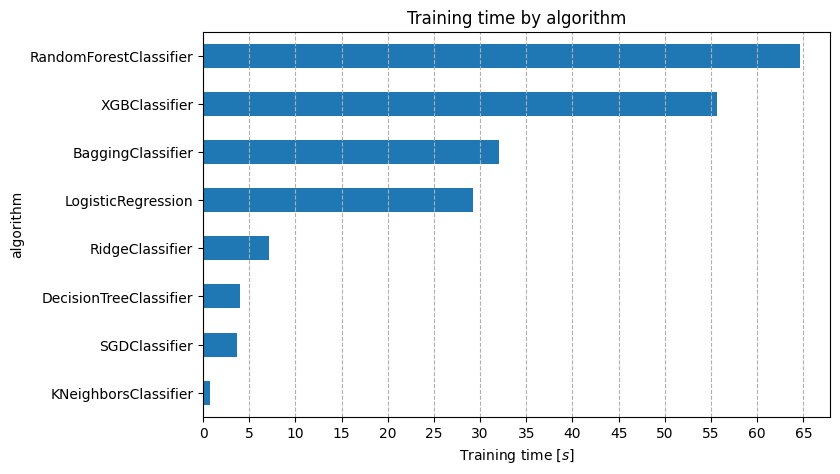
\includegraphics[width=0.9\textwidth]{training_time_uet.png}
				\caption{Tiempo de entrenamiento por algoritmo.}
				\label{fig:training_time_uet}
			\end{center}
		\end{figure}
						
		\textbf{Tiempo de inferencia}
						
		En la mayoría de algoritmos el tiempo de inferencia no supera los $20ms$, siendo la media de $5ms$. \texttt{KNC} y \texttt{RFC} muestran una gran cantidad de \textit{outliers} y tiempos superiores a la media.
						
		\begin{figure}[H]
			\begin{center}
				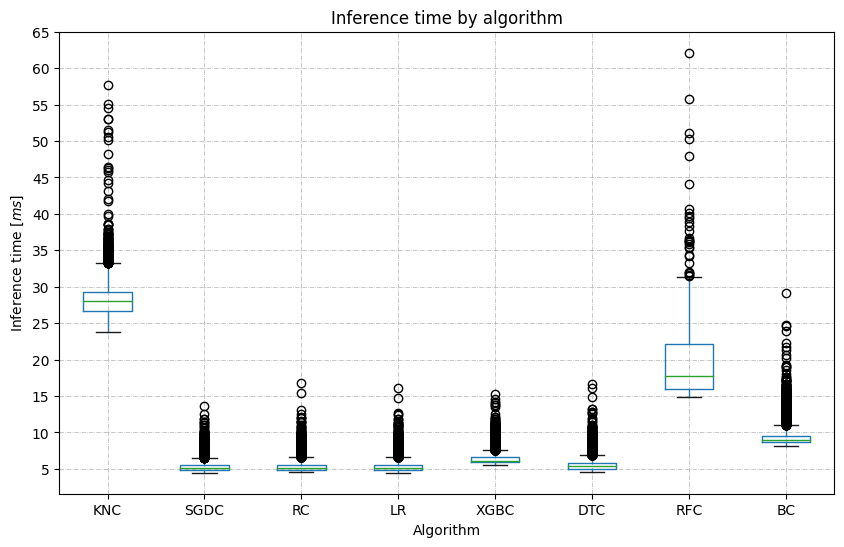
\includegraphics[width=0.9\textwidth]{inference_time_uet.png}
				\caption{Tiempo de inferencia por algoritmo.}
				\label{fig:inference_time_uet}
			\end{center}
		\end{figure}
						
		\textbf{Comparación visual de métricas}
						
		El gráfico de dispersión presentado en la fig.~\ref{fig:inference_training_perfo_uet} nos permite visualizar que hay dos algoritmos candidatos: \texttt{LR} y \texttt{DTC}. \texttt{LR} exhibe tiempos de inferencia menores y mayor rendimiento, pero un tiempo de entrenamiento superior a \texttt{DTC}. Actualmente el tiempo de entrenamiento es el criterio de menor importancia, por consiguiente \texttt{LR} será el algoritmo para imputar los datos faltantes de \texttt{TIPO}.
						
		\begin{figure}[H]
			\begin{center}
				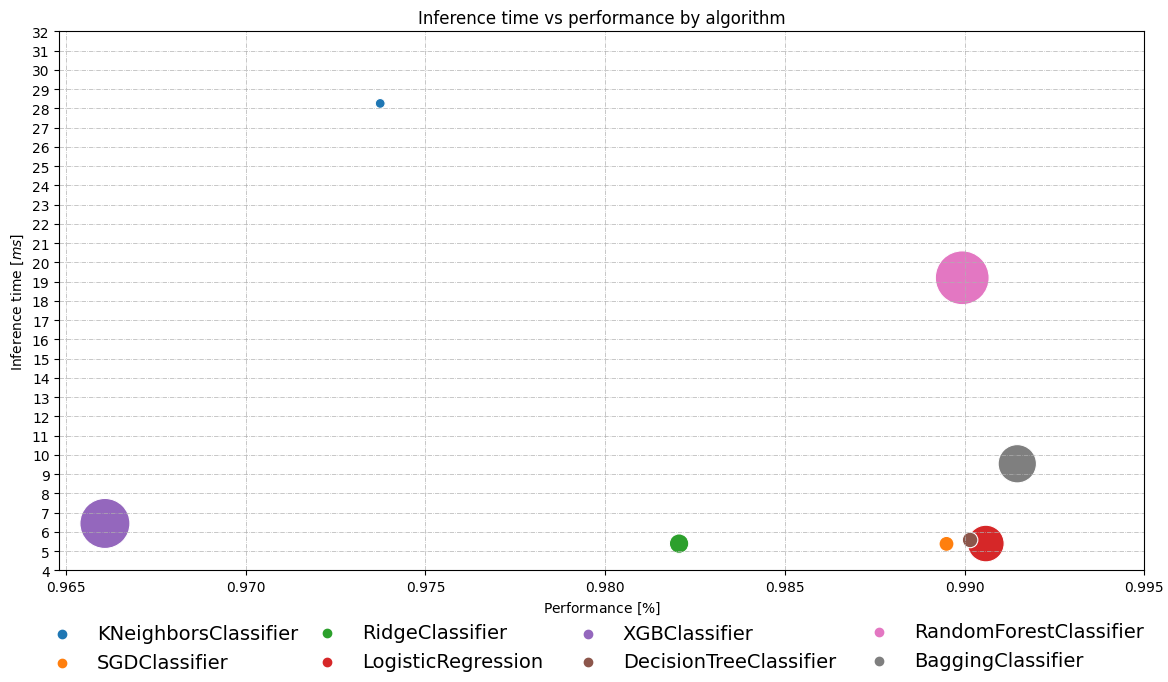
\includegraphics[width=1\textwidth]{inference_training_perfo_uet.png}
				\caption{Gráfico de dispersión de métricas por algoritmo.}
				\label{fig:inference_training_perfo_uet}
			\end{center}
		\end{figure}
						
		Para finalizar añadiremos que la fábrica posee personal y procesos específicos para determinar el origen de un defecto (\texttt{UET}) y de a que familia pertenece (\texttt{TIPO}). Implementando algunos de estos algoritmos se podría aliviar su carga de trabajo o  reasignar sus horas laborales a tareas de mayor impacto.
						
		\subsubsection{\href{https://github.com/GeraCollante/tesis-icomp-machinelearning/blob/main/DataFormatting.ipynb}{\color{blue}Formateo de datos}}\label{DataFormatting}
						
		El paso final antes de alimentar nuestro modelos es obtener rodajas (\textit{slices}) de tiempo con funciones de agregación de tipo \texttt{sum}, \texttt{count}, entre otras de nuestros datos. 
						
		\clearpage				
						
		\textbf{Serie temporal univariada}
						
		Pero como observamos en la Fig.~\ref{fig:graf_cantdef_antes}, nuestra serie temporal dista mucho de ser continua. Esto es un inconveniente ya que se ha demostrado que a los modelos les cuesta mucho aprender sobre series temporales intermitentes.
						
		Por esta razón se tomarán las siguientes consideraciones:
						
		\begin{itemize}[noitemsep, topsep=2pt]
			\item tomar el periodo posterior a la cuarentena por \textit{Sars-CoV-2}.
			\item quitar los días sin o con baja producción.
			\item quitar horarios no laborales.
		\end{itemize}
						
		En la Fig.~\ref{fig:graf_inter_antes} donde aplicamos la función escalón, notamos los huecos que tenemos en nuestra serie, por ello se aplicarán diversas funciones sobre la misma para obtener la serie continua deseada.
				
		\begin{figure}[]
			\begin{center}
				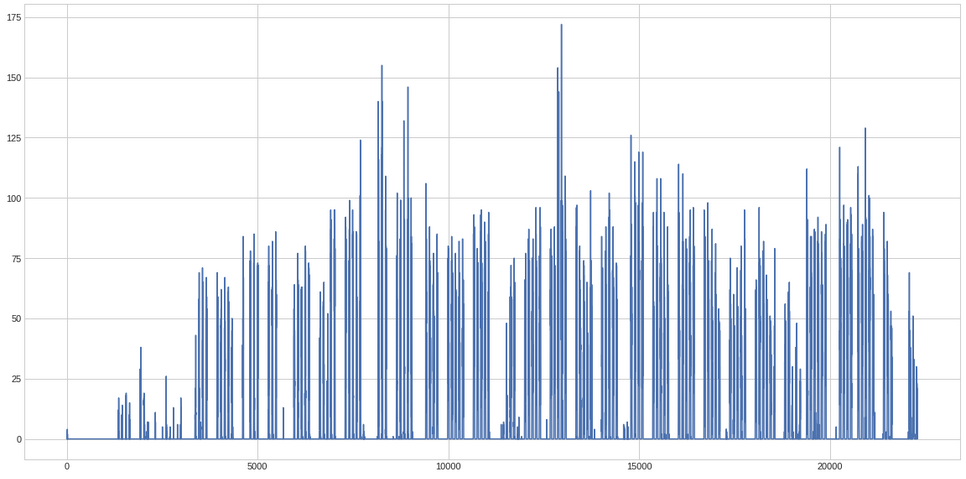
\includegraphics[width=1\textwidth]{tesis_78.png}
				\caption{Gráfico temporal de cantidad de defectos.}
				\label{fig:graf_cantdef_antes}
			\end{center}
		\end{figure}
						
		\begin{figure}[]
			\begin{center}
				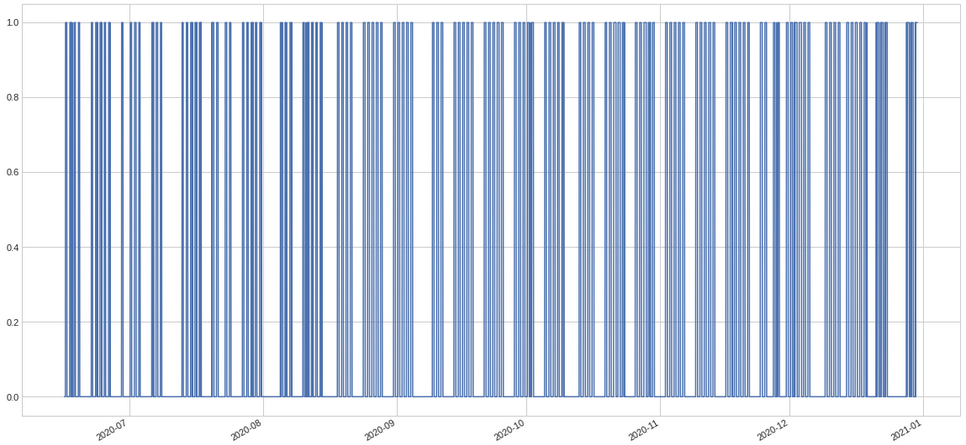
\includegraphics[width=1\textwidth]{tesis_79.png}
				\caption{Gráfico temporal de detección de intermitencia.}
				\label{fig:graf_inter_antes}
			\end{center}
		\end{figure}
						
		Una vez aplicado los filtros necesarios obtenemos la siguiente serie de la Fig.~\ref{fig:graf_cantdef_desp}. 
				
		En la Fig.~\ref{fig:graf_inter_desp} si bien siguen apareciendo ceros, aparecen en menor cantidad siendo originados en horarios de producción mínima como el horario de inicio y finalización.
						
		\begin{figure}[]
			\begin{center}
				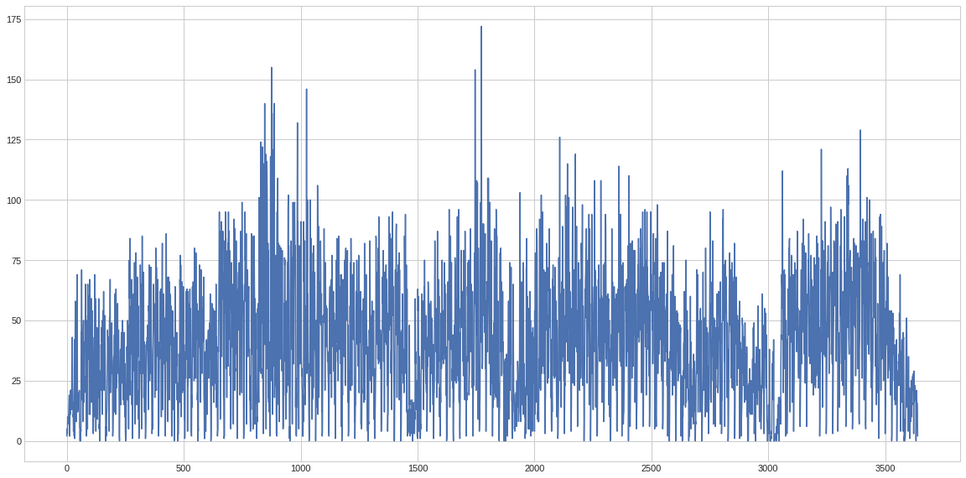
\includegraphics[width=1\textwidth]{tesis_80.png}
				\caption{Gráfico temporal de cantidad de defectos procesado.}
				\label{fig:graf_cantdef_desp}
			\end{center}
		\end{figure}
						
		\begin{figure}[]
			\begin{center}
				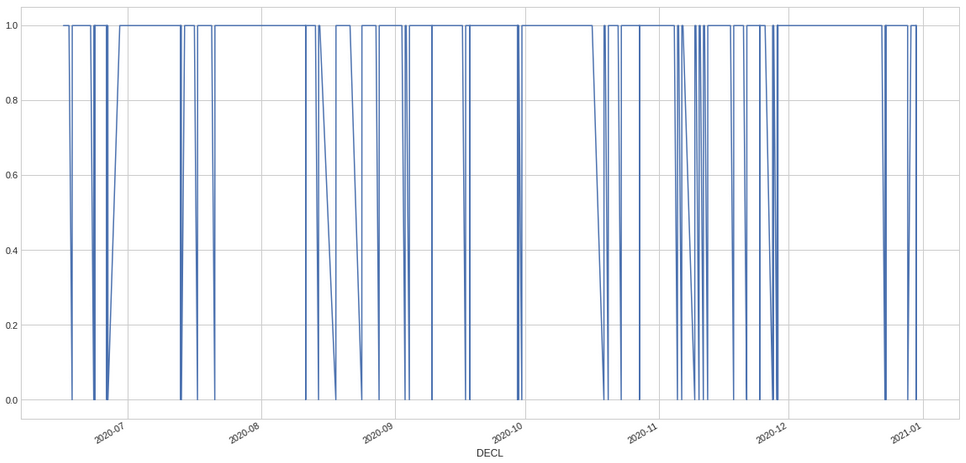
\includegraphics[width=1\textwidth]{tesis_81.png}
				\caption{Gráfico temporal de detección de intermitencia  procesado.}
				\label{fig:graf_inter_desp}
			\end{center}
		\end{figure}
						
		\textbf{Serie temporal multivariada}
						
		El mismo análisis realizado para la serie univariada debe extrapolarse a la cantidad de dimensiones que consideremos necesarias. 
						
		En la fig.~\ref{fig:graf_mult_dpto} observamos la cantidad de defectos que luego son desglosados por departamento, lo que nos daría 8 \textit{features}. 
				
		En la fig.~\ref{fig:graf_mult_tipo} los defectos son desglosados por tipo, lo que nos daría 11 \textit{features}. Lo que resultaría en 19 \textit{features} que van a alimentar nuestro modelo.
						
		\begin{figure}[H]
			\begin{center}
				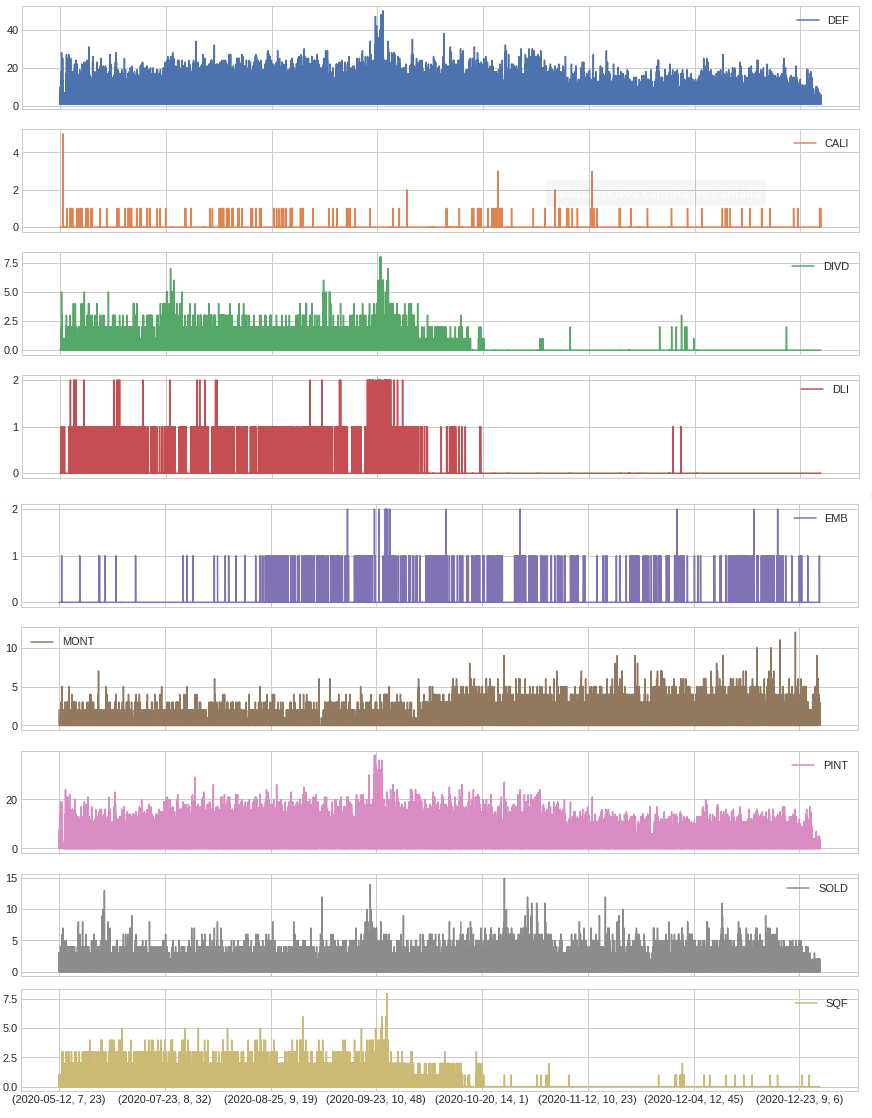
\includegraphics[width=1\textwidth]{multi_dpto.png}
				\caption{Gráfico temporal por departamentos.}
				\label{fig:graf_mult_dpto}
			\end{center}
		\end{figure}
						
		\begin{figure}[H]
			\begin{center}
				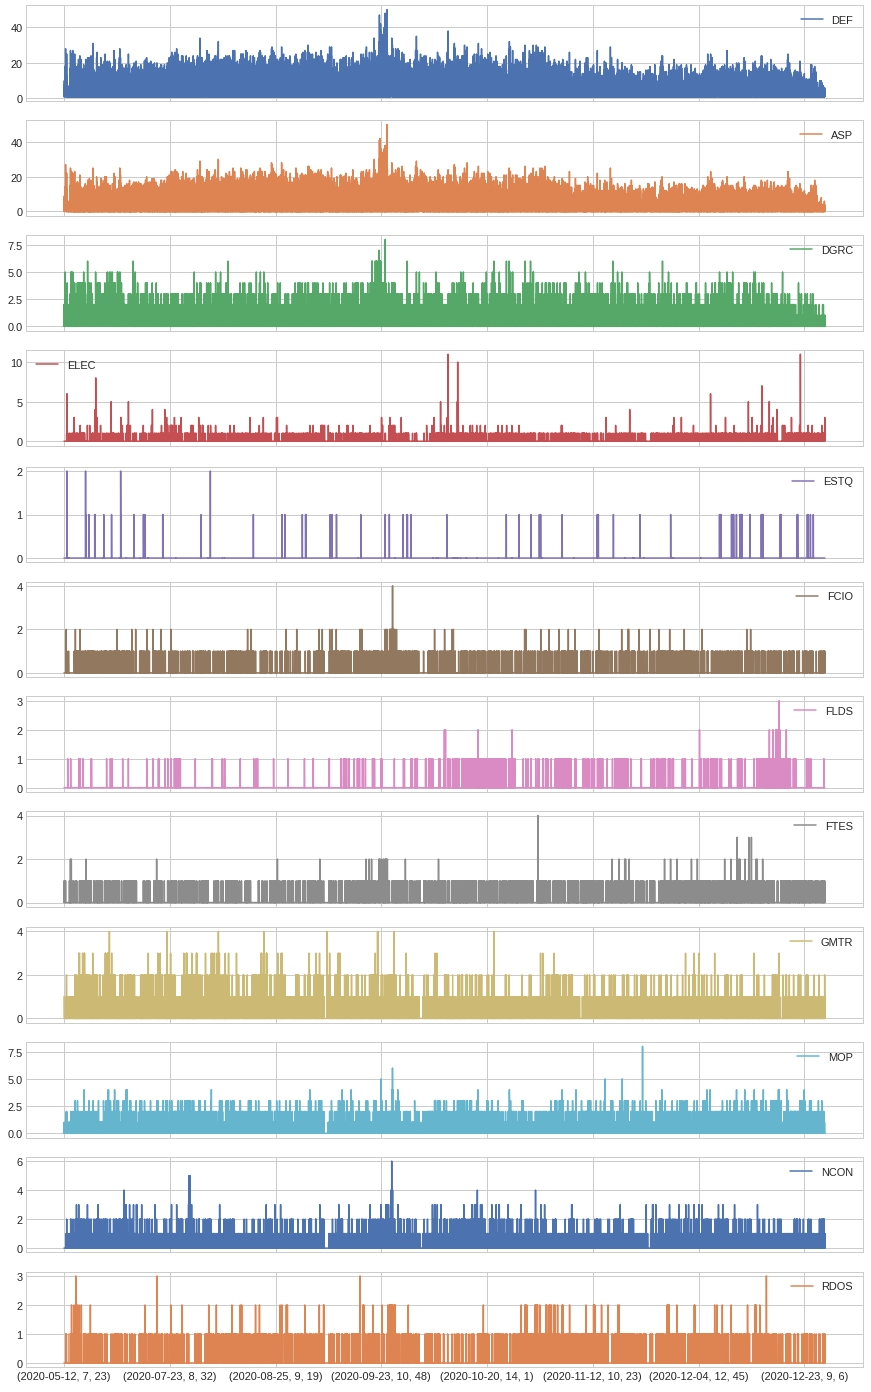
\includegraphics[width=0.93\textwidth]{multi_flia.png}
				\caption{Gráfico temporal por tipo de defecto.}
				\label{fig:graf_mult_tipo}
			\end{center}
		\end{figure}
						
		Tal como se realizó en la serie temporal univariada, se aplican los mismos pasos a estas series temporales de lo cual resultan las figuras \ref{fig:graf_post_mult_dpto} y \ref{fig:graf_post_mult_tipo}.
						
		\begin{figure}[H]
			\begin{center}
				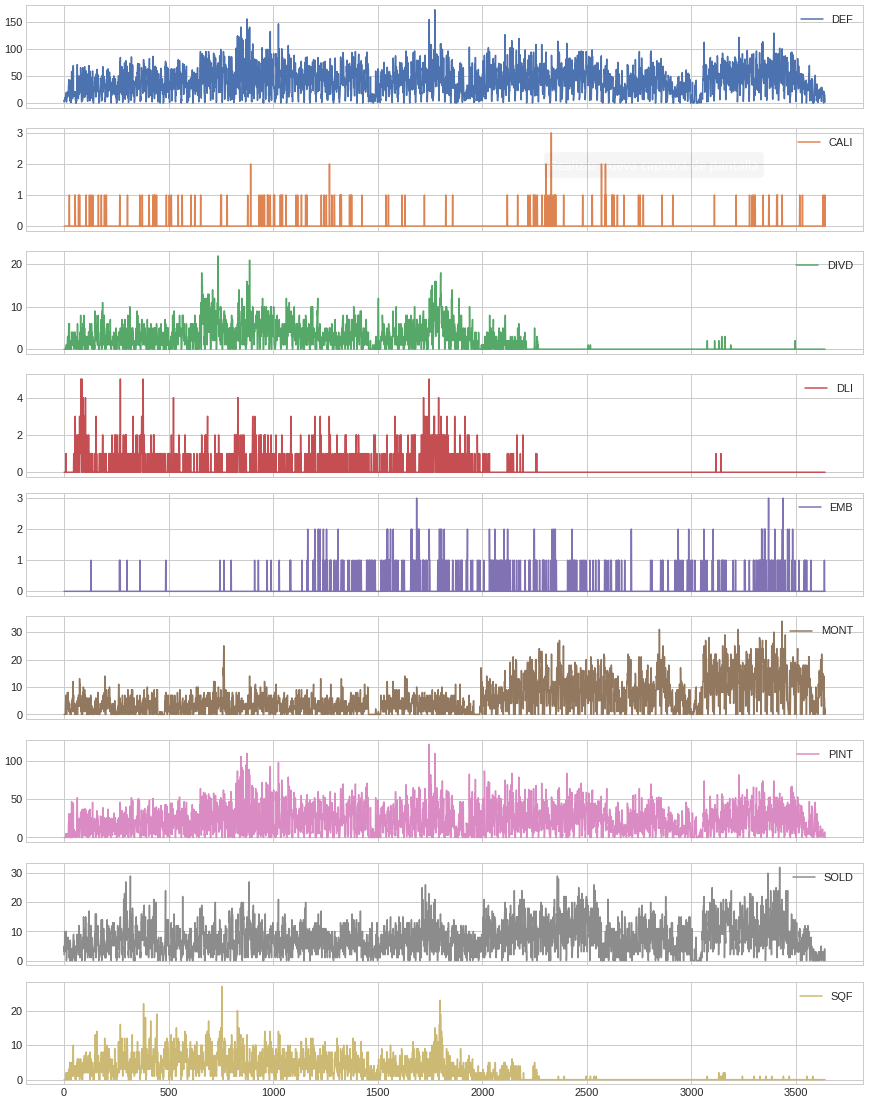
\includegraphics[width=1\textwidth]{multi_post_dpto.png}
				\caption{Gráfico temporal procesado por departamentos.}
				\label{fig:graf_post_mult_dpto}
			\end{center}
		\end{figure}
						
		\begin{figure}[H]
			\begin{center}
				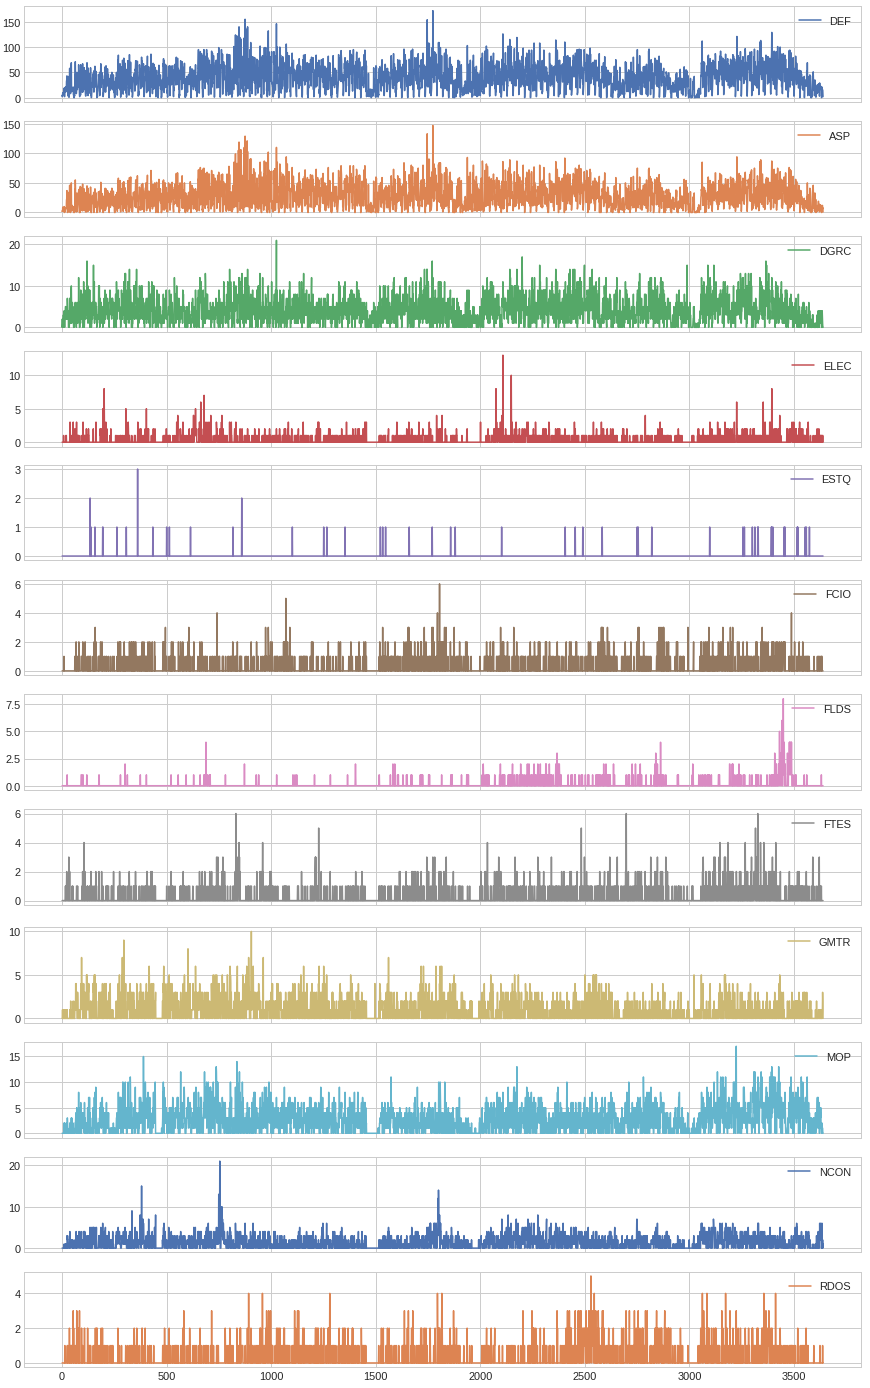
\includegraphics[width=0.93\textwidth]{multi_post_flia.png}
				\caption{Gráfico temporal procesado por tipo de defecto.}
				\label{fig:graf_post_mult_tipo}
			\end{center}
		\end{figure}
						
		Ya tenemos los \textit{datasets} definitivos formateados de una manera correcta para alimentar nuestros modelos.
						
		\subsubsection{\textit{Pipeline} de datos}
		Detengámonos a pensar sobre el tipo de problema con el que estamos tratando en el eventual caso que contáramos con los recursos para crear la arquitectura necesaria.
		En ingeniería de datos la arquitectura que orienta el flujo de datos se conoce como \textit{pipeline} de datos.
						
		El término \textit{pipeline} de datos puede describir cualquier conjunto de procesos que mueven datos de un sistema a otro, a veces transformando los datos, a veces no. Básicamente, se trata de una serie de pasos en los que se mueven los datos. Este proceso puede incluir medidas como duplicación de datos, filtrado, migración a la nube y procesos de enriquecimiento de datos. \citep{Tobin2020Jun}
						
		\textbf{Componentes}
						
		Las \textit{pipelines} de datos contienen varios componentes, cada uno con un propósito específico, que facilitan el movimiento de datos:
		\begin{itemize}[noitemsep, topsep=2pt]
			\item \textbf{Origen}: el origen representa la fuente de la que residen los datos originales.
			\item \textbf{Destino}: punto final al que se transfieren los datos, éste puede ser un almacén de datos (\textit{Data Warehouse}), un punto final de API, una herramienta de análisis o más.
			\item \textbf{Flujo de datos}: movimiento de datos entre el origen y el destino.
			\item \textbf{Sistema de almacenamiento}: se refiere a todos los sistemas utilizados para preservar los datos a lo largo de las etapas del flujo de datos.
			\item \textbf{Procesamiento}: incluye todas las actividades involucradas en el movimiento de los datos.
			\item \textbf{Flujo de trabajo}: representa una serie de procesos junto con sus dependencias para mover datos a través del \textit{pipeline}.
			\item \textbf{Monitoreo}: asegura que todas las etapas del \textit{pipeline} estén funcionando correctamente.
		\end{itemize}
						
		\textbf{\textit{Pipeline} ETL}
						
		Los ETL son flujos de trabajo automatizados que llevan los datos del punto A al punto B y los transforman a lo largo del camino para mejorar su capacidad de análisis o que se parezcan más a lo que nosotros necesitamos. ETL se refiere a extraer (\textit{Extract}), transformar (\textit{Transform}) y cargar (\textit{Load}) datos. \citep{SeattleDataGuy}
						
		En la fase de \textbf{extracción}, los datos a menudo se limitan a ser una instantánea de la base de datos en el momento actual o todos los datos históricos. Cuando extrae sus datos de la base de datos de una aplicación, a menudo los coloca en algún tipo de extracto \texttt{CSV} o \texttt{JSON}. 
				
		Estos extractos pueden provenir de tablas de bases de datos, APIs, registros, etc. Una vez que los datos se \textbf{transforman}, se \textbf{cargan} en el almacén de datos (\textit{Data Warehouse}).
						
		\textbf{\textit{Pipelines} de datos \textit{vs} \textit{pipelines} ETL}
						
		La diferencia entre estos dos estructuras de flujo de datos radica principalmente en que un \textit{pipeline} de datos es un término general del cual los \textit{pipelines} ETL son un subconjunto. \citep{Tobin2020Jun}
						
		\begin{table}[H]
			\centering
			\begin{tabular}{p{0.22\linewidth}|p{0.32\linewidth}|p{0.32\linewidth}}
				\hline
				\textbf{Característica} & \textbf{\textit{Pipeline} de datos} & \textbf{\textit{Pipelines} ETL} \\ \hline
				Carga de datos &
				No ocurre siempre. Si ocurre puede desencadenar nuevos procesos y flujos en otros sistemas. &
				Siempre termina en una base de datos o almacén de datos. \\
				Transformación          & No necesariamente.                  & Siempre.                        \\
				Modo de trabajo &
				Tiempo real. Los datos están actualizándose constantemente. &
				En lotes. Usualmente se corre unas dos veces por día, generalmente cuando el tráfico es bajo. \\ \hline
			\end{tabular}
			\caption{Diferencias entre pipelines de datos y ETL.}
			\label{tab:pipelines-table}
		\end{table}
						
		\textbf{\textit{DAG}}
						
		Usar la metáfora del \textit{pipeline}, ayuda a explicar un proceso que de otro modo sería complejo. Pero los datos no están literalmente en un solo \textit{pipeline}, comenzando por un lado y saliendo por el otro, pero esto nos sirve para destacar algunas características: \citep{astronomer}
		\begin{itemize}[noitemsep, topsep=2pt]
			\item Cuando los datos se mueven a través de pipelines, se aíslan de otros datos.
			\item Los datos deben tratarse en varias etapas antes de que lleguen a su destino.
		\end{itemize}
						
		Pero esto lleva a una linealidad en el flujo de datos que podría hacer que una estructura no pueda ser dinámica. Una solución a esta problemática son los \textit{DAG}s (\textit{Directed Acyclic Graphs)}, grafos acíclicos dirigidos.
						
		Clarifiquemos el concepto a través de la fig.~\ref{fig:dag} que expone el caso de una multinacional que recibe pagos en diferentes países, dónde en cada uno los clientes pagan en su moneda local. Para crear los reportes es necesario unificar las ventas de cada país teniendo en cuenta las diversas divisas.
						
		\begin{figure}[H]
			\begin{center}				
				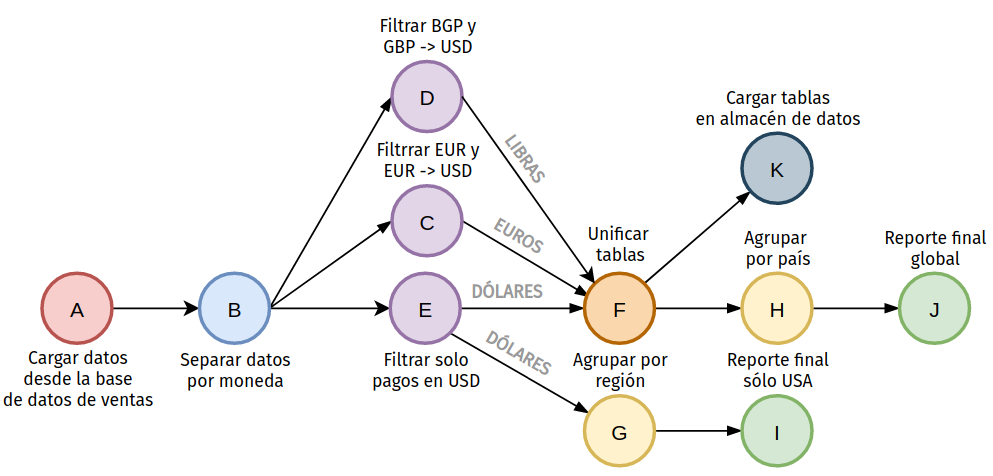
\includegraphics[width=1\textwidth]{dag.png}
				\caption{Ejemplo de grafo acíclico dirigido aplicado a caso real.}
				\label{fig:dag}
			\end{center}
		\end{figure}
						
		En matemáticas, un grafo es un conjunto finito de nodos, con vértices que conectan los nodos entre sí. En el contexto de la ingeniería de datos, cada nodo de un gráfico representa una tarea de procesamiento de datos y cada vértice (línea) tiene una dirección específica (indicada por la flecha) que conecta diferentes nodos. Ésta es la cualidad clave de un grafo dirigido: los datos solo pueden seguir la dirección del vértice. Además tener en cuenta que los nodos nunca se vuelven autorreferenciales, \textit{i.e.} nunca pueden informarse a sí mismos, ya que esto podría crear un bucle infinito.
						
		Resumiendo un \textit{DAG} se caracteriza por ser:
		\begin{itemize}[noitemsep, topsep=2pt]
			\item \textbf{Grafo}: todas las tareas se presentan en una estructura clara, con procesos discretos que ocurren en puntos establecidos y relaciones transparentes con otras tareas.
			\item \textbf{Acíclico}: ninguna tarea puede crear datos que se refieran a sí misma. Podría causar un bucle infinito y eso podría causar problemas.
			\item \textbf{Dirigido}: si existen varias tareas, cada una debe tener al menos una tarea definida en sentido ascendente o descendente, aunque podría tener ambas.
		\end{itemize}
						
		\textbf{Categorización del problema}
						
		Observemos la figura \ref{fig:dag_fsi} para ponernos en contexto. Esta figura es un \textit{DAG} del flujo de datos de nuestro sistema, dónde cada nodo es representado por las notebooks que se detallaron con anterioridad.
						
		\begin{figure}[H]
			\begin{center}
				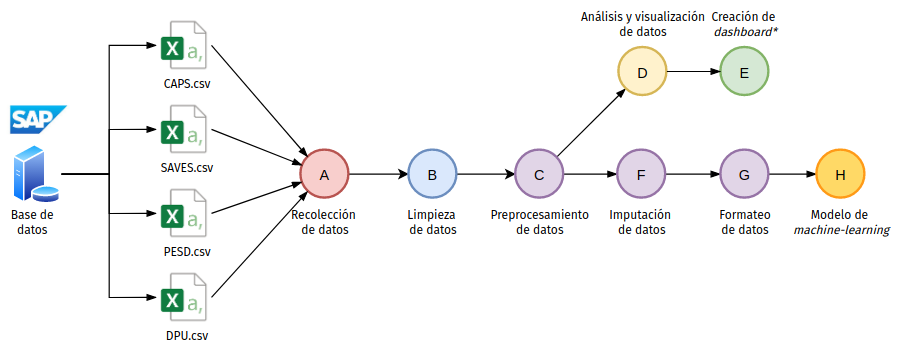
\includegraphics[width=1\textwidth]{dag_fsi.png}
				\caption{\textit{DAG} del flujo de datos.}
				\label{fig:dag_fsi}
			\end{center}
		\end{figure}
						
		En primera instancia los datos son obtenidos (nodo A, fase de extracción) desde archivos \texttt{.csv} debido a que por políticas de la compañía, los datos se guardan en bases de datos de \texttt{SAP} y los empleados del departamento realizan extracciones diarias de forma manual para actualizar estos archivos. No es posible realizar consultas \texttt{SQL} o llamadas a una API (por nombrar algunos métodos de extracción de datos), por lo cuál este proceso no se puede automatizar.
						
		Esto deviene en un impedimento crítico hacía nuestro sistema ya que por la naturaleza del problema a tratar (series temporales) es indispensable que el flujo de datos al modelo sea constante y en tiempo real (\textit{streaming} de datos).
						
		Los nodos B, C, F y G corresponderían a la etapa de transformación, no obstante estos datos no son almacenados por tanto nuestro flujo de datos no encuadra en un \textit{pipeline} ETL.
						
		Los nodos D y E* (esta notebook no fue creada debido a que no se solicitó) corresponden a las etapas de análisis y visualización. Un punto a destacar es que esta etapa sería de gran valor para la compañía ya que permite visualizar datos de un modo que antes no era posible (recordar que los datos debieron pasar por los nodos B y C para llegar a esta instancia), lo que lleva a una reducción de costes debido a mayor reactividad en la detección de defectos.
						
		En última instancia está el modelo, que recibe los datos en un formato acorde, se encarga de procesarlos y realiza la inferencia. Quitando los nodos D y E, nuestro problema se ajusta a la categoría de \textit{pipeline} de datos.
						
		\clearpage
						
		\section{Modelos}\label{TrainingModel}
						
		Los modelos serán creados combinando las diferentes capas que se han definido con anterioridad.
						
		\subsection{Métricas}
						
		Es importante definir métricas para determinar el rendimiento de nuestro modelo de una manera empírica, más allá de que nuestros modelos serán entrenados utilizando como métrica de pérdida \texttt{MAE} (error absoluto medio).
						
		\subsubsection{\texttt{MAPE}}
						
		Una de las métricas más habituales para medir la precisión del pronóstico de un modelo es \texttt{MAPE}, que significa error porcentual absoluto medio (\textit{mean absolute percentage error}). \citep{MAPE}
						
		La fórmula para calcular \texttt{MAPE} es la siguiente:
						
		$$ \texttt{MAPE} = \frac{100}{N} \times \sum_{i=1}^{N} |\frac{y_i - \hat{y_i}}{y_i}| $$
						
		dónde:
						
		\begin{itemize}[noitemsep, topsep=2pt]
			\item $ y_i$: valores de los datos reales.
			\item $ \hat{y_i}$: valor de datos pronosticados.
			\item $ N $: cantidad de puntos.
		\end{itemize}
						
		\texttt{MAPE} se usa generalmente debido a su fácil interpretación y simple explicación. Por ejemplo, un valor \texttt{MAPE} de $11,5\%$ significa que la diferencia promedio entre el valor pronosticado y el valor real es $11,5\%$. Cuanto menor sea el valor de \texttt{MAPE}, mejor podrá un modelo pronosticar valores.
						
		Sin embargo esta métrica no nos será de utilidad ya que si alguno de los valores reales es $0$ (como sucede) entonces el valor será incalculable por la división por $0$. 
						
						
						
		\subsubsection{\texttt{MASE}}
		En el pronóstico de series temporales, el \texttt{MASE} es el error medio absoluto escalado (\textit{Mean Absolute Scaled Error}). Es una métrica para determinar la efectividad de los pronósticos generados a través de un algoritmo al comparar las predicciones con el resultado de un enfoque de pronóstico ingenuo o \textit{naive forecast}. \citep{MASE}
						
		El \textit{naive forecast} se genera en cualquier paso equiparando el pronóstico actual con la salida del último paso de tiempo. Por ejemplo, la predicción de las ventas de una empresa al comienzo de un mes se realiza comparándola con las ventas reales del último mes sin considerar ningún patrón estacional.
						
		El \texttt{MAE} para \textit{naive forecast} se calcula de la siguiente forma:
						
		$$
		\texttt{MAE}_{naive} = \frac{1}{N-1} \sum_{i=2}^N |y_i - y_{i-1}|
		$$
						
		Para determinar la efectividad de un algoritmo de pronóstico, el \texttt{MASE} se calcula de la siguiente manera:
						
		\begin{enumerate}[noitemsep, topsep=2pt]
			\item Calcular el \texttt{MAE} (\textit{Mean Absolute Error}) para los prónosticos del algoritmo.
			      			      			      	
			      $$
			      \texttt{MAE} = \frac{1}{N} \sum_{i=1}^N |\hat{y_i} - y_i|	
			      $$	
			\item \texttt{MASE} está dado por el ratio entre el \texttt{MAE} del algoritmo y el \texttt{MAE} del \textit{naive forecast}.
			      			      			      	
			      $$
			      \texttt{MASE} = \frac{\texttt{MAE}}{\texttt{MAE}_{naive}}	
			      $$
			      			      			      	
		\end{enumerate}
						
		\textbf{Características}
		\begin{itemize}%[noitemsep, topsep=2pt]
			\item \texttt{MASE} da una indicación de la eficacia del algoritmo de pronóstico con respecto a un \textit{naive forecast}. Un valor mayor a uno indica que el algoritmo está funcionando mal en comparación al \textit{naive forecast}.
			      			      			      
			\item \texttt{MASE} es inmune al problema que enfrenta \texttt{MAPE} cuando la salida de la serie de tiempo real en cualquier paso de tiempo es cero. Sin embargo, se observa que para una serie de tiempo con todos los valores iguales a cero en todos los pasos, la salida de \texttt{MASE} tampoco se definirá, pero tales series de tiempo no son realistas.
			      			      			      	
			      			      			      		
			      			      			      	
			\item \texttt{MASE} es independiente de la escala del pronóstico, ya que se define utilizando la proporción de errores. Esto significa que los valores de \texttt{MASE} serán similares si pronosticamos series de tiempo de alto valor, como el número de paquetes de tráfico de Internet que cruzan un router por hora, en comparación con el número de peatones que cruzan un semáforo ocupado cada hora.
		\end{itemize}
						
		\subsection{\textit{Framework}}
						
		Al momento de definir el \textit{framework} de \textit{Machine Learning} podemos encontrar 2 alternativas que se disputan el mayor porcentaje del mercado:
		\begin{itemize}[noitemsep, topsep=2pt]
			\item \textit{TensorFlow}: es una biblioteca de código abierto para aprendizaje automático a través de un rango de tareas, y desarrollado por \textit{Google} para satisfacer sus necesidades de sistemas capaces de construir y entrenar redes neuronales para detectar y descifrar patrones y correlaciones, análogos al aprendizaje y razonamiento usados por los humanos. Usualmente se utiliza como \textit{back-end} de otro \textit{framework} llamado \textit{Keras} que posee una API más amigable con el usuario.
			\item \textit{PyTorch}: es una biblioteca de aprendizaje automático​ de código abierto basada en la biblioteca de \textit{Torch}, utilizado para aplicaciones del campo de la visión artificial y del procesamiento natural del lenguaje, principalmente desarrollado por el Laboratorio de Investigación de Inteligencia Artificial​ de \textit{Facebook}.
		\end{itemize}
						
		Los datos recopilados por la página \textit{PapersWithCode} \citep{trendsML} en la fig.~\ref{fig:fw_market} nos muestra una clara tendencia de los investigadores a preferir \textit{PyTorch} sobre los demás \textit{frameworks}.
						
		\begin{figure}[H]
			\begin{center}
				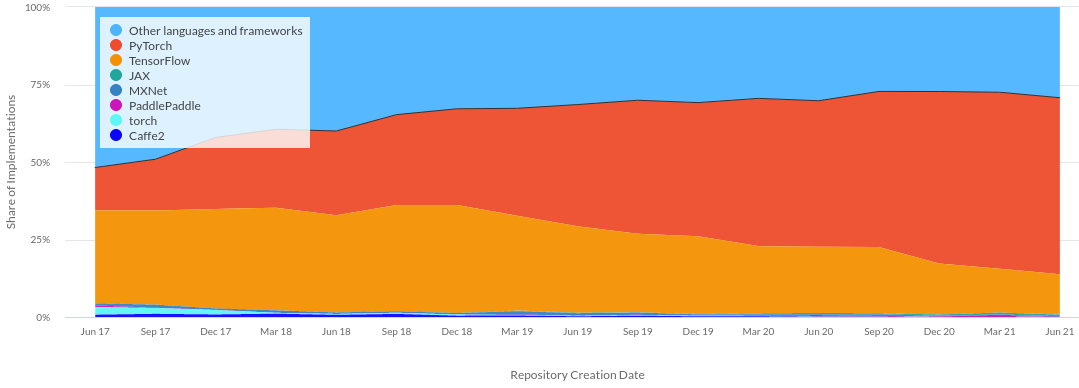
\includegraphics[width=1\textwidth]{fw_market.png}
				\caption{Porcentaje de implementaciones de cada \textit{framework} en \textit{papers}.}
				\label{fig:fw_market}
			\end{center}
		\end{figure}
						
		A pesar de esto para nuestra tarea debido a su facilidad de uso se escogió \textit{Keras}, biblioteca de redes neuronales de código abierto cuyo autor principal es el ingeniero François Chollet.
						
		Está especialmente diseñada para posibilitar la experimentación en un corto plazo con redes de Aprendizaje Profundo. Sus fuertes se centran en ser amigable para el usuario, modular y extensible. \citep{keras-wiki}
						
		\subsubsection{Callbacks}
		Una característica muy interesante que nos ofrece \textit{Keras} son las \textit{callbacks}. Se define como un objeto que puede realizar acciones en varias etapas del entrenamiento (por ejemplo, al comienzo o al final de una época, antes o después de un solo lote, etc.). Repasaremos algunas de las que fueron utilizadas en el entrenamiento del modelo. \citep{callbacks}
						
		\begin{itemize}[noitemsep, topsep=2pt]
			\item \texttt{EarlyStopping}: detiene el entrenamiento cuando una métrica monitoreada haya dejado de mejorar. Asumimos que el objetivo de un entrenamiento es minimizar la pérdida, \textit{e.g.} la métrica a monitorear sería \texttt{loss} y el modo sería \texttt{min}. Un ciclo de entrenamiento verificará al final de cada época si la pérdida ya no está disminuyendo, considerando el \texttt{min\_delta} y la paciencia (cantidad de épocas sin mejorar). Una vez que la métrica no disminuye, el entrenamiento termina. Esto es ventajoso para ahorrar tiempo de entrenamiento.
			\item \texttt{ReduceLROnPlateau} \label{plateau}: reduce la tasa de aprendizaje cuando una métrica ha dejado de mejorar. Los modelos usualmente se benefician de la reducción de la tasa de aprendizaje en un factor de 2 a 10 una vez que el aprendizaje se estanca. Esta \textit{callback} monitorea una métrica y si no se ve ninguna mejora en un número de épocas de "paciencia", la tasa de aprendizaje se reduce. Ha brindado excelentes resultados.
			\item \texttt{ModelCheckpoint}: trabaja en conjunto con el entrenamiento para guardar un modelo o pesos (en un archivo de punto de control) en algún intervalo, por lo que el modelo o los pesos se pueden cargar más tarde para continuar el entrenamiento desde el estado guardado.
			      Algunas opciones que ofrece:
			      \begin{itemize}[noitemsep, topsep=2pt]
			      	\item Mantener solo el modelo que ha logrado el "mejor desempeño" hasta ahora, o guardar el modelo al final de cada época sin importar el desempeño.
			      	\item La frecuencia a la que debería guardar. Actualmente, se permite guardar al final de cada época o después de un número fijo de lotes de entrenamiento.
			      	\item Si solo se guardan los pesos o se guarda todo el modelo.
			      \end{itemize}
		\end{itemize}
						
		\subsection{Arquitecturas} \label{archs}
		Se define como la arquitectura del modelo a la disposición del mismo en lo que concierne a sus capas y al flujo de la información a través de las mismas.
						
		\clearpage				
						
		En \textit{Keras} es posible definir un modelo \texttt{Sequential}, lo que significa que cada salida alimentará a la siguiente y no habrá bifurcaciones entre el flujo de los tensores. También se podría resumir que \texttt{Sequential} agrupa una pila lineal de capas, lo que para nuestro propósito es suficiente. Esto se denomina arquitectura de tipo lineal. A modo informativo en \textit{TensorFlow} es posible crear arquitecturas no-lineales que admitan múltiples flujos de datos entre las diferentes capas.
						
		\subsubsection{Hiperpárametros de capas}
		En la figura~\ref{fig:layer_types} podemos observar las capas disponibles para crear nuestra arquitectura.
						
		\begin{figure}[H]
			\begin{center}
				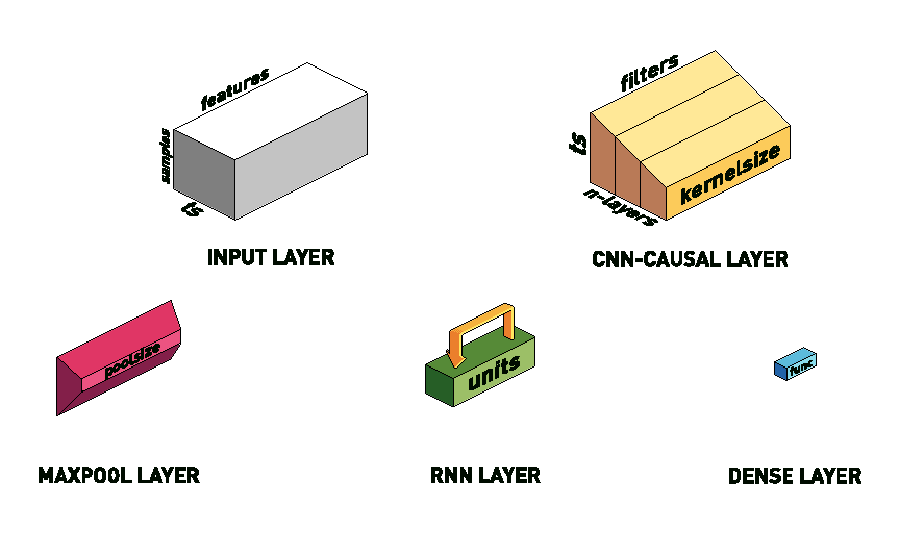
\includegraphics{model_types.eps}
				\caption{Tipos de capas disponibles.}
				\label{fig:layer_types}
			\end{center}
		\end{figure}
						
						
						
		Detallaremos los hiperpárametros que será posible \textit{tunear} de cada capa.
						
		\begin{itemize}[noitemsep, topsep=2pt]
			\item \texttt{INPUT}:
			      \begin{itemize}[noitemsep, topsep=2pt]
			      	\item \texttt{ts}: \textit{timestamps}.
			      	\item \texttt{features}: características.
			      	\item \texttt{samples}: cantidad de muestras.
			      \end{itemize}
			\item \texttt{CNN-CAUSAL}
			      \begin{itemize}[noitemsep, topsep=2pt]
			      	\item \texttt{n-layers}: cantidad de capas, podemos escalar en la profundidad de \texttt{CNN}s.
			      	\item \texttt{filters}: filtros.
			      	\item \texttt{kernelsize}: tamaño del \textit{kernel}.
			      	\item \texttt{ts} = \textit{timestamps} o rodajas de tiempo.
			      \end{itemize}
			\item \texttt{GRU} y \texttt{LSTM}
			      \begin{itemize}[noitemsep, topsep=2pt]
			      	\item \texttt{units}: unidades de la celda.
			      \end{itemize}
			\item \texttt{MAXPOOL}:
			      \begin{itemize}[noitemsep, topsep=2pt]		
			      	\item \texttt{poolsize}: tamaño de \textit{pool}.
			      \end{itemize}
			\item \texttt{FC}
			      \begin{itemize}[noitemsep, topsep=2pt]
			      	\item \texttt{func}: función de activación.
			      \end{itemize}
		\end{itemize}
						
		\subsubsection{Tipos}
						
		En función a las capas explicadas en el marco teórico se ensayarán 5 arquitecturas de modelo representadas de forma visual en la fig.~\ref{fig:arch_types}, con el objetivo de identificar la de mejor desempeño utilizando como parámetro la métrica \texttt{MASE}.
						
		\begin{itemize}[noitemsep, topsep=2pt]
			\item CNN: \texttt{CNN -> FC}
			\item LSTM: \texttt{LSTM -> FC}
			\item GRU: \texttt{GRU -> FC}
			\item CNNLSTM: \texttt{CNN -> MAXPOOL -> LSTM -> FC}
			\item CNNGRU: \texttt{CNN -> MAXPOOL -> GRU -> FC}
		\end{itemize}
						
		En el caso de las últimas dos redes se utilizó la capa de \texttt{MAXPOOL} para evitar el cuello de la botella de los datos, corroborando que no se afectó el rendimiento del modelo y mejoraron los tiempos de entrenamiento.
						
		\begin{figure}[H]
			\begin{center}
				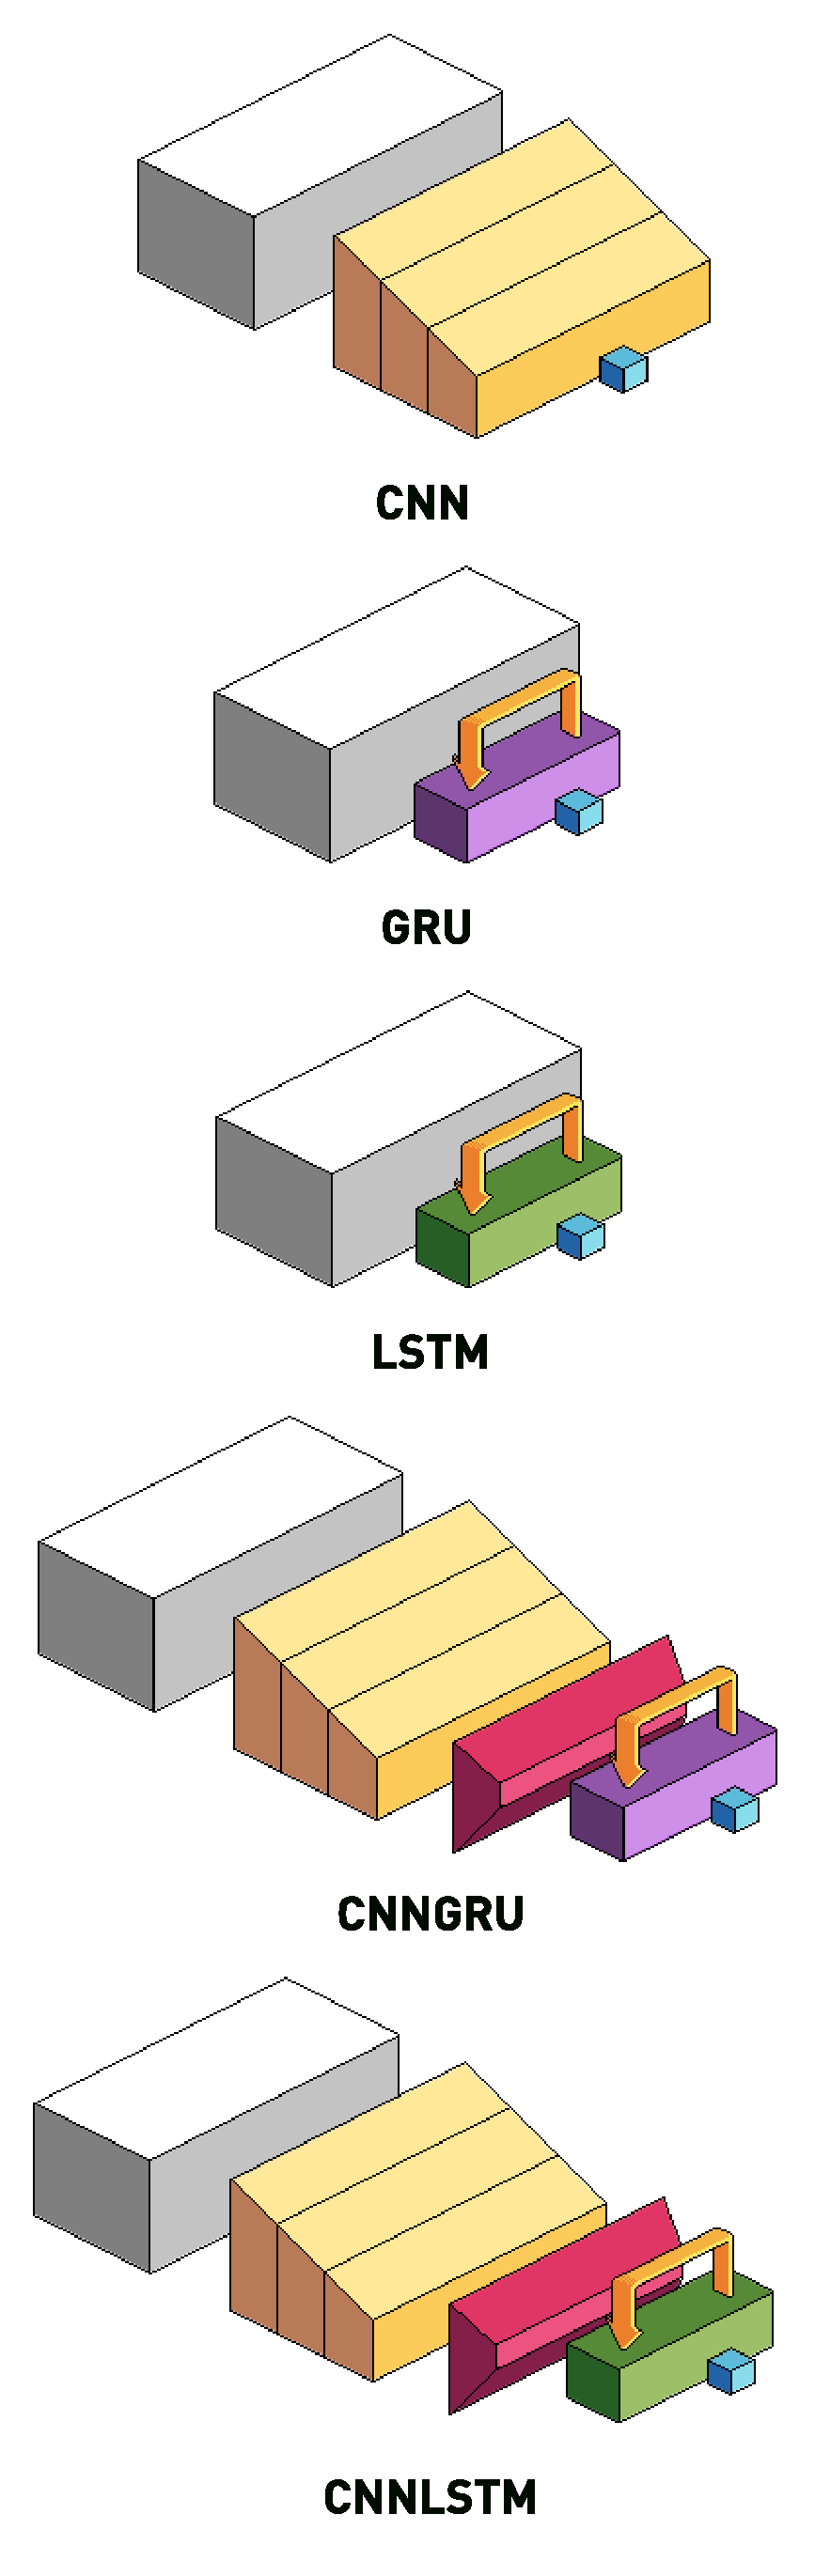
\includegraphics[width=0.45\textwidth]{layers.eps}
				\caption{Tipos de arquitecturas.}
				\label{fig:arch_types}
			\end{center}
		\end{figure}
						
		\subsection{\href{https://github.com/GeraCollante/tesis-icomp-machinelearning/blob/main/Models.ipynb}{\color{blue}Entrenamiento}}
						
		\subsubsection{Datos de prueba}
		Ya tenemos todos los ingredientes necesarios para empezar el entrenamiento de nuestra red neuronal, sin embargo sería coherente utilizar datos de prueba o \textit{dummy data} para corroborar que todo funcione según lo esperado.
						
		Para esta tarea haremos uso de un \textit{dataset} de los niveles de polución en el aire. Contiene detalles sobre diferentes parámetros que son monitoreados cada hora durante cinco años en la embajada de Estados Unidos en Beijing, China.
						
		Los datos incluyen la fecha y hora, la contaminación denominada concentración de PM2.5 y la información meteorológica. La lista completa de características en los datos es la siguiente:
						
		\begin{itemize}[noitemsep, topsep=2pt]
			\item \texttt{pollution}: concentración de PM2.5, son partículas muy pequeñas suspendidas en el aire que tienen un diámetro de menos de 2.5 micras. Será nuestro \textit{target}.
			\item \texttt{dew}: punto de rocío, es la más alta temperatura a la que empieza a condensarse el vapor de agua contenido en el aire, produciendo rocío, neblina, cualquier tipo de nube o, en caso de que la temperatura sea lo suficientemente baja, escarcha.
			\item \texttt{temp}: temperatura.
			\item \texttt{press}: presión.
			\item \texttt{wnd\_dir}: dirección del viento combinada.
			\item \texttt{wnd\_spd}: velocidad del viento acumulada.
			\item \texttt{snow}: horas acumuladas de nieve.
			\item \texttt{rain}: horas acumuladas de lluvia.
		\end{itemize}
						
		Bajo estos datos se enmarcará un problema de pronóstico en el que dadas las condiciones climáticas y la contaminación de las horas previas, pronosticamos la contaminación de la hora siguiente.
						
		En la fig.~\ref{fig:pollution_dataset} podemos observar que nuestros datos son bastante armoniosos notando 3 ondas sinusoidales, característica que el modelo explotará (pero la mayoría de las series temporales en la vida real no serán tan convenientes).
						 
		\begin{figure}[H]
			\begin{center}
				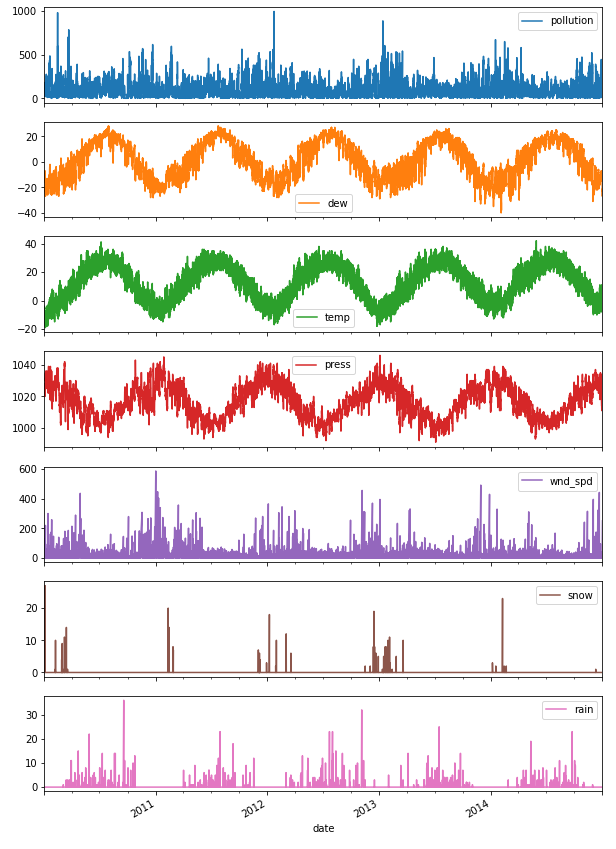
\includegraphics[width=1\textwidth]{pollution.png}
				\caption{\textit{Dataset} de contaminación del aire.}
				\label{fig:pollution_dataset}
			\end{center}
		\end{figure}
						
		Luego deberemos dividir nuestro \textit{dataset} como vimos con anterioridad en 3 sets en la siguiente proporción:
		\begin{itemize}[noitemsep, topsep=2pt]
			\item \texttt{train} (\textit{entrenamiento}): $70\%$.
			\item \texttt{validation} (\textit{validación}): $20\%$.
			\item \texttt{test} (\textit{prueba}): $10\%$.
		\end{itemize}
						
		Recordar que la métrica \texttt{val\_loss} será aplicada sobre el set de validación y \texttt{MASE} sobre el set de prueba.
						
		\begin{figure}[H]
			\begin{center}
				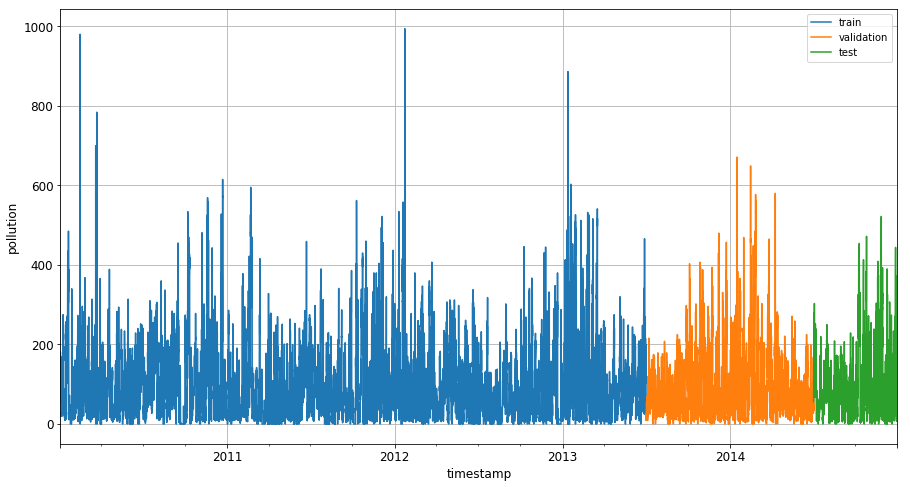
\includegraphics[width=0.9\textwidth]{tvt_pollution.png}
				\caption{\textit{Dataset} de contaminación del aire.}
				\label{fig:tvt_pollution}
			\end{center}
		\end{figure}
						
		\subsubsection{Desplazamiento temporal}
		Una operación importante a realizar en nuestro dataset es el desplazamiento temporal o \textit{time-shifting} para lograr que nuestra red pueda aprender sobre los \textit{timesteps} pasados de nuestras features y comparar su salida contra los \textit{timesteps} futuros en caso de ser la \textit{target feature}.
						
		Para aclarar esta idea pongamos nuestro enfoque en la figura \ref{fig:shift_explain}. Definiremos \texttt{T} a la cantidad de \textit{timesteps} que queremos que nuestro modelo utilice para extraer información pasada, además del actual.
						
		Y definiremos \texttt{HORIZON} como al horizonte de pronóstico, \textit{i.e.} la cantidad de \textit{timesteps} futuros que queremos predecir de nuestra característica objetivo o \textit{target feature}.
						
		\begin{figure}[H]
			\begin{center}
				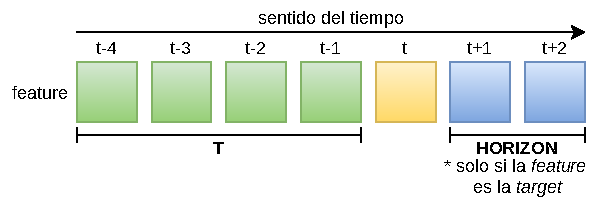
\includegraphics[width=0.55\textwidth]{time-shift.pdf}
				\caption{Desplazamiento temporal visualizado.}
				\label{fig:shift_explain}
			\end{center}
		\end{figure}
						
		\subsubsection{Tipo de horizonte}
		Un punto importante a aclarar es que es diferente la arquitectura a implementar según si nuestra \textit{target feature} es de horizonte único o multi-horizonte.
						
		\hfill
						
		\textbf{Horizonte único}
						
		Veremos en una perspectiva más amplia el funcionamiento de nuestro modelo para tomar noción de donde nos encontramos y para esta tarea nos será útil la fig.~\ref{fig:unihorizon_model} \citep{rnn_azure}. Básicamente tomamos los \texttt{T} \textit{timesteps} de nuestras \textit{features} para alimentar a la arquitectura (que fueron presentadas en la sección \ref{archs}), en este caso compuesta de celdas \texttt{RNN}, que luego la salida alimenta una neurona que determina el valor de \texttt{t+1}.
						
		\begin{figure}[H]
			\begin{center}
				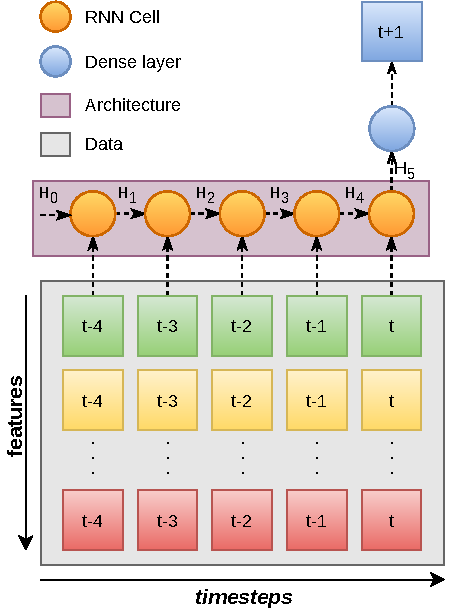
\includegraphics[width=0.46\textwidth]{unihorizon-model.pdf}
				\caption{Modelo de horizonte único.}
				\label{fig:unihorizon_model}
			\end{center}
		\end{figure}
						
		\textbf{Horizonte múltiple}
						
		Observemos la fig.~\ref{fig:multihorizon_model} \citep{rnn_ed_azure}. Si determinamos que nuestra \textit{target feature} será de horizonte múltiple, debemos aumentar la complejidad de nuestra arquitectura lo que se traduce en menor personalización en lo que se refiere a adición de capas.
						
		Debemos contar con dos capas \texttt{encoder} y \texttt{decoder}, donde una se encargará de procesar los datos de entrada y la otra de decodificar la salida de la primera para obtener la forma de tensor deseada a la salida de la red, lo que sería \texttt{t+1}, \texttt{t+2} y \texttt{t+3} en nuestro ejemplo.
						
		\begin{figure}[H]
			\begin{center}
				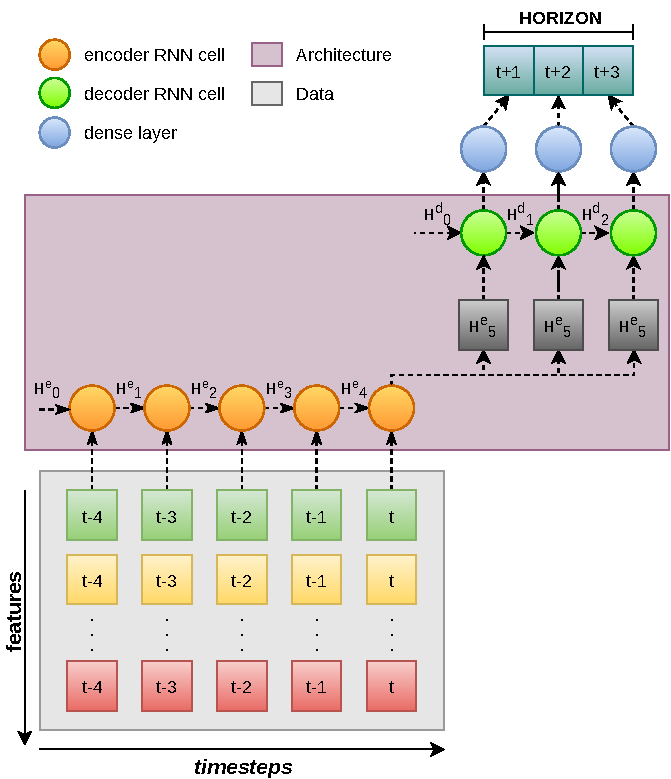
\includegraphics[width=0.9\textwidth]{multihorizon-model.pdf}
				\caption{Modelo de horizonte múltiple.}
				\label{fig:multihorizon_model}
			\end{center}
		\end{figure}
						
		En la fig.~\ref{fig:multihorizon_plot} podemos observar la salida de un pronóstico de horizonte múltiple con \texttt{T=16} y \texttt{HORIZON=4}. Notamos que a medida que queremos predecir pasos más lejanos perdemos precisión, en la tabla~\ref{tab:multi-horizon-results} se corrobora de manera numérica esta observación.
						
		Además cuando veamos los resultados de los modelos de horizonte único notaremos que \texttt{t+1} tiene mayor precisión que en este tipo de modelos.
						
		\begin{figure}[H]
			\begin{center}
				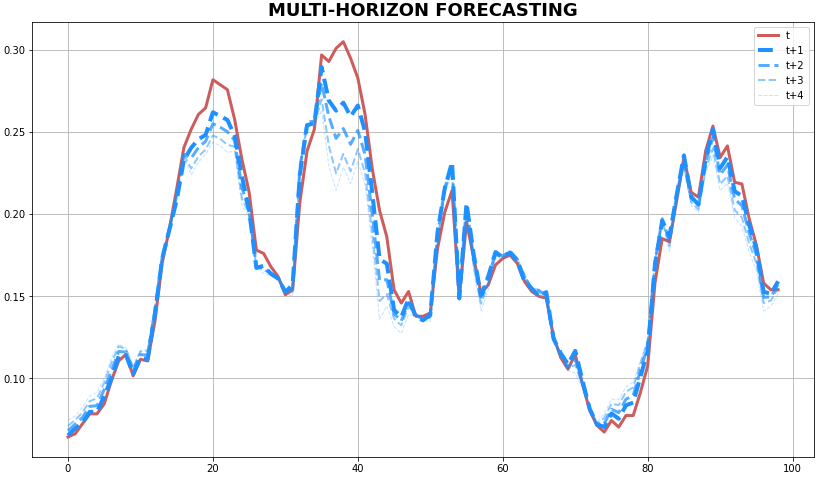
\includegraphics[width=1\textwidth]{multi-horizon-plot.png}
				\caption{Pronóstico de horizonte múltiple.}
				\label{fig:multihorizon_plot}
			\end{center}
		\end{figure}
						
		\begin{table}[H]
			\centering
			\begin{tabular}{ccc}
				\hline
				\texttt{t}   & \texttt{MAE} & \texttt{MASE} \\ \hline
				\texttt{t+1} & 0.00527      & 0.454         \\
				\texttt{t+2} & 0.00728      & 0.628         \\
				\texttt{t+3} & 0.00953      & 0.822         \\
				\texttt{t+4} & 0.01167      & 1.006         \\ \hline
			\end{tabular}
			\caption{Resultados del modelo de horizonte múltiple.}
			\label{tab:multi-horizon-results}
		\end{table}
						
						
						
		\subsubsection{Resultados}
		Se entrenaron los 4 modelos principales (posteriormente se mostrarán los resultados de la \texttt{CNN} causal dilatada, ya que requiere un tratamiento diferente). Los siguientes hiper-parámetros se seleccionaron luego de varios ensayos donde se comprobó que como valores estándar tenían un rendimiento aceptable:
		\begin{itemize}[noitemsep, topsep=2pt]
			\item \texttt{EPOCHS}=200
			\item \texttt{UNITS}=250
			\item \texttt{BATCH\_SIZE}=64
			\item \texttt{T}=8
			\item \texttt{HORIZON}=1
			\item \texttt{CNN\_LAYERS}=3
		\end{itemize}
						
		Se obtuvieron los resultados de la fig.~\ref{fig:training_plot}. Los saltos que observamos en el \texttt{val\_loss} (el más notorio en \texttt{CNNLSTM}) se deben a la callback de \texttt{ReduceLROnPlateau} (sección \ref{plateau}), siendo una función de \textit{Keras} muy provechosa para nuestro objetivo.
						
		\begin{figure}[H]
			\begin{center}
				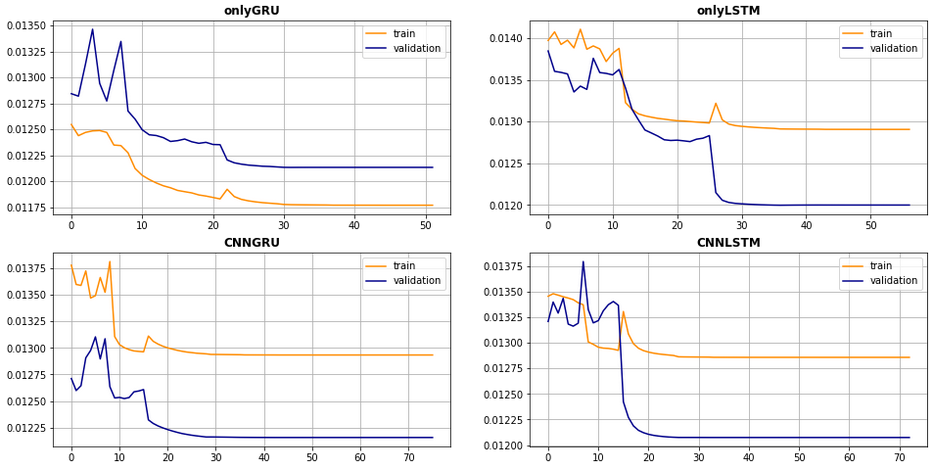
\includegraphics[width=1\textwidth]{training_plots.png}
				\caption{Resultados de entrenamiento de los modelos \texttt{GRU/LSTM}.}
				\label{fig:training_plot}
			\end{center}
		\end{figure}
						
						
						
		Para el entrenamiento de modelos compuestos exclusivamente de capas \texttt{CNN} dilatadas causales se utilizaron los siguientes hiper-parámetros:
		\begin{itemize}[noitemsep, topsep=2pt]
			\item \texttt{KERNEL\_SIZE}=$2$
			\item \texttt{DEEP\_LAYERS}=$1+i$ dónde $i \in \mathbb{N}: 1 \leq i \leq 8$.
			\item \texttt{dilation\_rate}=$i^2$ dónde $i \in \mathbb{N}: 1 \leq i \leq 8$.
		\end{itemize}
						
		En la fig.~\ref{fig:train_cnn} representamos cada uno de los entrenamientos de los modelos, en los cuáles fuimos variando en cada modelo el valor de \texttt{dilation\_rate}.
						
		\begin{figure}[H]
			\begin{center}
				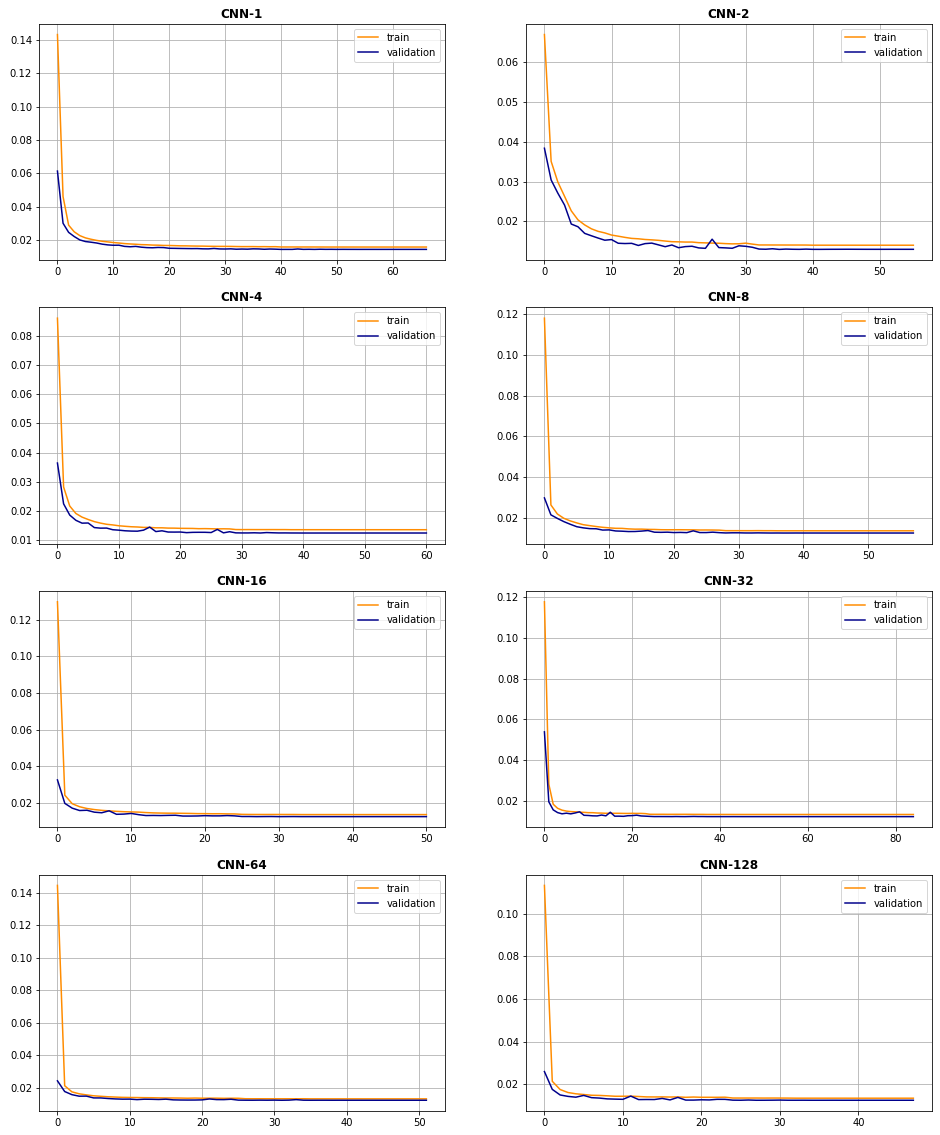
\includegraphics[width=0.9\textwidth]{train_cnn.png}
				\caption{Resultados de entrenamiento de los modelos \texttt{CNN}.}
				\label{fig:train_cnn}
			\end{center}
		\end{figure}
						
		Las diferencias que podemos notar entre la fig.~\ref{fig:training_plot} y la fig.~\ref{fig:train_cnn} es que los modelos que poseen un componente \texttt{RNN} tienden a ser mucho más caóticos en su entrenamiento pero si la cantidad de épocas es suficiente el resultado es satisfactorio. En cambio, los modelos \texttt{CNNs} puros reflejan un entrenamiento más armonioso y continuo.
						
		En la tabla~\ref{tab:metrics-models} y en la fig.~\ref{fig:mase_per_model} verificamos que el modelo con el mejor \texttt{MASE} es el \texttt{CNNGRU}, sin embargo esto lo realizamos con valores fijos y estándares para los hiper-parámetros de los modelos.
						
		\begin{table}[H]
			\centering
			\begin{tabular}{lcc}
				\hline
				\multicolumn{1}{l}{model} & \texttt{MAE}    & \texttt{MASE}   \\ \hline
				\texttt{GRU}              & 0.0121          & 0.2894          \\
				\texttt{LSTM}             & 0.0123          & 0.2777          \\
				\textbf{\texttt{CNNGRU}}  & \textbf{0.0123} & \textbf{0.2775} \\
				\texttt{CNNLSTM}          & 0.0123          & 0.2793          \\
				\texttt{CNN-1}            & 0.0144          & 0.6526          \\
				\texttt{CNN-2}            & 0.0124          & 0.3476          \\
				\texttt{CNN-4}            & 0.0126          & 0.3242          \\
				\texttt{CNN-8}            & 0.0133          & 0.4389          \\
				\texttt{CNN-16}           & 0.0124          & 0.3172          \\
				\texttt{CNN-32}           & 0.0127          & 0.3318          \\
				\texttt{CNN-64}           & 0.0126          & 0.3597          \\
				\texttt{CNN-128}          & 0.0122          & 0.3121          \\ \hline
			\end{tabular}
			\caption{Métricas de los modelos.}
			\label{tab:metrics-models}
		\end{table}
						
		\begin{figure}[H]
			\begin{center}
				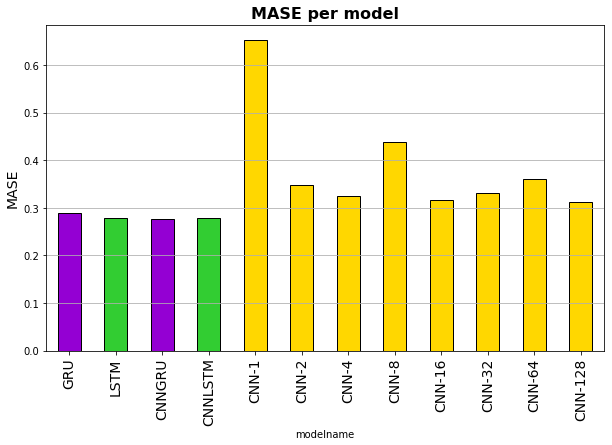
\includegraphics[width=0.65\textwidth]{mase_per_model.png}
				\caption{\texttt{MASE} por modelo.}
				\label{fig:mase_per_model}
			\end{center}
		\end{figure}
						
		Para una mejor visualización de los resultados, en la fig.~\ref{fig:fore_best_model} se toman las 200 primeras muestras. La precisión del modelo es alta, pronosticando valores muy cercanos a los reales. Por tanto, para estos datos el modelo ha resultado eficaz.
						
		\begin{figure}[H]
			\begin{center}
				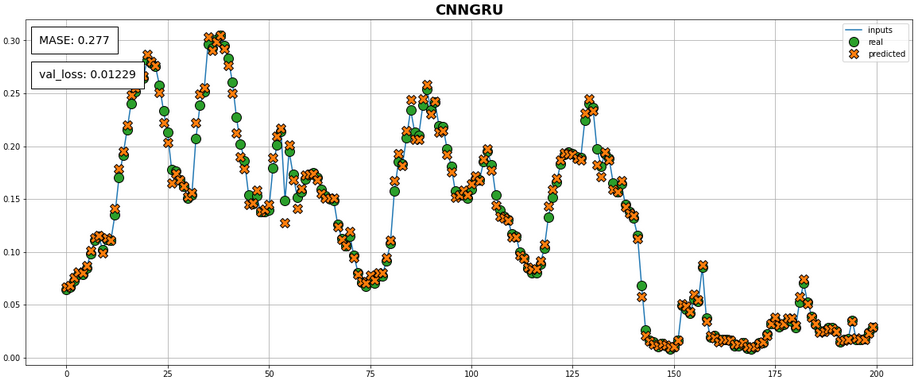
\includegraphics[width=1\textwidth]{cnngru_final.png}
				\caption{Pronóstico del mejor modelo.}
				\label{fig:fore_best_model}
			\end{center}
		\end{figure}
						
						
						
		\subsection{Ajuste de hiperparámetros}
						
		Para obtener el mejor modelo es necesario explorar diversas configuraciones a través del ajuste de hiperparámetros (sección \ref{tuning-hp}).
						
		Para esta labor existen diversas librerías detalladas en la tabla~\ref{tab:comparison-hpo-fws} \citep{neptune}. Entre todas ellos nuestra decisión será \textit{Keras-tuner}, esencialmente por su facilidad de uso con la librería \textit{Keras} (\textit{framework} seleccionada de \textit{Machine Learning}).
						
		\begin{table}[H]
			\centering
			\begin{tabular}{|l|c|c|c|c|c|c|c|c|c|c|}
				\hline
				\multicolumn{1}{|c|}{\multirow{2}{*}{\textbf{\begin{tabular}[c]{@{}c@{}}\textit{Frameworks}\\ HPO\end{tabular}}}} &
				\multicolumn{3}{c|}{\textbf{Algoritmos}} &
				\multicolumn{6}{c|}{\textbf{\textit{Frameworks ML}}} &
				\multirow{2}{*}{GPU} \\ \cline{2-10}
				\multicolumn{1}{|c|}{} &
				\texttt{HB} &
				\texttt{BO} &
				\texttt{RS} &
				\texttt{PT} &
				\texttt{TF} &
				\texttt{SL} &
				\texttt{XGB} &
				\texttt{LGBM} &
				\texttt{MN} &
				\\ \hline
				\textit{Ray Tune}          & Si & Si & No & Si & Si & Si & Si & Si & No & Si                         \\ \hline
				\textit{Optuna}            & Si & Si & No & Si & Si & No & No & No & Si & No                         \\ \hline
				\textit{Hyperopt}          & No & No & Si & Si & Si & Si & Si & No & No & Si                         \\ \hline
				\textit{Scikit-Optimize}   & Si & Si & Si & No & No & Si & No & No & No & No                         \\ \hline
				\textit{Keras-tuner}       & Si & Si & Si & No & Si & No & No & No & No & Si                         \\ \hline
				\textit{Microsoft’s NNI} & No & Si & No & Si & Si & Si & No & No & No & Si                         \\ \hline
			\end{tabular}
			\caption{Comparación de los diferentes \textit{frameworks} disponibles para optimización de hiper-parámetros.}
			\label{tab:comparison-hpo-fws}
		\end{table}
						
		Acŕonimos utilizados:
		\begin{itemize}[noitemsep, topsep=2pt]
			\item \texttt{HB}: \textit{HyperBand}.
			\item \texttt{BO}: \textit{Bayesian Optimization}.
			\item \texttt{RS}: \textit{Random Search}.
			\item \texttt{PT}: \textit{PyTorch}.
			\item \texttt{TF}: \textit{TensorFlow}.
			\item \texttt{SL}: \textit{Scikit-Learn}.
			\item \texttt{XGB}: \textit{XgBoost}.
			\item \texttt{LGBM}: \textit{LightGBM}.
			\item \texttt{MN}: \textit{MxNet}.	
		\end{itemize}
						
		\subsubsection{\textit{Keras-tuner}}
		La librería se compone de diversas clases y métodos que nos permitirán ajustar los hiperparámetros de nuestros modelos creados en \textit{Keras}. \citep{keras-tuner}
						
		\textbf{Clase \texttt{HyperParameters}}
						
		Sirve como contenedor de hiperparámetros, una instancia de \texttt{HyperParameters} contiene información sobre el espacio de búsqueda y los valores actuales de cada hiperparámetro.
						
						
						
		Además nos provee diversos métodos para decidir de que manera queremos explorar el espacio de búsqueda de un determinado hiperparámetro:
						
		\begin{itemize}[noitemsep, topsep=2pt]
			\item \texttt{Boolean}: elige entre \texttt{True} o \texttt{False}.
			\item \texttt{Choice}: elige entre una lista de opciones.
			\item \texttt{Fixed}: fijo, no permite cambiar su valor.
			\item \texttt{Int}: explora números enteros entre el valor inicial y final, es posible seleccionar el modo y el paso.
			\item \texttt{Float}: \textit{ídem} al ítem anterior, pero con números reales.
		\end{itemize}
						
		\textbf{Clase \texttt{Oracle}}
						
		Cada clase \texttt{Oracle} (óraculo) implementa un algoritmo de ajuste de hiperparámetros particular. Un \texttt{Oracle} se pasa como argumento a un \texttt{Tuner} (clase cuyo objetivo es realizar la búsqueda de hiperpárametros). \texttt{Oracle} le informa al \texttt{Tuner} qué hiperparámetros deben probarse a continuación.
						
		La mayoría de las clases de \texttt{Oracle} se pueden combinar con cualquier subclase de \texttt{Tuner} definida por el usuario. Si no se necesita una subclase de \texttt{Tuner} (el caso más común), también se proporciona una serie de clases que empaquetan un \texttt{Tuner} y un \texttt{Oracle} juntos (cómo veremos a continuación).
						
		\textbf{Clase \texttt{Tuner}}
						
		Su propósito es realizar la búsqueda de hiperparámetros en el espacio de búsqueda definido, y como se aclaró en la sección anterior es posible crearlos de forma personalizada pero los algoritmos ofrecidos son más que suficientes para nuestra tarea (analizados en la sección \ref{algo-hp}):
		\begin{itemize}[noitemsep, topsep=2pt]
			\item Búsqueda Aleatoria (descartado).
			\item Optimización Bayesiana: parámetro a destacar:
			      \begin{itemize}[noitemsep, topsep=2pt]
			      	\item \texttt{max\_trials}: número total de pruebas (configuraciones de modelo) para probar como máximo.
			      \end{itemize}
			\item \textit{Hyperband}: parámetros a destacar:
			      \begin{itemize}[noitemsep, topsep=2pt]
			      	\item \texttt{factor}: factor de reducción ($\eta$) para el número de épocas y el número de modelos para cada \texttt{bracket}.
			      	\item \texttt{hyperband\_iterations}: el número de veces que se iterará sobre el algoritmo \textit{Hyperband} completo. Una iteración ejecutará aproximadamente $s_{max}(\log_{\eta} s_{max})^2$ épocas acumulativas en todas las pruebas (notación tomada de la sección \ref{hyperband}). Se recomienda establecer esto en un valor tan alto como esté dentro de su presupuesto de recursos.
			      \end{itemize}
		\end{itemize}
						
						
						
		\subsubsection{Espacio de búsqueda}
		Para cada tipo de modelo se definió un espacio de búsqueda determinado en función a su arquitectura.
						
		\textbf{\texttt{RNN}}
						
		Se limitó a explorar la cantidad de unidades en las capas recurrentes e intercambiar la función de activación de la capa final.
						
		\begin{python}
			# RNN layer
			for i in range(8,256,16):
			units = i
			# Dense layer
			for j in ['relu', 'sig', 'tanh']:
			dense = j
		\end{python}
						
		\textbf{\texttt{CNN}}
						
		En este caso se debió crear una capa \texttt{CNN} \textit{input} y sobre la misma ir apilando las demás capas \texttt{CNN} que fueron variando en cantidad desde 1 a 3.
		Además se ajustaron los hiperpárametros de filtros y tamaño del kernel en cada una de ellas.
						 
		\begin{python}
			# For first layer
			for i in range(8,64,16):
			filters_0 = i
			for j in range(2,8,2):
			kernel_size_0
									
			# Others layers
			for i in range(1,3):
			cnn_i = stack_cnnlayer(dilation_date=2**i)
			for j in range(8,64,16):
			filters_i = j
			for k in range(2,8,2):
			kernel_size_i = k
									
			# Model compile
			for lr in [1e-2, 1e-3, 1e-4]:
			model_lr = lr
		\end{python}
						
						
						
		\textbf{\texttt{CNNRNN}}
						
		Se realizó una configuración mixta de los hiperparámetros de las otras arquitecturas, dónde la única novedad es la búsqueda en los hiperparámetros de la capa \texttt{MaxPooling1D}.
						
		\begin{python}
			# First CNN layer
			for i in range(8,64,16):
			filters_0 = i
			for j in range(2,8,2):
			kernel_size_0
									
			# Others CNN layers
			for i in range(1,3):
			cnn_i = stack_cnnlayer(dilation_date=2**i)
			for j in range(8,64,16):
			filters_i = j
			for k in range(2,8,2):
			kernel_size_i = k
												
			# Pooling layer
			for i in range(2,8,2):
			pool_size = i
										
			# RNN layer
			for i in range(8,256,16):
			units = i
										
			# Model compile
			for lr in [1e-2, 1e-3, 1e-4]:
			model_lr = lr
		\end{python}
						
						
						
		\subsubsection{Resultados \textit{dataset} polución}
						
		Ya definido el espacio de búsqueda de los modelos, se procede a la búsqueda del mejor conjunto de hiperparámetros obteniendo la tabla \ref{tab:tuning-hp} (recordar que se utiliza como métrica \texttt{MAE}). De la misma podemos sacar varias conclusiones interesantes.
		\begin{itemize}[noitemsep, topsep=2pt]
			\item El modelo con la mejor puntuación fue \texttt{CNNGRU} en combinación con el algoritmo \textit{Hyperband},aunque el segundo lugar (\texttt{LSTM}/Optimización Bayesiana) le sigue muy de cerca. De hecho todos los modelos están muy parejos.
			\item Hay una clara tendencia a obtener mejores resultados con combinaciones definidas como \texttt{CNNGRU/HB/sig} y \texttt{LSTM/BO/tanh}.
			\item Es interesante notar que a pesar de su arquitectura simple \texttt{LSTM} logró batir los resultados de otros modelos.
			\item Nuestro tope de unidades \texttt{RNN} fue seteado en 256, observamos que los modelos con mejor puntaje están muy cerca de ese valor. Existe la posibilidad de obtener mejores resultados en caso de haber definido un espacio de búsqueda mayor para ese hiperparámetro.
		\end{itemize}
						
		\begin{table}[H]
			\centering
			\begin{adjustwidth}{-1.3cm}{}
				\begin{tabular}{lcccccccccccc}
					\hline
					\textbf{}       & \textbf{}               & \multicolumn{7}{c}{\texttt{CNN}} & \texttt{MAXPOOL} & \texttt{RNN} & \texttt{DENSE}                  & \textbf{} \\ \hline
					\multicolumn{1}{c}{model} &
					\multicolumn{1}{c|}{algo} &
					layers &
					$f_0$ &
					$ks_0$ &
					$f_1$ &
					$ks_1$ &
					$f_2$ &
					$ks_2$ &
					$ps$ &
					units &
					\multicolumn{1}{c|}{act} &
					\textbf{score} \\ \hline
					\texttt{CNNGRU} & \multicolumn{1}{c|}{\texttt{HB}} & 3 & 40 & 8 & 56 & 4 & 56 & 6 & 6 & 232             & \multicolumn{1}{c|}{\texttt{sig}}  & 0.011961 \\
					\texttt{LSTM}   & \multicolumn{1}{c|}{\texttt{BO}} & - & -  & - & -  & - & -  & - & - & 248             & \multicolumn{1}{c|}{\texttt{tanh}} & 0.011973 \\
					\texttt{CNNGRU} & \multicolumn{1}{c|}{\texttt{HB}} & 3 & 40 & 8 & 56 & 4 & 56 & 6 & 6 & 232             & \multicolumn{1}{c|}{\texttt{sig}}  & 0.011980 \\
					\texttt{LSTM}   & \multicolumn{1}{c|}{\texttt{BO}} & - & -  & - & -  & - & -  & - & - & 248             & \multicolumn{1}{c|}{\texttt{tanh}} & 0.011996 \\
					\texttt{CNNGRU} & \multicolumn{1}{c|}{\texttt{HB}} & 3 & 40 & 8 & 56 & 4 & 56 & 6 & 6 & 232             & \multicolumn{1}{c|}{\texttt{sig}}  & 0.011996 \\
					\texttt{LSTM}   & \multicolumn{1}{c|}{\texttt{BO}} & - & -  & - & -  & - & -  & - & - & 248             & \multicolumn{1}{c|}{\texttt{tanh}} & 0.012001 \\
					\texttt{CNNGRU} & \multicolumn{1}{c|}{\texttt{HB}} & 1 & 56 & 6 & -  & - & -  & - & 6 & 88              & \multicolumn{1}{c|}{\texttt{sig}}  & 0.012003 \\
					\texttt{LSTM}   & \multicolumn{1}{c|}{\texttt{BO}} & - & -  & - & -  & - & -  & - & - & 248             & \multicolumn{1}{c|}{\texttt{tanh}} & 0.012004 \\
					\texttt{CNNGRU} & \multicolumn{1}{c|}{\texttt{HB}} & 1 & 40 & 6 & -  & - & -  & - & 6 & 120             & \multicolumn{1}{c|}{\texttt{sig}}  & 0.012004 \\
					\texttt{CNNGRU} & \multicolumn{1}{c|}{\texttt{HB}} & 2 & 40 & 6 & 40 & 4 & -  & - & 6 & 216             & \multicolumn{1}{c|}{\texttt{sig}}  & 0.012008 \\ \hline
				\end{tabular}
			\end{adjustwidth}
			\caption{Resultados del ajuste de hiperpárametros.}
			\label{tab:tuning-hp}
		\end{table}
						
		Se pondrá atención en los rendimientos por arquitectura de ambos algoritmos de ajuste de hiperparámetros utilizados discriminando los análisis por las dos métricas propuestas (\texttt{MAE} y \texttt{MASE}). 
						
						
						
		\textbf{\texttt{MAE}}
						
		Notamos que exceptuando \texttt{LSTM}, el algoritmo \textit{Hyperband} se desempeña mejor en cada uno de los modelos restantes (tabla~\ref{tab:algo_vs_arch_mae} y fig.~\ref{fig:algo_comparison_mae}).
						
		\begin{table}[H]
			\centering
			\begin{tabular}{l|ccccc}
				\hline
				algo/model                    & \texttt{CNN} & \texttt{CNNGRU} & \texttt{CNNLSTM} & \texttt{GRU} & \texttt{LSTM} \\ \hline
				\textit{BayesianOptimization} & 0.01260      & 0.01224         & 0.01222          & 0.01218      & 0.01197       \\
				\textit{Hyperband}            & 0.01213      & 0.01196         & 0.01203          & 0.01204      & 0.01202       \\ \hline
			\end{tabular}
			\caption{Mejor puntuación por algoritmo y arquitectura utilizando \texttt{MAE} cómo métrica.}
			\label{tab:algo_vs_arch_mae}
		\end{table}
						
		\begin{figure}[H]
			\begin{center}
				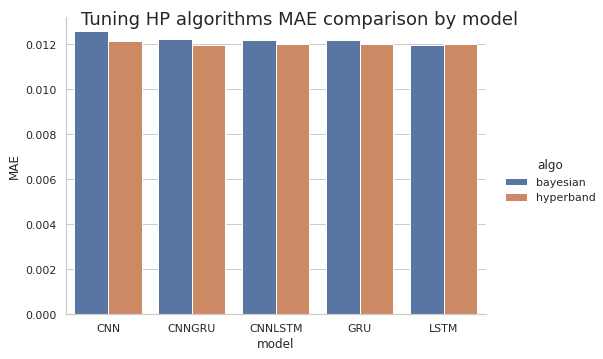
\includegraphics[width=0.8\textwidth]{model_vs_algo_hp_mae.png}
				\caption{Comparación de algoritmos de ajuste de hiperpárametros por modelo y arquitectura utilizando como métrica \texttt{MAE}.}
				\label{fig:algo_comparison_mae}
			\end{center}
		\end{figure}
						
						
						
		\textbf{\texttt{MASE}}
						
		Es arduo crear una función de pérdida \texttt{MASE} ya que ésta recibe como parámetro muestras previas, añadiendo una complejidad que no fue posible superar en su implementación (\textit{Keras} no soportaba esta característica). En consecuencia utilizamos \texttt{MAE} cómo métrica para entrenar nuestros modelos, sin embargo \texttt{MASE} es nuestra principal métrica a la hora de definir cual es el mejor modelo para el objetivo propuesto.
						
		Concluimos que la combinación que posee el mejor rendimiento en nuestro \textit{set} de datos es \texttt{CNN} con Optimización Bayesiana (tabla~\ref{tab:algo_vs_arch_mase} y fig.~\ref{fig:algo_comparison_mase}).
						
		\begin{table}[H]
			\centering
			\begin{tabular}{l|ccccc}
				\hline
				algo/model                    & \texttt{CNN} & \texttt{CNNGRU} & \texttt{CNNLSTM} & \texttt{GRU} & \texttt{LSTM} \\ \hline
				\textit{BayesianOptimization} & 0,208        & 0,300           & 0,306            & 0,243        & 0,297         \\
				\textit{Hyperband}            & 0,253        & 0,332           & 0,290            & 0,628        & 0,304         \\ \hline
			\end{tabular}
			\caption{Mejor resultado por algoritmo y arquitectura utilizando como métrica \texttt{MASE}.}
			\label{tab:algo_vs_arch_mase}
		\end{table}
						
		\begin{figure}[H]
			\begin{center}
				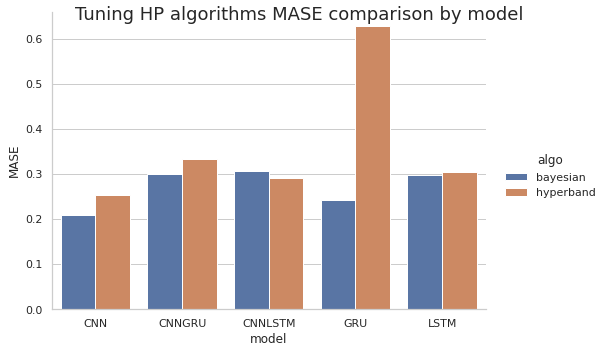
\includegraphics[width=0.8\textwidth]{model_vs_algo_hp_mase.png}
				\caption{Comparación de algoritmos de ajuste de hiperpárametros por modelo y arquitectura utilizando como métrica \texttt{MAE}.}
				\label{fig:algo_comparison_mase}
			\end{center}
		\end{figure}
						
						
						
		En la fig.~\ref{fig:best_model_hp} podemos notar la excelente precisión del modelo al predecir los instantes \texttt{t+1}, justificando de manera visual el análisis realizado.
						
		\begin{figure}[H]
			\begin{center}
				\includegraphics[width=1\textwidth]{cnn_bo_best.png}
				\caption{Pronóstico del mejor modelo una vez realizado el ajuste de hiperparámetros.}
				\label{fig:best_model_hp}
			\end{center}
		\end{figure}
						
		Para destacar la utilidad del ajuste de hiperparámetros recordemos la tabla~\ref{tab:metrics-models}. En la misma notamos que el mejor modelo (\texttt{CNNGRU}) logró un \texttt{MASE} de $0.278$ mientras que el modelo (\texttt{CNN}) de mejor rendimiento una vez aplicado el ajuste de hiperparámetros obtuvo $0.208$, una mejora de casi 8 puntos. También es interesante notar que antes del ajuste de hiperpárametros los modelos \texttt{CNN} estaban muy lejos de los mejores rendimientos, pero luego se posicionaron como la mejor opción.
						
		\subsubsection{Conclusión}
		Si bien el ajuste de hiperparámetros es más costoso computacionalmente que el entrenamiento de los modelos, si la necesidad radica en obtener el mejor modelo posible con nuestros recursos definitivamente es un paso indispensable.
						
						
						
		\subsubsection{Resultados \textit{dataset} FSI}
		Los mismos procedimientos realizados sobre nuestra \textit{dummy data} serán aplicados a nuestro \textit{dataset} de \texttt{FSI}.
						
		Los modelos obtenidos sin búsqueda de hiperparámetros arrojan los resultados de la tabla~\ref{tab:score_table_fsi} que son interpretados visualmente en la fig.~\ref{fig:mase_per_model_fsi}. Si comparamos los gráficos entre ambos \textit{datasets}, tenemos un rendimiento 8 veces peor en promedio (\texttt{MAE}) que con el \textit{dataset} de polución, esto claramente repercutirá en la precisión de pronóstico de nuestros modelos.
						
		\begin{table}[H]
			\centering
			\begin{tabular}{lcc}
				\hline
				\multicolumn{1}{c}{{model}} & \multicolumn{1}{c}{\texttt{val\_loss}} & \multicolumn{1}{c}{\texttt{MASE}} \\ \hline
				\texttt{GRU}                & 0.0874                                 & 0.7308                            \\
				\texttt{LSTM}               & 0.0891                                 & 0.8138                            \\
				\texttt{CNNGRU}             & 0.0865                                 & 0.6575                            \\
				\texttt{CNNLSTM}            & 0.0841                                 & 0.7877                            \\
				\texttt{CNN-1}              & 0.0867                                 & 0.6812                            \\
				\texttt{CNN-2}              & 0.0891                                 & 0.6949                            \\
				\texttt{CNN-4}              & 0.0888                                 & 0.7675                            \\
				\texttt{CNN-8}              & 0.0844                                 & 0.6984                            \\
				\texttt{CNN-16}             & 0.0846                                 & 0.6260                            \\
				\texttt{CNN-32}             & 0.0839                                 & 0.7574                            \\
				\texttt{CNN-64}             & 0.0847                                 & 0.6516                            \\
				\texttt{CNN-128}            & 0.0878                                 & 0.7501                            \\ \hline
			\end{tabular}
			\caption{Métricas de los modelos para el \textit{dataset} FSI.}
			\label{tab:score_table_fsi}
		\end{table}
						
		\begin{figure}[H]
			\begin{center}
				\includegraphics[width=0.63\textwidth]{mase_per_model_fsi.png}
				\caption{\texttt{MASE} por modelo con \textit{dataset} FSI.}
				\label{fig:mase_per_model_fsi}
			\end{center}
		\end{figure}
						
		El mejor modelo con un \texttt{MASE} de 0.626 es \texttt{CNN-16} seguido de cerca por \texttt{CNNGRU}. Se observa que los modelos \texttt{LSTM} funcionan peor que los demás pero no podemos sacar conclusiones claras aún.
						
		De la fig.~\ref{fig:best_model_fsi} notamos que a nuestro modelo no tiene problemas en predecir mínimos pero le es casi imposible predecir máximos debido a los cambios abruptos de la serie temporal.
						
		\begin{figure}[H]
			\begin{center}
				\includegraphics[width=1\textwidth]{best_model_fsi.png}
				\caption{Mejor modelo para el \textit{dataset} FSI.}
				\label{fig:best_model_fsi}
			\end{center}
		\end{figure}
						
		Obtenemos la tabla \ref{tab:tuning-hp} (recordar que se utiliza como métrica \texttt{MAE}). De la misma podemos sacar varias conclusiones interesantes.
		\begin{itemize}[noitemsep, topsep=2pt]
			\item El modelo con la mejor puntuación fue \texttt{CNNGRU} en combinación con el algoritmo \textit{HyperBand}, y en segundo lugar (\texttt{LSTM}/\textit{HyperBand}) apenas por detrás.
			\item 2 capas de \texttt{CNN} fueron suficientes, e incluso podría haberse utilizado solo una.
			\item Las unidades de las capas \texttt{RNN} varían demasiado sin definir un rango de valores claros.
			\item Sin lugar a dudas la mejor función de activación fue la sigmoide.
		\end{itemize}
						
		\hfill
						
		\begin{table}[H]
			\centering
			\begin{adjustwidth}{-1.3cm}{}
				\begin{tabular}{lcccccccccccc}
					\hline
					& \multicolumn{1}{l}{}    & \multicolumn{7}{c}{\texttt{CNN}}      & \texttt{MAXPOOL} & \texttt{RNN} & \texttt{DENSE}   &          \\ \hline
					\multicolumn{1}{c}{{model}} &
					\multicolumn{1}{c|}{{algo}} &
					{layers} &
					\multicolumn{1}{c}{{$f_0$}} &
					\multicolumn{1}{c}{{$ks_0$}} &
					\multicolumn{1}{c}{{$f_1$}} &
					\multicolumn{1}{c}{{$ks_1$}} &
					\multicolumn{1}{c}{{$f_2$}} &
					\multicolumn{1}{c}{{$ks_2$}} &
					{$p_s$} &
					{units} &
					{act} &
					{score} \\ \hline
					\texttt{CNNGRU}  & \multicolumn{1}{c|}{\texttt{HB}} & 1 & 56 & 4 & 24 & 6 & 40 & 4 & 6 & 120              & \texttt{sig}                     & 0.080426 \\
					\texttt{CNNGRU}  & \multicolumn{1}{c|}{\texttt{HB}} & 2 & 56 & 4 & 40 & 4 & 40 & 4 & 6 & 200              & \texttt{sig}                     & 0.080560 \\
					\texttt{CNNLSTM} & \multicolumn{1}{c|}{\texttt{HB}} & 2 & 56 & 2 & 56 & 6 & 24 & 6 & 4 & 168              & \texttt{sig}                     & 0.080621 \\
					\texttt{CNNGRU}  & \multicolumn{1}{c|}{\texttt{HB}} & 1 & 56 & 6 & 24 & 6 & 56 & 6 & 8 & 184              & \texttt{sig}                     & 0.080632 \\
					\texttt{CNNLSTM} & \multicolumn{1}{c|}{\texttt{HB}} & 1 & 40 & 8 & 24 & 4 & 24 & 6 & 8 & 232              & \texttt{sig}                     & 0.080693 \\
					\texttt{CNNLSTM} & \multicolumn{1}{c|}{\texttt{HB}} & 1 & 24 & 4 & 56 & 4 & 24 & 8 & 6 & 152              & \texttt{sig}                     & 0.080752 \\
					\texttt{CNNLSTM} & \multicolumn{1}{c|}{\texttt{HB}} & 1 & 56 & 6 & 56 & 2 & 56 & 4 & 8 & 248              & \texttt{sig}                     & 0.080915 \\
					\texttt{CNNLSTM} & \multicolumn{1}{c|}{\texttt{HB}} & 1 & 24 & 4 & 40 & 6 & 24 & 4 & 6 & 184              & \texttt{sig}                     & 0.080979 \\
					\texttt{CNNGRU}  & \multicolumn{1}{c|}{\texttt{HB}} & 2 & 56 & 6 & 24 & 4 & 56 & 4 & 8 & 248              & \texttt{sig}                     & 0.081028 \\
					\texttt{CNNGRU}  & \multicolumn{1}{c|}{\texttt{HB}} & 1 & 40 & 8 & 40 & 2 & 8  & 6 & 8 & 200              & \texttt{sig}                     & 0.081080 \\ \hline
				\end{tabular}
			\end{adjustwidth}
			\caption{Resultados de ajuste de hiperpárametros del \textit{dataset} FSI.}
			\label{tab:tuning-hp-fsi}
		\end{table}
						
		\textbf{\texttt{MAE}}
						
		Para esta tarea utilizaremos de soporte la tabla~\ref{tab:algo_vs_arch_mae_fsi} y la fig.~\ref{fig:algo_comparison_mae_fsi}. Excepto \texttt{GRU},\textit{Hyperband} obtiene un mejor rendimiento en cada uno de los modelos restantes.
						
		\begin{table}[H]
			\centering
			\begin{tabular}{l|ccccc}
				\hline
				algo/model                    & \texttt{CNN} & \texttt{CNNGRU} & \texttt{CNNLSTM} & \texttt{GRU} & \texttt{LSTM} \\ \hline
				\textit{BayesianOptimization} & 0.08309      & 0.08138         & 0.08138          & 0.08558      & 0.08346       \\
				\textit{Hyperband}            & 0.08196      & 0.08043         & 0.08062          & 0.09082      & 0.08389       \\ \hline
			\end{tabular}
			\caption{Mejor puntuación por algoritmo y arquitectura utilizando \texttt{MAE} cómo métrica en \textit{dataset} FSI.}
			\label{tab:algo_vs_arch_mae_fsi}
		\end{table}
						
		\begin{figure}[H]
			\begin{center}
				\includegraphics[width=0.67\textwidth]{model_vs_algo_hp_mae_fsi.png}
				\caption{Comparación de algoritmos de ajuste de hiperpárametros por modelo y arquitectura utilizando como métrica \texttt{MAE}.}
				\label{fig:algo_comparison_mae_fsi}
			\end{center}
		\end{figure}
						
		\textbf{\texttt{MASE}}
						
		Utilizando la tabla~\ref{tab:algo_vs_arch_mase_fsi} y la fig.~\ref{fig:algo_comparison_mase_fsi} concluimos que la combinación que posee el mejor rendimiento en nuestro \textit{set} de datos es \texttt{CNN} con \textit{HyperBand}. En el \textit{dataset} de polución el mejor rendimiento también se obtuvo a través de una \texttt{CNN} pero el algoritmo de ajuste de hiperparámetros fue \textit{Bayesian}. Aunque en nuestros dos \textit{datasets} hayamos obtenido que el mejor modelo es \texttt{CNN} no se puede asegurar que no habrá arquitecturas que funcionen mejor con otras series temporales.
						
		\begin{table}[H]
			\centering
			\begin{tabular}{l|ccccc}
				\hline
				algo/model                    & \texttt{CNN} & \texttt{CNNGRU} & \texttt{CNNLSTM} & \texttt{GRU} & \texttt{LSTM} \\ \hline
				\textit{BayesianOptimization} & 0.661        & 0.659           & 0.707            & 0.730        & 0.754         \\
				\textit{Hyperband}            & 0.627        & 0.707           & 0.704            & 0.744        & 0.752         \\ \hline
			\end{tabular}
			\caption{Mejor resultado por algoritmo y arquitectura utilizando como métrica \texttt{MASE} en \textit{dataset} FSI.}
			\label{tab:algo_vs_arch_mase_fsi}
		\end{table}
						
		\begin{figure}[H]
			\begin{center}
				\includegraphics[width=0.67\textwidth]{model_vs_algo_hp_mase_fsi.png}
				\caption{Comparación de algoritmos de ajuste de hiperpárametros por modelo y arquitectura utilizando como métrica \texttt{MASE} para el \textit{dataset} FSI.}
				\label{fig:algo_comparison_mase_fsi}
			\end{center}
		\end{figure}
						
		En la fig.~\ref{fig:cnn_hp_best_fsi} resaltamos lo antes mencionado, nuestro modelo carece de la capacidad de predecir los valores máximos de la función, pero puede predecir los valores mínimos. Si pensamos a cada capa como un amplificador podemos intuir que quizás una de las mismas se esté saturando incapacitando a las siguientes a llegar a los valores máximos. Se realizará un análisis ajustando los datos de entrada al modelo con diferentes \textit{scalers}. %(con la intención de cambiar la amplitud de la señal que ingresa a la red para ver si así logramos predecir los valores a los cuales no estamos llegando).
						
		\begin{figure}[H]
			\begin{center}
				\includegraphics[width=1\textwidth]{cnn_hp_best_fsi.png}
				\caption{Pronóstico del mejor modelo para el \textit{dataset} FSI una vez realizado el ajuste de hiperparámetros.}
				\label{fig:cnn_hp_best_fsi}
			\end{center}
		\end{figure}
						
		Este inconveniente lo hace disfuncional a nuestra tarea pero en la próxima sección intentaremos descubrir que diferencia a ambos \textit{datasets} para que uno funcione tan bien y el otro no.
						
		Comparemos los valores antes y después del ajuste de hiperparámetros, en la tabla~\ref{tab:score_table_fsi} obtuvimos con \texttt{CNN-16} un \texttt{MASE} de 0.626 y la tabla~\ref{tab:algo_vs_arch_mase_fsi} nos dice que el mejor modelo fue un \texttt{CNN} con \texttt{MASE} de 0.627 \textit{i.e.} valores casi idénticos pero además peores para el post-ajuste. 
						
		\subsubsection{Cambio en preprocesamiento de datos}
		Como mencionamos anteriormente, para evitar la saturación en nuestra red variaremos forma en que la misma recibe nuestro \textit{dataset} modificando dos parámetros:
		\begin{itemize}[noitemsep, topsep=2pt]
			\item \textit{Scaler}: algoritmo de preprocesamiento de datos cuyo objetivo usualmente es lograr un \textit{dataset} más homogéneo y sin \textit{outliers}.
			\item Factor de escala ($s_f$): simplemente multiplicaremos toda la red por este valor para obtener amplitudes menores.
		\end{itemize}
						
						
						
		\textit{Scikit-learn} nos provee de varios \textit{scalers} pero seleccionamos los siguientes:
		\begin{itemize}[noitemsep, topsep=2pt]
			\item \texttt{MinMax}: escala cada característica individualmente de modo que se encuentre en el rango seleccionada (\textit{e.g.} 1 y 0).
			\item \texttt{PowerTransformer}: aplica una transformación de potencia en función de las características para hacer que los datos sean más \textit{gaussianos}.
			\item \texttt{RobustScaler}: escala características usando estadísticas que sean robustas a \textit{outliers}.
			\item \texttt{StandardScaler}: estandariza las características eliminando la media y escalando a la varianza unitaria.
		\end{itemize}
						
		Para el factor de escala se definió un rango entre 0.01 y 0.40 tras varios ensayos.
						
		En la tabla~\ref{tab:scalers-table} se corrobora que el \textit{scaler} de mejor rendimiento es\texttt{PowerTransformer} (notar los bajos valores de $s_f$). Con respecto a nuestros resultados originales (en \texttt{MASE}) se obtienen casi 5 puntos de mejora.
						
		\begin{table}[H]
			\centering
			\begin{tabular}{lccc}
				\hline
				\multicolumn{1}{c}{\textit{scaler}} & $s_f$ & \texttt{model} & \texttt{MASE} \\ \hline
				\texttt{PowerTransformer}           & 0.075 & \texttt{GRU}   & 0.5749        \\
				\texttt{PowerTransformer}           & 0.088 & \texttt{GRU}   & 0.5836        \\
				\texttt{PowerTransformer}           & 0.101 & \texttt{GRU}   & 0.5868        \\
				\texttt{PowerTransformer}           & 0.062 & \texttt{GRU}   & 0.5873        \\
				\texttt{PowerTransformer}           & 0.114 & \texttt{GRU}   & 0.5907        \\
				\texttt{PowerTransformer}           & 0.049 & \texttt{GRU}   & 0.6004        \\
				\texttt{PowerTransformer}           & 0.101 & \texttt{LSTM}  & 0.6070        \\
				\texttt{PowerTransformer}           & 0.114 & \texttt{LSTM}  & 0.6128        \\
				\texttt{PowerTransformer}           & 0.127 & \texttt{GRU}   & 0.6142        \\
				\texttt{PowerTransformer}           & 0.088 & \texttt{LSTM}  & 0.6194        \\ \hline
			\end{tabular}
			\caption{Top 10 de mejores \textit{scalers} según \texttt{MASE} obtenido.}
			\label{tab:scalers-table}
		\end{table}
						
		Los modelos \texttt{RNN} puros funcionan mucho mejor que los que poseen algún componente \texttt{CNN} (fig.~\ref{fig:scalers}), una posibilidad es que las capas \texttt{CNN} se sobrecarguen haciendo que el modelo diverja. Además según el \textit{scaler} hay determinadas zonas de valle en las cuales los modelos funcionan mejor. Lo recomendable sería una vez determinado el mejor par \textit{scaler}-zona de mayor rendimiento, explorar utilizando ajuste de hiperparámetros.
						
		\begin{figure}[H]
			\begin{center}
				\includegraphics[width=1\textwidth]{scalers.png}
				\caption{Factor de escala \textit{vs} \texttt{MASE} según \textit{scaler}.}
				\label{fig:scalers}
			\end{center}
		\end{figure}
						
		Los resultados son esclarecedores, si bien seguimos sin llegar a los picos ahora al menos nos aproximamos (fig.~\ref{fig:powertrafo_forecast}) y no tenemos ese techo que no nos permitía escalar (fig.~\ref{fig:cnn_hp_best_fsi}). Otra manera de mejorar el rendimiento de nuestros modelos puede ser variar las configuraciones del preprocesamiento de los datos. Sin embargo esto es tedioso y arduo de automatizar.
						
		\begin{figure}[H]
			\begin{center}
				\includegraphics[width=1\textwidth]{powertrafo_forecast.png}
				\caption{Prónostico utilizando como \textit{scaler} \texttt{PowerTransformer} y modelo \texttt{GRU}.}
				\label{fig:powertrafo_forecast}
			\end{center}
		\end{figure}
						
		\subsubsection{Conclusión}
		No siempre aplicar ajuste de hiperparámetros nos dará resultados mejores a los originales, ya que esto dependerá de cada serie temporal a pronosticar. Pero si intuimos lo que puede estar sucediendo en la red podemos desarrollar soluciones innovadoras.
						
						
						
		\subsection{\href{https://github.com/GeraCollante/tesis-icomp-machinelearning/blob/main/EntropyModel.ipynb}{\color{blue}Entropía}}
		Intentaremos encontrar una causa al dispar rendimiento entre nuestro \textit{dataset} de polución del aire y el de defectos. Para ello haremos uso de lo revisado en la sección~\ref{sec:entropy}, dónde mencionamos que la entropía de los datos influye directamente en la capacidad de predicción de nuestros modelos. Mientras más entropía tengan los datos, más difícil será que el modelo pueda aprender correctamente sus patrones, si es que los hubiere.
						
		Ambos \textit{datasets} serán procesados por los dos algoritmos disponibles para esta tarea: $\textrm{ApEn}$ y $\textrm{SampEn}$.
						
		\subsubsection{Rendimiento de los algoritmos}
		Al realizar los ensayos quedó al descubierto la demora de los algoritmos para ejecutar los cálculos sobre la totalidad del \textit{dataset}, lo que llevó a buscar una solución. \textit{Python} por defecto no posee librerías que hagan uso intensivo de \texttt{GPU} (un caso es \textit{scikit sk-learn}, que a pesar de brindar diversos algoritmos de Aprendizaje Automático sólo utiliza \texttt{CPU} para sus cálculos) y \texttt{NumPy} (librería por defecto para operaciones matriciales y tensoriales) no es la excepción.
						
		\textbf{\texttt{CuPy}}
						
		Es una biblioteca de matrices de código abierto que proporciona computación acelerada por \texttt{GPU} con \textit{Python} a través de \texttt{CUDA}. \citep{CuPy} 
						
		\texttt{CUDA} es una plataforma de computación paralela y un modelo de programación desarrollado por \textit{Nvidia} para computación general en unidades de procesamiento gráfico (\texttt{GPU}). Con \texttt{CUDA}, los desarrolladores pueden acelerar drásticamente las aplicaciones informáticas aprovechando la potencia de las \texttt{GPU}. \citep{CUDA} La implementación de \texttt{CuPy} sobre código creado para la librería \texttt{NumPy} es muy simple.\\
						
		\textbf{Comparación de rendimiento}
						
		Se divisa que a medida que la cantidad de muestras aumenta, el tiempo de ejecución de \texttt{NumPy} crece exponencialmente en contraste con \texttt{CuPy} que crece de forma lineal (fig.~\ref{fig:np_vs_cp} ). En el caso límite que el algoritmo utiliza la totalidad del \textit{dataset} llegamos a tener un \textit{speedup} de \texttt{8X}. Por tanto concluimos que \texttt{CuPy} promete lo que cumple.
						
		\begin{figure}[H]
			\begin{center}
				\includegraphics[width=1\textwidth]{numpy_vs_cupy.png}
				\caption{Comparación de \texttt{NumPy} \textit{vs} \texttt{CuPy}.}
				\label{fig:np_vs_cp}
			\end{center}
		\end{figure}
						
		\subsubsection{\textit{Dataset} de polución}
		Vamos a calcular $\textrm{ApEn}$ y $\textrm{SampEn}$ sobre el \textit{dataset} de polución con $0 \leq m \leq 4$ y y $0 \leq r \leq 0.25$ (recordar que éste valor debe ser multiplicado por la desviación estándar de la serie temporal $\sigma$). Los resultados obtenidos son visualizados en la fig.~\ref{fig:en_pol}.
						
		\begin{figure}[H]
			\begin{center}
				\includegraphics[width=1\textwidth]{en_pollution.png}
				\caption{Gráfico de la entropía del \textit{dataset} de polución.}
				\label{fig:en_pol}
			\end{center}
		\end{figure}
						
		Podemos deducir que tenemos un pico de entropía claro en cada uno de las figuras, que a medida que $m$ aumenta este pico se va desplazando hacia la derecha aumentando el valor de $r$ que lo intersecta.
						
		\subsubsection{\textit{Dataset} FSI}
		Sin embargo, esta información carece de valor si no la comparamos con nuestro \textit{dataset} principal, por tanto observemos los resultados obtenidos para el mismo en la fig.~\ref{fig:en_fsi}.
						
		La forma escalonada se debe a la baja densidad de datos en comparación al otro \textit{dataset}. Si bien se divisa que los valores de $\textrm{ApEn}$ y $\textrm{SampEn}$ a priori parecen mayores, no podemos sacar conclusiones claras por lo que se requiere otro tipo de análisis.
						
		\begin{figure}[H]
			\begin{center}
				\includegraphics[width=1\textwidth]{en_fsi.png}
				\caption{Gráfico de la entropía del \textit{dataset} FSI.}
				\label{fig:en_fsi}
			\end{center}
		\end{figure}
						
		\subsubsection{Comparación de \textit{datasets}}
		Tomaremos el mayor resultado de cada $m$ de cada modelo y algoritmo, conformando la tabla \ref{tab:dataset_comparison}. Interpretaremos estos valores a través de la fig.~\ref{fig:en_fsi}, que nos muestra que según $\textrm{ApEn}$ ambas series temporales muestran una entropía similar, cosa que podemos desmentir al visualizar los ploteos de cada una. 
						
		Sin embargo, $\textrm{SampEn}$ nos ayuda a exponer de manera empírica que la entropía de la serie temporal de FSI es mayor a la de polución. En este caso $\textrm{SampEn}$ funcionó mejor que $\textrm{ApEn}$ a la hora de comparar la entropía de ambas series temporales.
						
		\begin{table}[H]
			\centering
			\begin{tabular}{cccc}
				\hline
				\textbf{m} & \textbf{score} & \textbf{dataset}   & \textbf{algo}     \\ \hline
				1          & 3.264          & \texttt{fsi}       & $\textrm{ApEn}$   \\
				2          & 2.003          & \texttt{fsi}       & $\textrm{ApEn}$   \\
				3          & 1.388          & \texttt{fsi}       & $\textrm{ApEn}$   \\
				4          & 0.777          & \texttt{fsi}       & $\textrm{ApEn}$   \\
				1          & 4.003          & \texttt{fsi}       & $\textrm{SampEn}$ \\
				2          & 3.286          & \texttt{fsi}       & $\textrm{SampEn}$ \\
				3          & 2.527          & \texttt{fsi}       & $\textrm{SampEn}$ \\
				4          & 1.946          & \texttt{fsi}       & $\textrm{SampEn}$ \\
				1          & 3.377          & \texttt{pollution} & $\textrm{ApEn}$   \\
				2          & 1.906          & \texttt{pollution} & $\textrm{ApEn}$   \\
				3          & 1.233          & \texttt{pollution} & $\textrm{ApEn}$   \\
				4          & 0.897          & \texttt{pollution} & $\textrm{ApEn}$   \\
				1          & 1.551          & \texttt{pollution} & $\textrm{SampEn}$ \\
				2          & 0.828          & \texttt{pollution} & $\textrm{SampEn}$ \\
				3          & 0.558          & \texttt{pollution} & $\textrm{SampEn}$ \\
				4          & 0.427          & \texttt{pollution} & $\textrm{SampEn}$ \\ \hline
			\end{tabular}
			\caption{Tabla para comparación de \textit{datasets}.}
			\label{tab:dataset_comparison}
		\end{table}
						
		\begin{figure}[H]
			\begin{center}
				\includegraphics[width=0.7\textwidth]{fsi_vs_pollution.png}
				\caption{Gráfico de la entropía del \textit{dataset} FSI.}
				\label{fig:en_fsi}
			\end{center}
		\end{figure}
						
		\clearpage
						
		\section{Despliegue} \label{ModelDeployment}
		El objetivo de crear un modelo de aprendizaje automático es resolver un problema. Esto solo es posible cuando está en producción y los consumidores lo utilizan activamente. Como tal, el despliegue de modelos es tan importante como su construcción.
						
		Los científicos de datos se destacan en la creación de modelos que representan y predicen datos del mundo real, pero la implementación efectiva de modelos de aprendizaje automático requiere otro tipo de habilidades se encuentran más comúnmente en ingeniería de software y \textit{DevOps}. El 87\% de los proyectos de ciencia de datos nunca llegan a producción, mientras que otras fuentes afirman que es el 90\%. \citep{RisingOdegua} Un factor crítico que marca la diferencia entre el éxito y el fracaso es lograr capitalizar el valor de nuestros modelos.
				
		Las dificultades en la implementación y gestión de modelos han dado lugar a un nuevo rol especializado: el ingeniero de \textit{machine-learning} o \textit{ML-Ops}. Estos especialistas están más cerca de los ingenieros de \textit{software} que de los científicos de datos y son el candidato ideal para poner modelos en producción.
				
		\subsection{Áreas fundamentales a tener en cuenta para un proyecto de inteligencia artificial} \label{section:criticalareasai}
				
		Las tres áreas claves que un equipo debe considerar antes de embarcarse en cualquier proyecto de inteligencia artificial son las siguientes:
		\begin{itemize}[noitemsep, topsep=2pt]
			\item Almacenamiento y extracción de datos.
			\item \textit{Frameworks} y herramientas.
			\item \textit{Feedback} e iteración.
		\end{itemize}
				
		\subsubsection{Almacenamiento y extracción de datos}
		\textbf{Almacenamiento de datos}
				
		Los datos se pueden almacenar en los servidores locales, en la nube o en un híbrido de ambos. Es sensato almacenar los datos donde ocurrirá el entrenamiento del modelo y se entregarán los resultados.
				
		\textbf{Tamaño de los datos}
				
		Si su \textit{dataset} es grande, entonces necesita más potencia de cálculo para los pasos de preprocesamiento y las fases de optimización del modelo. Esto significa que debe planificar una mayor capacidad de procesamiento si opera localmente o configurar el escalado automático en un entorno de nube desde el principio.
				
		\textbf{Extracción de datos para entrenamiento}
				
		Otro aspecto importante que debe considerarse antes de diseñar el sistema de \textit{machine-learning} es la extracción y procesamiento de datos esto para el entrenamiento del modelo.
		\begin{itemize}[noitemsep, topsep=2pt]
			\item \textbf{Por lotes:} los datos se extraen en trozos de un sistema de almacenamiento. 
			\item \textbf{En tiempo real:} los datos se extraen tan pronto como están disponibles. 
		\end{itemize}
				
		\textbf{Extracción de datos para inferencia}
				
		Se toman los mismos enfoques revisados en el punto anterior.
		\begin{itemize}[noitemsep, topsep=2pt]
			\item \textbf{Por lotes:} Usualmente se almacena la solicitud de predicción y luego se realiza la inferencia según la carga de trabajo del servidor.
			\item \textbf{En tiempo real}: La inferencia se realiza tan pronto como se realiza la solicitud de predicción, por consiguiente se necesita disponibilidad inmediata de recursos.
		\end{itemize}
				
		\subsubsection{\textit{Frameworks} y herramientas}
				
		Después de examinar y preparar su \textit{pipeline} de datos, la siguiente línea de pensamiento debe tener en cuenta la combinación de \textit{frameworks} y herramientas utilizar. La elección del \textit{framework} es muy importante, ya que puede decidir la continuidad, el mantenimiento y el uso de un modelo.
				
		Para ayudar a determinar la mejor herramienta para la tarea, debe investigar y comparar los características de diferentes herramientas que realizan el mismo trabajo. 
				
		Luego es posible comparar estas herramientas según criterios tales como:
		\begin{itemize}[noitemsep, topsep=2pt]
			\item \textbf{Eficiencia}: Un marco o herramienta es eficiente si utiliza de manera óptima recursos como la memoria, la CPU o el tiempo. Es importante considerar la eficiencia de los \textit{frameworks} o las herramientas que pretende utilizar porque tienen un efecto directo sobre el rendimiento, la confiabilidad y la estabilidad del proyecto.
			\item \textbf{Popularidad}: este parámetro a menudo significa que funciona bien, que está en uso activo y posee apoyo de \textit{sponsors} importantes.
			\item \textbf{Soporte}: este es un punto crítico ya que impactará de forma directa en los tiempos de resolución de problemas por parte del equipo. Se debe evaluar si la librería tiene una comunidad activa en caso de ser código abierto, o si tiene un buen soporte si es código cerrado.
			\item \textbf{Plataformas}: debe seleccionar en qué tipo de plataformas se encontrará disponible su modelo. Algunas de ellas son plataformas móviles (\textit{Android} ó \textit{iOS}), de escritorio (\textit{Windows}, \textit{Linux} ó \textit{Mac}) o web (navegador).
		\end{itemize}
						
		\subsubsection{\textit{Feedback} e iteración}
		Los proyectos de inteligencia artificial nunca son estáticos, esto es un aspecto del diseño que debe considerarse desde sus bases.
				
		\textbf{\textit{Feedback}}
				
		El seguimiento activo y la supervisión del estado del modelo en producción pueden advertirle en casos de depreciación o deterioro del rendimiento del modelo. Esto garantizará la toma de acciones tempranas para evitar consecuencias a largo plazo.
				
		\textbf{Iteración}
				
		Se debe considerar cómo experimentar, reentrenar e implementar nuevos modelos en producción sin interrumpir el funcionamiento de ese modelo. Un nuevo modelo debe probarse adecuadamente antes de reemplazar el anterior. Esta idea de prueba continua y despliegue de nuevos modelos sin interrumpir los procesos del modelo existente se denomina \textbf{integración continua}.
				
		\subsection{Análisis del problema}\label{problems}
		Considerando los puntos expuestos en la sección~\ref{section:criticalareasai} analizaremos nuestro problema.
		\subsubsection{Almacenamiento y extracción de datos}\label{dataextractfsi}
		\textbf{Almacenamiento de datos}
				
		La fábrica almacena sus datos en servidores en la nube pero el proveedor es \textit{SAP}, que no proporciona de ningún tipo de automatización para la consulta de datos siendo este un gran impedimento para la implementación del modelo propuesto. Se debería crear un puente entre esta base de datos y el modelo, costos que la compañía no está dispuesta a afrontar.
				
		\textbf{Tamaño de los datos}
				
		Se desconoce el tamaño total de los datos debido a que no se provee acceso directo a la base de datos. En consecuencia se tomo una muestra que abarca el período 2020-2021.
				
		\textbf{Extracción de datos para entrenamiento}
				
		Este proceso debió realizarse de forma manual ya que como se detalló anteriormente no hay acceso a la base de datos, menos en tiempo real. No obstante, si proponemos una situación ideal este modelo necesita disponer de los datos en tiempo real.
				
		\textbf{Extracción de datos para inferencia}
				
		Al igual que en el punto anterior, se necesita tener a disposición los datos en tiempo real para obtener la predicción continua del modelo.
				
		\subsubsection{\textit{Frameworks} y herramientas}
		Es punto se revisará en la sección~\ref{section:architectureai}.
				
		\subsubsection{\textit{Feedback} e iteración}
		Ya en la sección~\ref{dataextractfsi} se reconoció la inviabilidad de la puesta en producción del modelo. Por tanto no es necesario considerar estos puntos.
				
		\subsection{Arquitectura propuesta}\label{section:architectureai}
				
		Sin embargo, consideremos una situación ideal dónde los inconvenientes enumerados en la sección \label{problems} son sorteados. En tal situación expondremos una posible implementación de nuestro modelo de forma teórica.
				
		\subsubsection{\textit{Frameworks}, herramientas y \textit{software}}
				
		La arquitectura propuesta se muestra en la figura~\ref{fig:en_fsi}. En esta sección se irá desglosando y explicando cada uno de sus componentes mostrados, además de su relación entre ellos.\citep{Chinchure2020May}
				
		\begin{figure}[H]
			\begin{center}
				\includegraphics[width=1\textwidth]{deploy_model.png}
				\caption{Arquitectura de despliegue para modelo de \textit{machine-learning}.}
				\label{fig:en_fsi}
			\end{center}
		\end{figure}
				
		\begin{itemize}
			\item \textit{\textbf{Flask}}: es un \textit{framework} web y módulo de \textit{Python} que permite desarrollar aplicaciones web fácilmente. \citep{flask}
			\item \textit{\textbf{Gunicorn}}: un servidor \texttt{HTTP WSGI} de \textit{Python}. Es ampliamente compatible con varios \textit{frameworks} web, implementado de manera simple, ligero en recursos del servidor y bastante rápido. \citep{gunicorn}
			\item \textit{\textbf{Nginx}}: software de código abierto para servicio web, proxy inverso, almacenamiento en caché, equilibrio de carga, transmisión de medios y más. \citep{nginx}
			\item \textit{\textbf{Ubuntu}}: sistema operativo de escritorio y servidores \textit{Linux} basado en la arquitectura y la infraestructura de \textit{Debian}. \citep{ubuntu}
			\item \textit{\textbf{Docker}}: es una herramienta que facilita el empaquetado de aplicaciones en contenedores autosuficientes. Los contenedores contienen todas las partes que la aplicación necesita para ejecutarse, desde bibliotecas y dependencias hasta el código fuente real. \citep{docker}
		\end{itemize}
				
		\subsubsection{Descripción}
		Procedemos a describir cada una de las etapas de la arquitectura:
		\begin{enumerate}[noitemsep, topsep=2pt]
			\item En \texttt{model.py} estará el código necesario de nuestro modelo contenido en la clase \texttt{Model()}. Esta clase se sirve del método \texttt{predict()} para inferir, tomando como entrada datos de $M$ columnas por $N$ pasos y retornando el dato $N+1$.
			\item En \texttt{app.py} crearemos una instancia de nuestro modelo y con la librería \textit{Flask} definiremos la ruta a nuestro método \texttt{predict()}.
			\item Creamos una conexión entre la base de datos y \texttt{app.py}, recordar que el flujo de datos debe ser en tiempo real.
			\item \texttt{WSGI} son las siglas de \textit{Web Server Gateway Interface} y es el intermediario entre su aplicación \textit{Flask} y su servidor web (que se configurará mediante \textit{Nginx}). \textit{Gunicorn} es una de opciones de \texttt{WSGI} que podemos configurar y usar fácilmente con Flask (el \texttt{WSGI} integrado que posee no está diseñado para la producción). En \texttt{wsgi.py} instanciaremos \textit{Flask}, además de permitirnos configurar algunos parámetros como el puerto, el \textit{time-out} y la cantidad de trabajadores en simultáneo.
			\item Configuramos nuestro servidor web \textit{Nginx} para mapear el puerto 80 al 8080 de modo que el servidor web actué como un \textit{proxy} y \textit{Gunicorn} reciba y procese las solicitudes.
			\item Se debe crear una imagen de \textit{Docker} con todos los archivos y dependencias necesarias para correr nuestra aplicación. Esto garantiza que si migramos nuestro modelo a otro sistema operativo ó \textit{hardware} seguirá funcionando, además de facilitar el mantenimiento del mismo.
			\item El sistema operativo donde vamos a ejecutar nuestra aplicación será \textit{Linux}, más precisamente en la distribución \textit{Ubuntu}. Las razones de la decisión son el mantenimiento y confiabilidad que nos brinda (una de las premisas de la distribución es la estabilidad y realiza lanzamientos en promedio cada dos años).
			\item En última instancia la predicción puede ser visualizada a través de una página web de un navegador. La idea es que el personal sea reactivo a la hora de atacar los defectos, al detectarlos antes que sucedan.
		\end{enumerate}
				
		\clearpage
						
		\section{Conclusiones}
		El proceso de construcción del sistema de predicción de defectos, requirió el estudio y selección de las técnicas de inteligencia artificial apropiadas para la ejecución del proyecto, las cuales luego de un cuidadoso estudio se identificaron que las más aptas eran redes neuronales de dos tipos: convolucionales y recurrentes.
						
		La recolección de datos significó una ardua tarea ya que los mismos se encontraban dispersos en diversas fuentes. Con el análisis de datos, se identificaron que se montaron un total de 10780 vehículos, con una media de 19.6 defectos. Del total un 14.7\% pertenece a defectos graves y el resto a defectos leves. Por otro lado, se identificó que el departamento con mayor cantidad de defectos con más del 50\% es \texttt{PINTURA} y dentro de las familias fue \texttt{ASPECTO} con casi un 70\%. Por lo cual se distingue una gran correlación entre estas dos variables.
						
		La mayor proporción de defectos graves fue en la combinación \texttt{MONTAJE}-\texttt{FALTANTES}, denotando que la cantidad de defectos no está íntimamente relacionado con la gravedad de los mismos.
						
		Las técnicas de inteligencia artificial evaluadas originalmente si bien no fueron seleccionadas para el modelo definitivo, fueron de utilidad para imputar datos faltantes en las columnas \texttt{TIPO} y \texttt{UET} con una precisión del 99.73\% y 79.74\% respectivamente.
						
		Se especificó la arquitectura para cada modelo y las métricas para su evaluación. Cada modelo se entrenó con datos de prueba y datos objetivo para contrastar y verificar su correcta ejecución. El mínimo error obtenido para los datos de prueba utilizando como métrica \texttt{MASE} arrojó como resultado 27.75\% para un modelo convolucional-recurrente. Visualmente se constata que el modelo es capaz de predecir con exactitud los valores objetivo. Para los datos objetivo el error crece a 62.6\% siendo esto reflejado en los gráficos. 
						
		Se aplicó búsqueda de hiperparámetros a cada modelo para acceder a la máxima eficacia posible, limitando cada configuración a un espacio de búsqueda predefinido. El modelo convolucional-causal a través de hiperparámetros obtenidos mediante búsqueda bayesiana disminuyó el error a 20.80\% en los datos de prueba.
						
		Los modelos para los datos objetivo pese a que diversas estrategias fueron puestas a prueba en el preprocesamiento de datos solo lograron reducir el error en un pequeño porcentaje. El modelo recurrente con un \textit{scaler} \texttt{PowerTransformer} obtuvo el mejor desempeño con un error equivalente a 57.5\%.
						
		Si bien los modelos de redes neuronales son potentes para el pronostico de series temporales, es factible que su rendimiento se vea afectado por la calidad de los datos. Un modo de estimar este aspecto es a través del cómputo de la entropía de la serie temporal, que nos brinda indicios de la condición de nuestros datos sin preocuparse por su origen. Consecuentemente se comprobó que la entropía en los datos objetivo era superior a la de los datos de prueba.
						
		En el despliegue propuesto del modelo se revisó cada una de las etapas que componen un sistema de inteligencia artificial. Así tomamos dimensión que implementar un sistema de esta envergadura requiere de diversos profesionales a fin de poner en marcha cada uno de los procesos necesarios. Se requiere de una profunda re-estructuración a nivel técnico, por lo cual la compañía realizará un análisis de la viabilidad del proyecto para proporcionar los fondos requeridos.
						
		Para posibles trabajos futuros se sugiere tener en cuenta las siguientes recomendaciones:
						
		\begin{enumerate}[noitemsep, topsep=2pt]
			\item Explorar en mayor profundidad el preprocesamiento de los datos constatando la repercusión de estos cambios en el desempeño del modelo.
			\item Si la organización lo requiere, incluir metadata externa a nuestros datos originales para así obtener un \textit{dataset} más diverso.
			\item Experimentar con otras herramientas \textit{open-source} disponibles para el pronóstico de series temporales.
		\end{enumerate}
						
		Desde un punto de vista funcional, los resultados han sido satisfactorios para el comitente, ya que los modelos cuentan con rendimientos adecuados para la naturaleza del problema abordado. En lo personal todo el recorrido a través del campo \textit{Machine Learning} ha sido muy satisfactorio, adquiriendo habilidades sobre herramientas muy valoradas profesionalmente.
						
		\clearpage
		
		\let\clearpage\relax
						
		\bibliography{tesis}{}
		\bibliographystyle{unsrtnat}
		%\bibliographystyle{ieeetr}
		%\bibliographystyle{plainnat}
						
\end{document}